\documentclass [11pt,smallheadings, a4paper]{report}
\pagestyle{headings}

\usepackage[ngerman]{babel}

\usepackage{ucs}
\usepackage[utf8x]{inputenc}

\usepackage{capt-of} 
%\usepackage[style=numeric-comp]{biblatex}

%\usepackage{nomencl}
\usepackage{graphicx}
\usepackage{url}
\usepackage{amssymb}

\usepackage{color}
\usepackage{listings}

\usepackage{algorithm}
%\usepackage{algorithmic} 
\usepackage{program}

\usepackage{enumitem}
\usepackage{footnote} 

\lstset{language=Java,                % choose the language of the code
basicstyle=\footnotesize,       % the size of the fonts that are used for the code
numbers=left,                   % where to put the line-numbers
numberstyle=\footnotesize,      % the size of the fonts that are used for the line-numbers
stepnumber=1,                   % the step between two line-numbers. If it is 1 each line will be numbered
numbersep=5pt,                  % how far the line-numbers are from the code
backgroundcolor=\color{white},  % choose the background color. You must add \usepackage{color}
showspaces=false,               % show spaces adding particular underscores
showstringspaces=false,         % underline spaces within strings
showtabs=false,                 % show tabs within strings adding particular underscores
frame=single,   		% adds a frame around the code
tabsize=2,  		% sets default tabsize to 2 spaces
captionpos=b,   		% sets the caption-position to bottom
breaklines=true,    	% sets automatic line breaking
breakatwhitespace=false,    % sets if automatic breaks should only happen at whitespace
escapeinside={\%}{)}          % if you want to add a comment within your code
}
  \lstdefinelanguage{JavaScript}{
     keywords={attributes, class, classend, do, empty, endif, endwhile, fail, function, functionend, if, implements, in, inherit, inout, not, of, operations, out, return, set, then, types, while, use},
     ndkeywords={},
     sensitive=false,
     comment=[l]{//}
  }


\usepackage[pdftex,pdfborder={0 0 0}]{hyperref}

%\usepackage[left=3.5cm,right=3.5cm,top=2cm,bottom=2cm,includeheadfoot]{geometry}
%


\begin{document}

\newenvironment{myquote}%
{\begin{quote}\small}%
{\end{quote}}%

\pagestyle{empty}
%\noindent

    	\begin{figure}[hp]
				\centering
				
\includegraphics[height=20mm, clip]{figures/inso-farbe}
		 	    \hspace{1mm}
		 	    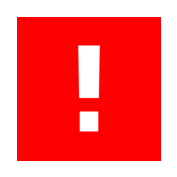
\includegraphics[height=20mm, clip]{figures/info-farbe}
		 	    \hspace{1mm}
					
\includegraphics[height=20mm, clip]{figures/tu-dt-teil-schw-pos}
				\label{fig:TU-Wien}
			\end{figure} 
			
\begin{center}
    \Large
    Research Group Industrial Software (INSO)\\
    Institute for Computer Aided Automation (E183)\\
    Faculty of Informatics\\
    Vienna University of Technology\\

\end{center}

\bigskip

\begin{center}
    \Large
    \centering Master of Science Thesis
    \end{center}
    
\bigskip

\begin{center}
    \Huge\bfseries
    Eine Domain Specific Language zur Berechnung und Evaluierung von Formularfeldern
\end{center}

\bigskip
\bigskip

\begin{center}
    \Large\bfseries
    \noindent
    \centering Autor: \\Thomas Lemm\'{e} \\
    Jahngasse 19, 1050 Wien
\end{center}
\bigskip
\begin{center}
    \Large\bfseries
    \noindent
    \centering Betreuer: \\Thomas Grechenig \\
\end{center}
\bigskip
\begin{center}
    \Large\bfseries
    \noindent
    \centering Wien, \today
\end{center}

\vspace*{\fill}

\cleardoublepage

\rmfamily
\normalfont


\noindent
\emph{Samma felxibl.}
\begin{flushright}
Klaus Feichtinger
\end{flushright}
% *************** Table of contents ***************
\pagenumbering{roman}
\pagestyle{headings}
\renewcommand{\baselinestretch}{0.9}\normalsize
\tableofcontents

% *************** End of front matter ***************

\pagestyle{headings}



\parindent0em
\parskip0.5em

%Zeilenumbrüche vermeiden
\sloppy 

\renewcommand{\baselinestretch}{1.0}\normalsize

\chapter*{Abstract}
Die vorliegende Arbeit beschäftigt sich mit der Modellierung von Ab\-hän\-gig\-kei\-ten in einem medizinischen Studiensystem. 

The fields of a web-form, as well as the underlying data, shall be put in relation using formulas and constraints. When entering data to a field, computations that set the values of dependent fields will be triggered.

The approach used in this master thesis is to design and develop a new expression language called Form Expression Language (FXL). The FXL is a domain-specific language (DSL) in the Domain ``relations in form-based data''. Similar to other expression languages, like formulas in spreadsheed software, FXL-statements are able to use variables to reference other fields and functions to extend the functionality of the language.

The first part discusses the technical and theoretical fundamentals, needed for the understanding of this thesis. An analysis of therms and definition is followed by an overview of the scientific field of relations in webforms. The second part is dedicated to the design process of the language. First the motivation for the development of a new language and its advantages over existing solutions is argued. After that the phases of the software development process, analysis, design, implementation and test, get described. During this process the language and its interfaces have been developed from the requirements.
The third part is about the integration of the FXL in an existing system for medical studies. It describes the system and its workflow to illustrate the use of the FXL in the system. Diverse topics have to be considered: execution time and location, execution order and detection of cyclic dependencies.


\pagenumbering{arabic}

\chapter*{Kurzfassung}
Die vorliegende Arbeit beschäftigt sich mit der Modellierung von Ab\-hän\-gig\-kei\-ten in einem medizinischen Studiensystem. Die Formularfelder eines Web-Formulars sowie die dahinter liegenden Daten, sollen durch Formeln und Bedingungen miteinander in Beziehung gesetzt werden. Durch Eingabe von Werten in einzelne Felder werden Berechnungen ausgelöst, die wiederum den Wert anderer Felder bestimmen.

Der Ansatz, mit dem diesem Problem begegnet wird, ist der Entwurf und die Entwicklung der Ausdruckssprache Form Expression Language (FXL). Diese ist eine Domain Specific Language (DSL) in der Domäne ``Modellierung von Formulardaten''. Ähnlich zu bekannten Ausdruckssprachen, wie etwa den Formel-Ausdrücken aus Tabellenkalkulationssoftware, ist die FXL in der Lage, Statements mit Variablen (zum Referenzieren anderer For\-mu\-lar\-fel\-der) und Funktionen (zur Erweiterung der Funktionalität) zu evaluieren.

Der erste Teil erörtert die zum Verständnis der Arbeit notwendigen technischen und theoretischen Grundlagen. Es werden die Begriffe definiert und eine Über\-sicht über das wissenschaftliche Umfeld der Modellierung von Webformularen geboten.
Der zweite Teil widmet sich dem Entwicklungsprozess der Sprache. Zuerst wird der Aufwand der Entwicklung einer neuen Sprache begründet, indem die Vor- und Nachteile der Alternativen abgewogen werden. Danach werden die Entwicklungsphasen Analyse, Entwurf, Implementierung und Test beschrieben. Im Zuge dieser Phasen wird aus den Anforderungen die Sprache und deren Schnittstellen entwickelt.
Der dritte Teil behandelt die Integration der in dieser Arbeit entwickelten DSL in das medizinische Studiensystem. Nach einer Beschreibung des Zielsystems werden diverse Themen wie Zyklenfreiheit, Ausführungsreihenfolge, Ausführungszeit- und Ort, behandelt, die bei der Integration beachtet werden müssen.



% include chapters here

\chapter{Einleitung}

Die vorliegende Arbeit bewegt sich im Umfeld einer medizinischen Dokumentationssoftware, die zur Eingabe und
Verwaltung von medizinischen Daten verwendet wird. Die Software ist eine Webanwendung, die
Krankenhäusern, Ärzten und anderen Spezialisten den gemeinsamen Zugriff auf Daten für medizinische
Studien ermöglicht. Dabei ist jedoch die Anonymität der Studienteilnehmer gesichert, da medizinische Daten
nur pseudonymisiert und getrennt von Patientendaten abgelegt werden.

Die Software bietet die Möglichkeit, für verschiedene medizinische Fachbereiche bzw. Anforderungen
individuelle Eingabemasken zu erstellen. Dafür können aus unterschiedlichen Formularfeld-Typen flexibel
benutzerdefinierte Formulare erstellt werden. Manche Felder unterliegen dabei Anforderungen, was den Typ
der eingegebenen Daten bzw. den Datenbereich betrifft. In dieser Arbeit soll eine Domain Specific Language (DSL) entwickelt werden, 
welche eine erweiterte Modellierung von Abhängigkeiten und Validierungen in den Eingabemasken ermöglicht.


\section{Motivation}

Die Notwendigkeit für eine generische Lösung zur Berechnung und Eva\-lu\-ie\-rung von Formularelementen
ist begründet durch das Bedürfnis der Benutzer nach Formularen, die automatisch Berechnungen über
mehrere Formulare durchführen. Solche Formulare wurden bisher als eigenes Plugin realisiert, das statt dem Formular 
angezeigt wird. Das Plugin ist somit genau auf den konkreten Anwendungsfall zugeschnitten. Der Nachteil dieser
Lösung ist allerdings, dass für jede Änderung der Sourcecode des Plugins bearbeitet, und die Anwendung 
neu deployed werden muss. Ein weiterer Nachteil ist, dass für jeden weiteren Anwendungsfall mit anderen Berechnungen
ein weiteres Plugin notwendig ist.

Daraus ist die Anforderung nach einer allgemeineren und flexibleren Lösung zur individuellen Modellierung von 
Berechnungen in Formularen entstanden.


\section{Problemstellung}

Um eine flexible Modellierung von Berechnungen in Formularen zu er\-rei\-chen, ist es notwendig, einzelne Felder
automatisch durch arithmetische Operationen mit Werten aus anderen Feldern zu berechnen, wie dies aus diversen
Tabellenkalkulationsprogrammen bekannt ist. Dazu sind zwei verschiedene Arten von Statements notwendig:
Formeln, die einem Feld einen Wert zuweisen und Bedingungen, die den Wert eines Formularfeldes
über\-prü\-fen. Die Eingabe der Statements soll direkt bei der Erstellung eines Formulars in der Webanwendung
geschehen. So ist es beispielsweise zielführend, ein Feld für den Body Mass Index automatisch aus
Körpergröße und Gewicht berechnen zu lassen, anstatt es manuell auszufüllen und bei jeder Änderung der
Daten neu einzugeben.

Ein weiterer wichtiger Teil der Problemstellung ist die Einbettung der Berechnungen und Constraints in das
bestehende Softwaresystem. Da dieses System bereits in Verwendung ist, ist es eine besondere
Herausforderung, die in der Arbeit vorgenommene Implementierung der DSL in das Studiensystem zu integrieren,
ohne die bestehende Architektur oder das Datenmodell im Hinblick auf eine notwendige Migration
maßgeblich zu verändern.


\section{Zielsetzung}

Das Ziel der Diplomarbeit ist, eine Domain Specific Language (DSL) zu ent\-wick\-eln. Dazu ist es notwendig, zu definieren, was eine DSL
ist und was in diesem konkreten Anwendungsfall die Domäne darstellt. Die DSL soll es ermöglichen,
Beziehungen zwischen Formularfeldern herzustellen. Dabei ist darauf zu achten, dass die Syntax einfach
und konsistent ist. Die DSL soll in ihrer Syntax der Schreibweise von bekannten Systemen (Taschenrechner,
Tabellenkalkulation, …) ähnlich sein, so dass diese für erfahrene Computernutzer gut erlernbar und
anwendbar ist.

Der Kern der Arbeit ist der Entwurf und die Entwicklung einer do\-mä\-nen\-spe\-zi\-fi\-schen Sprache und deren
Integration in das bestehende Studiensystem. Der Fokus liegt dabei auf der Funktionalität der
domänenspezifischen Sprache. Nicht Teil der Arbeit sind formularübergreifende Referenzierungen, welche
jedoch in Konzeption und Design berücksichtigt werden. 

Ein Schwerpunkt der Arbeit ist die Integration der DSL in die bestehende Webanwendung. Dabei wird darauf
geachtet, dass die Referenzierung der verschiedenen Formularfelder für Formeln, die Werte aus
mehreren Feldern benötigen, für den Endbenutzer einfach und nachvollziehbar erfolgt. Weiters wird eine
Möglichkeit geschaffen, die Statements der DSL direkt in der Web\-an\-wen\-dung zu den
entsprechenden Formularfeldern einzugeben. Schließlich wird die Ausführung der DSL in die Applikation
integriert, das heißt, wenn Daten eingegeben werden, müssen die angegeben Formeln berechnet, bzw.
Bedingungen überprüft werden. Inwieweit die Ausführung client- oder serverseitig geschieht, wird auch im
Hinblick auf Usability und Antwortzeiten betrachtet.




\section{Struktur}

Die vorliegende Arbeit ist in vier Teile gegliedert.

Der erste Teil, \emph{\nameref{part_grundlagen}}, beschäftigt sich mit der Aufbereitung der für das Verständnis der Arbeit notwendigen fachlichen Themen. Zuerst wird versucht, eine passende Definition des Begriffs `Domain Specific Languages' zu finden (Kapitel \ref{chapter_dsl} \nameref{chapter_dsl}). Kapitel \ref{chapter_theoretische_grundlagen} gibt eine Übersicht über die theoretischen Grundlagen, die zum Verständnis der Arbeit beitragen. In Kapitel \ref{chapter_tools} werden verschiedene Werkzeuge für die Entwicklung vor\-ge\-stel\-lt und insbesondere auf den Parsergenerator ANTLR eingegangen. Ab\-schlie\-ßend wird in Kapitel \ref{related_work} das wissenschaftliche Umfeld aufbereitet.

Im zweiten Teil der Arbeit, \emph{\nameref{part_entwicklung}}, werden die Entwicklungsschritte der aus dieser Arbeit resultierenden DSL beschrieben. Zuerst wird in Kapitel \ref{chapter_entscheidung} die Entscheidung für die Entwicklung einer eigenen Sprache begründet und im Hinblick auf die Alternativen besprochen. Danach werden in der Analyse die Anforderungen an die Sprache erhoben (Kapitel \ref{chapter_analyse}). In Kapitel \ref{chapter_entwurf} wird die DSL beschrieben. Datentypen, semantische Regeln und weitere Features werden genau spezifiziert. Kapitel \ref{chapter_implementierung} beschreibt die Implementierungsdetails der entwickelten Sprache. Kapitel \ref{chapter_test} widmet sich dem Testing in Hinsicht auf die Implementierung.

Der dritte Teil widmet sich der \emph{\nameref{part_integration}}. In Kapitel \ref{chapter_systembeschreibung} wird das medizinische Studiensystem beschrieben, in das die DSL integriert wird. Dazu wird der Workflow erklärt, um dem Leser den Nutzen der DSL im Kontext des Zielsystems zu erläutern. Zusätzlich wird die Architektur sowie der verwendete Technologie-Stack des Zielsystems beschrieben.

Der vierte Teil, \emph{\nameref{part_ergebnis}}, enthält eine Zusammenfassung der Arbeit (Kapitel \ref{chapter_zusammenfassung}). Kapitel \ref{chapter_ausblick} gibt einen Ausblick auf weitere Themen, die über den Umfang dieser Arbeit hinausgehen und Raum für weitere Arbeiten geben.







\part{Grundlagen}
\label{part_grundlagen}
Im folgenden Kapitel werden die Grundlagen von Domain Specific Languages aufgearbeitet. 
Zuerst wird versucht, eine genaue Definition f"ur den Begriff DSL zu finden. 
Anhand von Beispielen wird gezeigt, wie flexibel dieser Begriff verwendet werden kann. 
Danach werden die Grundlagen von formalen Sprachen herausgearbeitet, die f"ur das Verst"andnis der Arbeit von Bedeutung sind. 
Ein weiteres Kapitel widmet sich den verschiedenen Tools, die das Erstellen von Sprachen unterstützen können und geht insbesondere auf das Werkzeug der Wahl, ANTLR, ein.
Das Ende des ersten Teils dieser Arbeit widmet sich dem wissenschaftlichen Umfeld und gibt einen Überblick über weitere Arbeiten und Ansätze.



\newpage

\chapter{Domain Specific Languages}
\label{chapter_dsl}

Dieser Abschnitt beschreibt, was eine DSL ist, vergleicht die Vor-, Nachteile und Unterschiede zu General Purpose Languages (GPL), versucht eine für die vorliegende Arbeit geeignete Definition zu finden und gibt Beispiele für bekannte DSLs.

\section{Definitionen}

Dem Begriff Domain Specific Language steht der der General Purpose Language gegenüber. Mit GPLs lassen sich viele unterschiedliche Problemstellungen lösen, die nicht auf eine Branche oder einen Einsatzbereich beschränkt sind. Bekannte Programmiersprachen, die der Kategorie der GPLs zugerechnet werden, sind beispielsweise Java, C/++/\#, Python etc. GPLs sind also allgemeine Programmiersprachen, die nicht auf eine bestimmte Domäne beschränkt sind. Mit Domäne, oder auch Anwendungsdomäne wird ein abgegrenzter Einsatzbereich bezeichnet, der für diesen charakteristische, bzw. eben domänenspezifische, Anforderungen an ein System stellt.

Eine genaue Definition für den Begriff DSL zu finden, ist nicht einfach, da die Bezeichnung in der wissenschaftlichen Community im Moment sehr inflationär gebraucht wird\footnote{Bevor sich der Begriff DSL etablierte, wurden domänenspezifische Sprachen oft als ``little languages'' bezeichnet\cite{VaDe00}.}. Eine kompakte Definition einer DSL gibt Martin Fowler:

\begin{myquote}
Domain-specific language (noun): a computer programming language of limited expressiveness focused on a particular domain. \cite{Fowl05}
\end{myquote}

Eine sehr ähnliche, aber detailliertere Definition kommt von Mernik et al.:

\begin{myquote}
Domain-specific languages (DSLs) are languages tailored to a specific application domain. They offer substantial gains in expressiveness and ease of use compared with general-purpose programming languages in their domain of application. \cite{MeHe05}
\end{myquote}


Ein Unterschied, der ins Auge sticht, ist, dass Fowler die eingeschränkte Ausdrucksstärke (``limited ex\-pre\-ssive\-ness'') betont, Mernik et al. aber den erheblichen Gewinn an Ausdrucksstärke (``substantial gains in ex\-pre\-ssive\-ness''). Fowler meint damit, dass man durch die Fokussierung auf eine Domain eine Einschränkung des Einsatzbereiches erzwingt. Mernik et al. sehen den Gewinn an Ausdrucksstärke darin, dass mit einem einzelnen Statement in einer DSL mehr ausgesagt werden kann, als mit einem Statement einer GPL, das DSL-Statement ist also ausdrucksstärker.

Die zweite Definition geht im Unterschied zur ersten auf zwei essentielle Eigenschaften ein: Erstens muss eine DSL genau auf eine bestimmte Domain zugeschnitten sein und zweitens muss sie im Gegensatz zu einer GPL im spezifischen Einsatzbereich einfacher anzuwenden sein.

Ein Grund, warum Fowler in seiner Definition auf die Einfachheit im Gegensatz zu einer allgemeinen Programmiersprache verzichtet, mag seine Einteilung in interne und externe DSLs \cite{FoPa10} sein\footnote{Die Klassifikation in interne und externe DSLs ist nicht die einzige. So können sie auch nach Features oder Darstellungsart (textuell, tabellarisch, graphisch etc.) eingeteilt werden\cite{LaJi07}. }:

\subsection{Interne DSL}

Interne DSLs benutzen die Syntax und die Laufzeitumgebung einer GPL. Oft wird unter der Bezeichnung interner (bzw. embedded) DSL eine ent\-spre\-chen\-de API für eine spezifische Domäne verstanden\footnote{Oft wird in diesem Zusammenhang Bjarne Stroustrup, der Entwickler von C++, zitiert: ``Library design is language design''}.
Eine Herausforderung ist das Mapping des domainspezifischen Problems auf eine GPL. Eine sehr beliebte Möglichkeit, APIs eine gewisse ``Sprachähnlichkeit'' zu geben, ist das sogenannte Method Chaining
\cite{RuBa08}.
Bei dieser Technik wird das Objekt, auf dem eine Methode aufgerufen wird, von ebendieser Methode wieder zurückgegeben. So können Methodenaufrufe verkettet werden, was sehr intuitive Statements zur Folge haben kann.

In manchen Sprachen können Sprachfeatures verwendet werden, um die Sprache zu einer eigenen DSL zu erweitern. Die Sprache Java\-Script bietet etwa die Möglichkeit, Typen und Objekte zur Laufzeit dynamisch zu verändern (Listing \ref{listing_javascript_each}).

\begin{lstlisting}[language=JavaScript, caption={Erweiterung des Array-Typs um die Funktion \texttt{each()} in der Java\-Script Bibliothek Prototype},label=listing_javascript_each]
['1', '2', '3'].each(function(elem){
	alert('Number ' +elem);
});
\end{lstlisting}

Eine weitere Möglichkeit, eine interne DSL zu verwenden, bietet die Einbindung einer Laufzeitumgebung einer allgemeinen Programmiersprache in ein Softwaresystem. Eine Methode bietet die Java Plattform mit der Einbettung von verschiedenen Script-Engines (vgl. Abschnitt \ref{section_java_scripting}).

\subsection{Externe DSL} 

Da externe DSLs nicht eingebettet in einer anderen Sprache ausgeführt werden, ist eine eigene Laufzeitumgebung not\-wen\-dig. 

Eine externe DSL ist als individuelle Sprache mit eigener Syntax definiert, die allerdings auch existierende Notationen verwenden kann. Zu\-sätz\-lich zur frei definierten Syntax, muss auch die Semantik explizit definiert werden. Der große Unterschied zu internen DSLs ist, dass die Komplexität der Sprache genau auf die Domäne, für die sie verwendet wird, beschränkt werden kann. Die Erstellung von Interpretern und Übersetzern wird durch eine Vielzahl meist freier Werkzeuge unterstützt.

In der Entscheidungsphase beim Design der DSL zur Berechnung und Eva\-lu\-ier\-ung von Formularfeldern wird nochmals genauer 
auf das Thema interne vs. externe DSLs und deren Vor- und Nachteile im Bezug auf die Aufgabenstellung dieser 
Arbeit eingegangen (Kapitel \ref{chapter_entscheidung}).

Weiters führt Fowler auch noch \textit{Language Workbenches} als eigene Kategorie domänenspezifischer Sprachen auf. 
Darunter versteht man hochintegrierte Entwicklungsumgebungen, die nicht nur die Definition und Generierung von DSLs ermöglichen, 
sondern auch eine Entwicklungsumgebung für die erstellte Sprache zur Verfügung stellen\footnote{Eine der bekanntesten Language Workbenches ist Jetbrains's MPS. Eine Über\-sicht über Language Workbenches und eine 
Vergleichsmatrix findet sich unter http://www.languageworkbenches.net/index.php?title=LWC2011\_Comparison\_Matrix, 20.12.2011}.



\section{Vorteile und Nachteile}

Domänenspezifische Sprachen können einen erheblichen Gewinn an Produktivität und Wartbarkeit mit sich bringen\cite{VaDe98}. DSLs sind für den Endbenutzer besser zu handhaben. Durch die domänenspezifische Notation und der damit einhergehenden besseren Les- und Schreibbarkeit ist es für Domänenexperten leichter, die Sprache zu verwenden. 

Ein weiterer großer Vorteil ist die Validierung und Optimierung der Sprache auf Domain-Level. Das bedeutet, dass dem Benutzer viel detaillierter Feedback über die eingegebenen Programme und eventuell auftretende Fehler gegeben werden kann, als es eine allgemeine Programmiersprache könnte\cite{VaDe00}.

DSLs haben nicht nur Vorteile, sondern auch Nachteile und Einschränkungen. Ein Nachteil ist der not\-wen\-dige Entwicklungsaufwand, um die Sprache zu erstellen. Der Aufwand, der zuerst investiert werden muss, benötigt einen ent\-sprech\-enden Zeitraum, um sich zu amortisieren.

Die domänenspezifische Notation kann sich auch als Nachteil erweisen, weil sie die Möglichkeiten dahingehend einschränkt, dass wirklich nur die dafür vorgesehenen Aufgaben erledigt werden können. Statt einer Erweiterung der Funktion wie in GPLs durch eigene Klassen und Funktionen ist bei einer DSL eine Änderung der Sprachdefinition und der Laufzeitumgebung not\-wen\-dig.

Einen weiteren Nachteil kann der Verlust von Performance und Effizienz einer selbst erstellten DSL im Vergleich zu einer ausgereiften GPL darstellen\cite{VaDe00}.



\section{Beispiele}
\label{grundlagen_examples}

Es finden sich diverse Beispiele für Sprachen, die auf einen eigenen Anwendungsbereich zugeschnitten sind. Nachfolgend werden einige Beispiele vorgestellt, die sich in der Informatik etabliert haben.

\paragraph*{SQL}
(Structured Query Language) ist eine Sprache zur Abfrage und Manipulation von Daten in relationalen Datenbanken. Sie eignet sich sehr gut als Beispiel für eine DSL, da sie die wesentlichen Eigenschaften hat: eine eigene, genau spezifizierte Domäne (Definition, Abfrage, Manipulation von Daten(banken)) und eine eingeschränkte Syntax, die auf die von GPLs bekannten Konstrukte wie Schleifen verzichtet.

\paragraph*{\LaTeX} ist ein Softwarepaket zum Setzen von Texten, das auf der Software \TeX \ aufbaut. Im Gegensatz zu herkömmlichen Textverarbeitungswerkzeugen werden Texte in Latex nicht in einem graphischen Editor bearbeitet, sondern in einem einfachen Textdokument. Elemente wie Überschriften oder Bilder werden im Text mit einfachen Befehlen ausgezeichnet. Das Latex-Dokument kann dann in verschiedene Formate, wie Postscript, PDF oder HTML ausgegeben werden. Wie HTML ist Latex also keine Programmiersprache, sondern eine Auszeichnungssprache.


\paragraph*{EBNF}
(Extended Backus-Naur Form) ist - wie der Name vermuten lässt - eine Erweiterung der Backus-Naur Form. Sie ist eine Metasprache zur Definition von Grammatiken und erlaubt die Darstellung von Produktionsregeln, Nichtterminalsymbolen und Terminalsymbolen in einer leicht verständlichen Form\cite{NiWi77}. Sie definiert Wiederholungen in geschweiften, und optionale Elemente in eckigen Klammern. Alternativen werden durch einen senkrechten Strich getrennt. 

\begin{lstlisting}[float = htbp,caption={Beschreibung eines Fließkomma-Typs in EBNF.},label=listing_example_ebnf]
DECIMAL = {DIGIT} "." DIGIT {DIGIT} | DIGIT {DIGIT} "." {DIGIT};

DIGIT   = "0"|"1"|"2"|"3"|"4"|"5"|"6"|"7"|"8"|"9" ;
\end{lstlisting}

Listing \ref{listing_example_ebnf} Beschreibt einen Fließkomma-Typ DECIMAL mit Hilfe der EBNF. Dieser Typ besteht aus beliebig vielen Ziffern vor und nach dem Kommapunkt, wobei jedoch zu beachten ist, dass mindestens eine Ziffer vor oder nach dem Kommapunkt verpflichtend ist.

Viele Tools zur Generierung von Parsern verwenden eine Abwandlung oder Erweiterung der EBNF zur Beschreibung der Grammatik (vgl. Abschnitt \ref{tools_vergleich}).




\chapter[Theoretische Grundlagen]{Theoretische Grundlagen zum Verständnis der Arbeit}

\label{chapter_theoretische_grundlagen}

In diesem Kapitel werden die theoretischen Grundlagen, die zum Verständnis der Arbeit not\-wen\-dig sind aufbereitet. Diese beinhalten zunächst eine Über\-sicht über die anerkannten Methoden des Übersetzerbaus. Danach folgt eine Ein\-füh\-rung in formale Sprachen, die durch bestimmte Grammatiken erzeugt werden. Das ist vor allem deshalb not\-wen\-dig, um ein Verständnis für die Arbeitsweise von Parsern zu erlangen. Weiters wird auf tiefere Konzepte wie Variablen und Funktionsaufrufe sowie den Umgang mit verschiedenen Datentypen eingegangen.


\section{Language Applications}
\label{theorie_language_applications}

Terence Parr definiert Language Applications nicht nur als Implementierung einer Sprache, sondern ``any program that processes, analyzes, or translates an input file''\cite{Parr10}. Diese allgemeine Definition ist vor allem für DSLs interessant, da diese oft mehr  einer Konfigurationssprache als einer richtigen Programmiersprache ähnlich sind. Für das Auswerten von derart ein\-ge\-schränk\-ten Sprachen ist somit auch nicht unbedingt der volle Umfang eines Parsers, Interpreters oder Übersetzers im klassischen Sinne not\-wen\-dig. Im Kontext dieser Arbeit wird nur ein Teil dieser Definition betrachtet, nämlich die Interpretation (im Sinne von Auswertung) von Ausdrücken, in Hinsicht auf erweiterte Konzepte von allgemeinen Language Applications. Darunter fallen in erster Hinsicht Variablen, Funktionen und Datentypen, die in der DSL verwendet werden sollen.

Der klassische Aufbau einer Language Application, wie er auch in diversen Lehrbüchern und Skripten zum Thema Compilerbau beschrieben ist, besteht aus den  Phasen lexikalische Analyse, syntaktische Analyse, semantische Analyse und Codeerzeugung, wobei im Falle einer interpretierten Sprache an Stelle der Codeerzeugung ein Laufzeitsystem tritt (Abbildung \ref{abb_language_application_klassisch})\footnote{Bei manchen interpretierten Sprachen wird zuerst ein Zwischencode erzeugt, der dann vom Interpreter abgearbeitet wird. Auch der AST (Abbildung \ref{abb_beispiel_ast}) kann als Zwischencode betrachtet werden.}.


\begin{figure}[h]
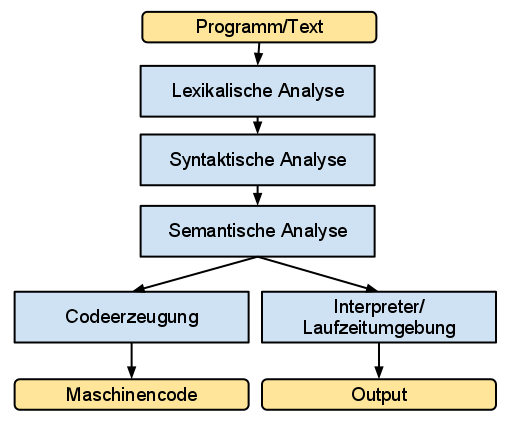
\includegraphics[width=\textwidth,scale=0.5]{figures/language_application_klassisch.png}
\caption{Klassischer Aufbau einer Language Application: Compiler (linker Zweig) und Interpreter (rechter Zweig)}
\label{abb_language_application_klassisch}
\end{figure}

In der lexikalischen Analyse wird das Programm eingelesen und in Tokens\footnote{Oft wird in der deutschsprachigen Literatur das Wort Symbol synonym verwendet.} aufgeteilt. Ein Token ist ein Paar bestehend aus einem Bezeichner oder Typ und einem optionalen Wert\cite[S. 111ff]{AhSe86}. Tokens können Keywords und Operatoren einer Sprache, Bezeichner von Funktionen und Variablen oder Literale sein. Im Zuge der lexikalischen Analyse können auch Zeichen wie Tabulatoren oder Leerzeichen, sofern diese für die Weiterverarbeitung nicht interessant sind, verworfen werden. Die Ausgabe nach dieser Phase ist eine Folge von Tokens, die von der syntaktischen Analyse für das Parsing verwendet wird.

Beim Parsing (syntaktische Analyse) wird versucht, die Tokenfolge den Regeln der zugrundeliegenden Grammatik unterzuordnen. So kann überprüft werden, ob die Eingabe der Syntax der Sprache entspricht. Verschiedene Strategien des Parsens werden in Abschnitt \ref{theorie_parsing_strategien} beschrieben. 

Das Ergebnis der syntaktischen Analyse kann in einem Parse Tree dargestellt werden. Dabei wird zwischen den Formaten Concrete Syntax Tree (CST) und Abstract Syntax Tree (AST) unterschieden (CST in Abbildung \ref{abb_beispiel_cst}, AST in Abbildung \ref{abb_beispiel_ast}). Der CST gibt die der Grammatik der Sprache und deren Ableitungsregeln ent\-sprech\-ende Hierarchie der Tokens, die bei der lexikalischen Analyse identifiziert werden, wieder. Für die Darstellung des AST werden jene Tokens eliminiert, die durch die Struktur des Baumes ihre Bedeutung verlieren\footnote{Im Beispiel in der Abbildung werden etwa die Klammern vor und nach der Addition obsolet, da diese in einem eigenen Subtree dargestellt wird. Zusätzlich werden Ableitungsregeln eliminiert, die nur auf die nächste zeigen und keine semantisch relevanten Verknüpfungen beinhalten}.  

\begin{figure}[h]
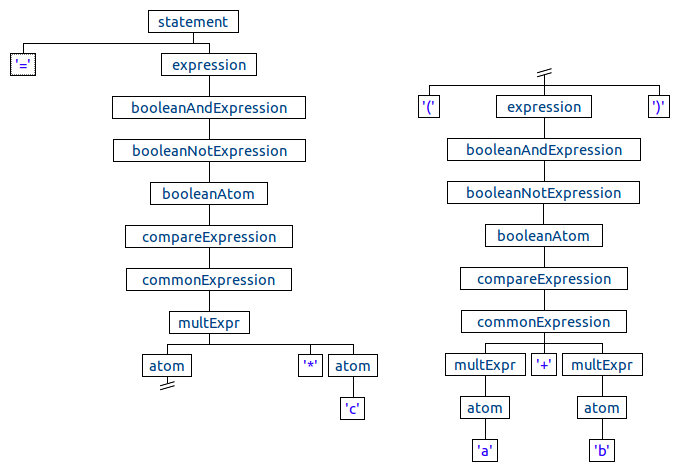
\includegraphics[width=\textwidth,scale=0.2]{figures/cst_beispiel.png}
\caption{Concrete Syntax Tree (CST). Der CST ist ein Baum, der die Ableitungsregeln der Grammatik wiederspiegelt.}
\label{abb_beispiel_cst}
\end{figure}

\begin{figure}[h]
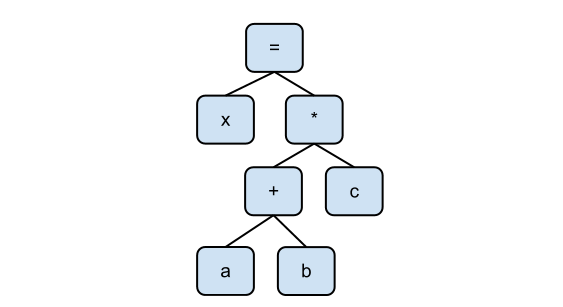
\includegraphics[scale=0.5]{figures/ast_beispiel.png}
\begin{center}
\caption{Abstract Syntax Tree (AST). Der AST ist ein Baum, der die für den Interpreter notwendigen Knoten enthält.}
\end{center}

\label{abb_beispiel_ast}
\end{figure}

Die semantische Analyse überprüft Anforderungen an das Programm, die nicht durch die Syntax abgedeckt werden können. Das betrifft vor allem die Überprüfung, ob ein Programm dem Typsystem entspricht. Das Typsystem setzt sich zusammen aus der Definition der vorhandenen Datentypen und den Regeln zur Zuweisung der Typen zu Operatoren (vgl. \cite[S. 426]{AhSe86}). In vielen Programmiersprachen sind einige Operatoren überladen, d.h. sie können mit verschiedenen Datentypen verwendet werden. In der Phase der semantischen Analyse werden die Rückgabetypen aus dem Kontext abgeleitet. Die Typen von Variablen und Funktionen können aus einer Symboltabelle ausgelesen werden, in welcher Deklarationen derselben gesammelt werden.

Je nach Einsatzzweck wird die Eingabe dann in Maschinencode übersetzt oder in einer Laufzeitumgebung ausgeführt. Beim Compiler ist zu beachten, dass die Codeerzeugungsphase in die Phasen Zwischencodeerzeugung, Codeoptimierung und Codeerzeugung aufgeteilt werden kann. 

Um den Rahmen der Arbeit nicht zu sprengen, möchte ich hier zum tieferen Verständnis der einzelnen Phasen auf das Standardwerk \emph{Compilers: principles, techniques and tools}\cite{AhSe86} verweisen.


\section{Grammatiken}

Um die Syntax einer Sprache festzulegen, ist eine formale Grammatik not\-wen\-dig. Eine formale Grammatik $G \ = (\Sigma,\ N\ ,P\ ,S\ )$ besteht aus einer Menge von Terminalsymbolen $\Sigma$, einer Menge von Nichtterminalsymbolen $N$, den Produktionsregeln $P$, sowie dem Startsymbol $S$\footnote{Eine übersichtliche Ein\-füh\-rung in die verschiedenen Grammatiken, sowie deren Unterschiede, Anwendungen und Normalisierungen, findet man in \cite{VoWi02}.}.

Eine Grammatik beschreibt die Menge aller syntaktisch korrekten Programme einer Sprache. Diverse Sprachen in unterschiedlichen Anwendungen erfordern unterschiedliche Typen von Grammatiken. Eine beliebte Einteilung wurde von Noam Chomsky in der sogenannten Chomsky-Hierarchie vorgenommen:

\begin{myquote}For i = 1, 2, 3, a type i grammar is one meeting restriction i, and a type i language is one with a type i grammar. A type 0 grammar (language) is one that is unrestricted. 
Type 0 grammars are essentially Turing machines; type 3 grammars, finite automata. Type 1 and 2 grammars can be interpreted as systems of phrase structure description. \cite{Chom59}
\end{myquote}

Chomsky definiert also 4 Typen von Grammatiken, die unterschiedlich restriktive Ab\-lei\-tungs\-re\-geln haben:

\begin{itemize}
  \item Typ-0 Grammatiken: Dieser Typ repräsentiert die Menge aller formalen Grammatiken.
  \item Typ-1 Grammatiken: Grammatiken vom Typ 1 werden kontextsensitive Grammatiken genannt.
  \item Typ-2 Grammatiken: Dieser Typ definiert die kontextfreien Grammatiken. Die Syntax der meisten Programmiersprachen kann durch eine kontextfreie Grammatik beschrieben werden.
  \item Typ-3 Grammatiken: Diese sind jene Grammatiken, die durch reguläre Ausdrücke beschrieben werden können.
\end{itemize}

Der für Programmiersprachen relevante Typ ist also die Typ-2 bzw. kontextfreie Grammatik. Diese zeichnen sich dadurch aus, dass auf der linken Seite jeder Produktionsregel genau ein Nichtterminalsymbol steht (also ``frei von Kontext''). Auf der rechten Seite kann jede mögliche Folge von Terminal- bzw. Nichtterminalsymbolen stehen.



Meistens wird die Grammatik einer Sprache in einer Form dargestellt, die der Erweiterten Backus-Naur Form (EBNF, siehe Abschnitt \ref{grundlagen_examples}) ähnlich ist. In dieser Form sind die verschiedenen Bestandteile der Grammatik der Sprache (Terminal- bzw. Nichtterminalsymbole, Startsymbol und Produktionsregeln) gut ersichtlich und einfach nachzuvollziehen.

Je nach Parsingalgorithmus unterliegen die Grammatiken bestimmten Regeln, um vom Parser verarbeitet werden zu können.


\section{Parsing Strategien}
\label{theorie_parsing_strategien}

Ein Parser ist, allgemein gesprochen, ein Programm oder eine Softwarekomponente, die eine Eingabe in ein weiter verarbeitbares Format umwandelt. Es gibt verschiedene Ansätze, wie diese Aufgabe erfüllt werden kann. Grund\-sätz\-lich ist es möglich, eine Eingabe Top-Down oder Bottom-Up zu verarbeiten.

\subsection{Top-Down Analyse}

Bei der Top-Down Analyse wird versucht, ausgehend vom Startsymbol Ab\-lei\-tun\-gen zu finden, mit denen das gegebene Wort eingelesen werden kann. Dazu muss eine Tabelle erstellt werden, die jedem Eingabesymbol die ent\-sprech\-en\-de Produktionsregel zuordnet. Die Eingabe wird dann von links nach rechts mittels Linksableitungen abgearbeitet. Die Menge der Grammatiken, die mit dieser Methode verarbeitet werden können, werden LL(k) Grammatiken genannt. Das \emph{k} steht für den Lookahead, der notwedig ist, wenn einem Eingabesymbol mehrere Regeln in der Tabelle zugeordnet werden.


\subsection{Bottom-Up Analyse}

Die Bottom-Up Analyse geht den umgekehrten Weg, von der Tokenfolge zum Startsymbol. Sie versucht, in einer Eingabe eine Struktur zu finden, die den syntaktischen Regeln der Sprache entspricht. Nach und nach werden, abhängig vom Lookahead, ein oder mehrere Symbole eingelesen und davon ausgehend eine Produktionsregel aufgelöst.


\subsection{Erweiterte Konzepte und Optimierungen}
\label{theorie_erweiterte_konzepte}

\subsubsection{Backtracking} 

Unter Backtracking versteht man das Ausprobieren verschiedener Alternativen bei mehrdeutigen Produktionsregeln. Wenn eine Ableitung fehlschlägt, wird die Eingabe bis zur letzten Kreuzung zurückgespult und die nächste Alternative versucht. Erst wenn alle Alternativen erschöpft sind, wird ein Fehler zurückgegeben. Backtracking kann sehr aufwendig sein, da einzelne Regeln für eine Eingabe öfters aufgerufen werden. Um diese Mehrfachaufrufe zu reduzieren, kann eine Technik namens Memoization eingesetzt werden.

Zu beachten ist, dass unter Umständen Actions im Parser wiederholt oder umsonst ausgeführt werden, da Regeln aufgerufen werden, die im Endeffekt gar nicht benötigt werden.

\subsubsection{Memoization}

Memoization ist eine allgemeine Optimierungstechnik, um zu vermeiden, dass Funktionen, die das gleiche Resultat zurückgeben,  wiederholt aufgerufen werden. Im Kontext des Parsing bedeutet dies, dass das Resultat von Ab\-lei\-tungs\-re\-geln zwischengespeichert wird. Wenn eine Regel aufgerufen wird, kann zuerst in der Tabelle nachgesehen werden, ob bereits ein Resultat vorliegt. Wenn dies der Fall ist, muss die Regel nicht noch einmal ausgeführt werden.

Memoization erfordert zwar einen höheren Speicheraufwand beim Parsen, beschleunigt aber das Verfahren, da der Lookup wesentlich effizienter ist, als das wiederholte Parsen von Teilausdrücken.

\section{Typisierung}

Die meisten Programmiersprachen definieren verschiedene Datentypen, bzw. erlauben die Definition eigener Typen. Die Typisierung kann dabei statisch oder dynamisch erfolgen. Statische Typsysteme haben den Vorteil, dass sie bereits bei der Übersetzung überprüft werden können. Sie erhöhen somit die Wahrscheinlichkeit, dass das eingegebene Programm korrekt ist. Auch die Effizienz kann gesteigert werden, da eine Überprüfung zur Laufzeit nicht mehr not\-wen\-dig ist. Bei dynamischen Typsystemen erfolgt die Zuweisung von Typen zu Variablen und Funktionen, und somit auch deren Überprüfung, erst zur Laufzeit des Programmes.

Da die Syntax einer Sprache im Großen und Ganzen unabhängig von der Typisierung ist, ist vor allem die semantische Analyse für die Typ\-über\-prü\-fung zuständig. Lässt die Sprache die Deklaration von Variablen und Funktionen zu, muss deren (Rückgabe-) Typ in einer Symboltabelle abgespeichert werden. Wird die Variable oder Funktion in einem Statement des Programmes verwendet, muss der ent\-sprech\-ende Typ aus der Symboltabelle abgerufen werden.

Ein Teil des Typsystemes ist die Zuordnung von Typen zu Operatoren. Da die meisten Operatoren überladen sind, müssen die tatsächlichen Typen während der Typ\-über\-prü\-fung aus dem Kontext abgeleitet werden. Bei Funktionsaufrufen ist zusätzlich eine implizite Typumwandlung not\-wen\-dig. Das bedeutet, dass ein Typ in einen anderen umgewandelt werden kann, wenn dies keine semantische Än\-der\-ung\-en zur Folge hat. Ein Beispiel ist eine Funktion mit einem Parameter vom Typ Gleitkommazahl. Ohne den Sinn der Funktion zu verändern, kann auch eine Ganzzahl an die Funktion übergeben werden, da die Menge der Ganzzahlen -- mathematisch gesehen -- eine Teilmenge der Gleitkommazahlen ist.


\chapter{Werkzeugunterstützung}
\label{chapter_tools}

Natürlich wäre es auch möglich, den Parser zur Verarbeitung der DSL-Statements ''per Hand'' zu programmieren. Allerdings bietet sich die Verwendung von vorhandenen Werkzeugen natürlich an. Die Verwendung von Tools hat neben dem einfacheren Entwicklungsprozess auch positive Aus\-wir\-kun\-gen auf die Wartbarkeit der DSL:

\begin{myquote}
Our results suggest that DSL tools do indeed increase maintainability
of DSL implementations. Especially our code reduction measurements
corroborate the hypothesis. The use of a DSL tool does
not necessarily make the resulting implementation less complex in
a structural sense, but it does usually remove the need for boilerplate
structure. \cite{KlSt10}
\end{myquote}

Es existieren viele verschiedene Werkzeuge und Frameworks im  Java-Umfeld, die die Entwicklung von DSLs unterstützen. Diese unterscheiden sich al\-ler\-dings stark in den gebotenen Möglichkeiten, aber auch in den Methoden, was sicherlich auch an der unscharfen Definition des Begriffs DSL liegt. Manche Tools bieten eine gute Integration in eine Entwicklungsumgebung (Integrated Development Environment, IDE) oder eine eigene Entwicklungsumgebung, einige generieren sogar Editoren, um die entwickelte DSL anzuwenden, andere sind simple Kommandozeilenprogramme.

Für die in dieser Arbeit zu entwickelnde DSL sind vor allem Parsergeneratoren, auch Compiler-Compiler genannt, interessant. Diese Tools generieren aus einer Grammatik in einem bestimmten, je nach Tool unterschiedlichen, Format einen Lexer und einen Parser (oder eine Kombination aus beiden). Der Output des Parsers, zumeist ein AST, kann in weiterer Folge verwendet werden, um einen Interpreter oder Übersetzer zu erstellen.


\section{Über\-sicht}

Bei allen Tools, die in diesem Abschnitt erwähnt werden, handelt es sich um Parsergeneratoren. Allen gemeinsam ist, dass sie die Grammatik einer Sprache in einem anwendungsabhängigen Format einlesen und verarbeiten. Das Produkt eines Parsergenerators ist ein lauffähiger  Parser (bzw. zusätzlich ein Scanner\footnote{Bei manchen Tools ist der Scanner im Parser integriert. Allerdings kann ein Scanner als eigene Komponente verwendet werden, um Informationen über ein Programm auszulesen, für die nur die Tokens benötigt werden. Der Scanner wird bei der FXL z.B. verwendet, um alle Variablen einer Formel zu erhalten, indem die Tokens vom Typ VAR aus der Tokenfolge ausgelesen werden. Siehe auch Abschnitt \ref{theorie_language_applications} bzw. der Algorithmus zur Bestimmung der Aus\-führ\-ungsreihenfolge in Abschnitt \ref{implementierung_integration_reihenfolge}.}), der ein Programm in der zu entwickelnden Sprache in einen AST verwandelt (Abbildung \ref{abb_parser_generator_workflow}). 

Eine weitere Möglichkeit ist, Ausdrücke bereits beim Parsen auszuwerten. Die meisten Tools unterstützen Actions, die bei der Aus\-führ\-ung einer Ab\-lei\-tungs\-re\-gel im Parser ausgeführt werden. Diese Möglickeit hat allerdings einige Nachteile:

\begin{itemize}
  \item Die Actions werden direkt in die Grammatikdatei geschrieben und machen so die eigentliche Grammatik schlecht lesbar.
  \item Die Statements der Actions werden in der Zielsprache des Parsers eingegeben. Editoren für Grammatiken unterstützen allerdings nicht den Umfang eines Codeeditors einer IDE, was die Entwicklung fehleranfälliger und schwieriger macht.
  \item Verwendet der Parser Backtracking, kann es sein, dass einige Actions mehrfach ausgeführt werden.
  \item Typechecks ohne Aus\-führ\-ung des Statements wären nur durch eine eigene Grammatik für diesen Zweck möglich, was zu Redundanz und erhöhter Fehleranfälligkeit führt.
\end{itemize}

Für diese Arbeit wurde entschieden, dem Prinzip der \emph{Separation of Concerns} zu folgen und den erzeugten AST in einem Typechecker bzw. Interpreter explizit abzuarbeiten.

 

\begin{figure}[h]
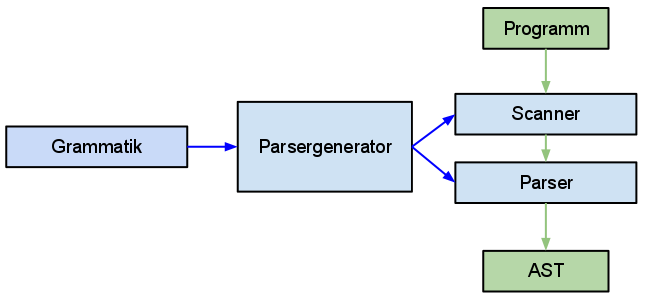
\includegraphics[scale=0.6]{figures/parser_generator_workflow}
\caption{Workflow eines Parser Generators (blau).}
\label{abb_parser_generator_workflow}
\end{figure}



\section{Vergleich}
\label{tools_vergleich}

Um eine Auswahl für die Implementierung des Interpreters zu treffen, ist es not\-wen\-dig, die verschiedenen Tools anhand verschiedener Eigenschaften zu vergleichen. Das betrifft vor allem das Format der Grammatik und die vorhandenen Ein-/Ausgabesprachen.
Zu\-sätz\-liche Faktoren sind die Werkzeugunterstützung (Grammatikeditor, Rule-Visualisierung, (Concrete/Abstract) Syntax Tree-Visualisierung), Dokumentation und (Community-) Support sowie Tools für den Build-Prozess.

In diesem Kapitel werden die Tools ANTLR, Coco/R und JavaCC verglichen. Diese sind alle für die Java-Plattform verfügbar und grund\-sätz\-lich für die in dieser Arbeit zu entwickelnde Sprache geeignet. Zu\-sätz\-lich können diese Produkte als ausgereift betrachtet werden und wurden erfolgreich in verschiedenen Projekten eingesetzt.


\subsection{ANTLR}

Der Parsergenerator ANTLR wird von Terence Parr seit 1989 an der Universität von San Francisco entwickelt und hat sich zu einem Quasi-Standard auf der Java Enterprise Plattform entwickelt. Unter anderem wird ANTLR im Applicationserver Weblogic, dem ORM-Mapper Hibernate, der IDE IntelliJ IDEA oder der JBoss Rules Engine Drools eingesetzt\footnote{vgl. http://www.antlr.org/showcase/list, 23.3.2012}.

ANTLR ist in Java implementiert, unterstützt aber diverse Zielsprachen wie Java, C++, C\#, Ruby, Objective C uvm. Für die Entwicklung steht eine ausgeprägte Palette an Tools zur Verfügung (siehe Abschnitt \ref{tools_antlr_tools}). Die Grammatik ist ein Format, das sich an der EBNF-Notation orientiert, aber erweiterte Konzepte wie Actions und Attribute zum Aufbau eines AST unterstützt. Lexikalische und syntaktische Regeln können in separaten Files abgelegt werden.

Neben der ausführlichen Dokumentation auf der Projektwebseite existiert auch ein Buch des Autors als Einführung und Referenz\cite{Parr07}. Aufgrund der weiten Verbreitung in der Java-Welt steht ausreichend Support durch die Community zur Verfügung.



\subsection{Coco/R} 

Das Coco/R Projekt\cite{HaMo90} ist ein Parsergenerator, der ursprünglich von Hans\-peter Mössenböck an der Universität Linz entwickelt wurde. Zwischenzeitlich wurde das Projekt an der ETH Zürich fortgesetzt und ist inzwischen wieder an der Universität Linz beheimatet.

Coco/R ist nicht auf eine Plattform beschränkt und unterstützt diverse Spra\-chen. Es existieren Portierungen für u.A. Java, C++, C\# und VB.NET. Als Basis für die Angabe der Grammatik wird die EBNF-Notation verwendet. Angereichert wird diese durch Attribute und \emph{semantic Actions}. Durch diese Attribute kann ein AST aufgebaut werden\footnote{vgl. \cite{Moes11}}, allerdings muss dazu, im Gegensatz zu ANTLR, die ganze Grammatik abgeändert werden.

Auf der Homepage des Projekts steht ein ausführliches User Manual, sowie ausreichend Beispiele für jede Sprach-Portierung zum Download bereit. Zu\-sätz\-lich bietet eine Mailingliste der Universität Linz Support. Es existiert ein Eclipse-Plugin für einen Grammatikeditor und die Erzeugung des Parsers beim Build.

\subsection{JavaCC}


JavaCC ist ein aus dem Sun-Projekt Jack entstandener Parsergenerator für die Java-Plattform. Auf der Projekthomepage wird er als ``the most popular parser generator for use with Java [tm] applications''\footnote{vgl. http://javacc.java.net/, 29.11.2011} bezeichnet. Eine Untermauerung für diese Behauptung, z.B. durch Projekte die JavaCC einsetzen, ist nicht zu finden. Laut Wikipedia\footnote{vgl. http://de.wikipedia.org/wiki/JavaCC, 29.11.2011} verwenden die Suchmaschine Lucene und das Ontologie-Framework Cyc durch JavaCC erstellte Parser.

Die Syntax wird in einer Grammatikdatei definiert, in der sowohl lexikalische als auch syntaktische Regeln angegeben werden. Die Ab\-lei\-tungs\-re\-geln enthalten zwei Blöcke: einen für die Ab\-lei\-tungs\-re\-gel und einen für die Auswertung (sogenannte \emph{Action}) der Regel. Alternativ kann mithilfe des Tools JJTree ein Syntax-Baum erstellt werden.

Die Dokumentation ist recht ausführlich gestaltet. Für Support durch die Community steht eine Mailingliste zur Verfügung. Es gibt ein Eclipse-Plugin, das einen Code-Editor für JavaCC Grammatiken enthält. JavaCC ist in Java geschrieben und generiert Parser ausschließlich in Java.





\section{ANTLR}
\label{tools_antlr}
Dieser Abschnitt setzt sich im Detail mit ANTLR, dem Werkzeug der Wahl für diese Arbeit, auseinander. Wie bereits in Abschnitt \ref{tools_vergleich} erwähnt, sind alle angeführten Tools grund\-sätz\-lich für die DSL geeignet. Die endgültige Entscheidung für die Entwicklung die Form Expression Language (FXL) ANTLR einzusetzen, begründet sich durch die hervorragende Dokumentation, insbesondere dem Buch des Autors, dem guten IDE Support und der Integration in das Build-Tool Maven.


\subsection{Grammatik}

Wie in Abschnitt \ref{tools_vergleich} erwähnt, orientiert sich das Format der Metasprache des Parsergenerators an der EBNF. Zu\-sätz\-lich werden weitere Angaben und Optionen in der Grammatikdatei gespeichert. Als Beispiel einer kompletten Grammatik kann jene der FXL im Anhang betrachtet werden.

\subsubsection{Optionen und zusätzliche Angaben}

Es ist möglich, die Erzeugung von Parser und Lexer durch diverse Einstellungen zu beeinflussen.

\paragraph{Options}

Am Anfang eines Grammarfiles steht eine Auflistung von Parametern in einem \texttt{options}-Block. Diese steuern grundlegende Eigenschaften des generierten Parsers:

\begin{itemize}
  \item Ausgabesprache: Wie in Abschnitt \ref{tools_vergleich} erwähnt, beherrscht ANTLR diverse Ausgabesprachen. Hier muss angegeben werden, in welcher Sprache Lexer und Parser generiert werden sollen.

  \item Ausgabeformat: Das Format, das vom Parser beim Parsen eines Eingabestrings zurückgegeben wird. Dies kann entweder ein AST oder ein StringTemplate\footnote{StringTemplate ist eine Template Engine für verschiedene Einsatzbereiche. http://www.stringtemplate.org/, 23.3.2012} Template sein. Wird die Option weggelassen, wird nichts generiert, der Parser arbeitet dann als Recognizer, der nur den Eingabestring verarbeitet und im Fehlerfall eine Fehlermeldung ausgibt.

  \item Weitere Optionen: Weitere Optionen umfassen vor allem optimierende Parsingstrategien wie Memoizing und Backtracking (siehe Abschnitt \ref{theorie_erweiterte_konzepte}). Eine genaue Auflistung der Optionen befindet sich in der Re\-fe\-renz\cite{Parr07}.
\end{itemize}



\paragraph{Tokens umbenennen}

Literale können einfach als Strings, eingeschlossen in einfachen Anführungszeichen, in der Grammatik verwendet werden (siehe Listing \ref{listing_grammar_tree_compare}). Um diese Literal-Tokens im Interpreter besser verwenden zu können, bietet es sich an, diese mit sprechenden Namen zu benennen. Durch die Angabe \texttt{OR = 'OR';} im \texttt{tokens}-Block, wird im Parser automatisch eine Konstante \texttt{Parser.OR} generiert, auf die beim Abarbeiten des AST zugegriffen werden kann.

Weiters können auch Tokens erstellt werden, die in den Ab\-lei\-tungs\-re\-geln gar nicht vorkommen, aber für den Aufbau des AST benötigt werden. Ein Beispiel ist der \texttt{CALL}-Token in Listing \ref{listing_grammar_tree_function}, der beim Rewrite des AST verwendet wird (siehe folgender Abschnitt).

\subsubsection{Modellierung des Abstract Syntax Trees}

Würde man zur Weiterverarbeitung nach dem Parsen den Concrete Syntax Tree (CST) verwenden, würden die zahlreichen Knoten einen erheblichen Mehraufwand bedeuten. Deshalb ist es wichtig, wie der AST, der dann im Interpreter verwendet wird, aufgebaut sein soll. Dazu bietet ANTLR die Möglichkeit, in der Grammatik zu spezifizieren, wie der Baum aussehen soll. Das kann auf zwei Arten geschehen: inline oder explizit als Rewrite-Regel.

Bei der Inline-Angabe (Listing \ref{listing_grammar_tree_compare}) wird nur jenes Element (Literal, Terminal, oder Nonterminalsymbol) ausgewählt, welches als Wurzelelement des AST-Knotens gewählt wird. Die übrigen Elemente werden in der Reihenfolge ihres Auftretens als Kindelemente an\-ge\-hängt. Elemente, die im AST ignoriert werden sollen, weil sie in der Baumdarstellung ihre Relevanz verlieren (z.B. Klammern, Trennzeichen etc.), werden mit einem Rufzeichen markiert und nicht als Kindelement zum Knoten hinzugefügt.


\begin{lstlisting}[float = htbp,caption={Inline-Regeln zur Beschreibung der Baumstruktur.},label=listing_grammar_tree_compare]
compareExpression
  	:
  	commonExpr (('<'|'>'|'='|'<='|'>='|'!=')^ commonExpr)?
  	;

\end{lstlisting}

Rewrite Regeln können die Baumstruktur auch stark verändern und Knoten einführen, die als solches nicht in der Regel vorkommen. Dazu wird die Regel wie in Listing \ref{listing_grammar_tree_function} einfach an die rechte Seite der Ab\-lei\-tungs\-re\-gel an\-ge\-hängt. Nun kann der Knoten für diese Regel im Format \texttt{\textasciicircum(Root Child1 ... Childn)} angegeben werden, wobei Root den Tokentyp des AST-Knotens bezeichnet, gefolgt von den Kindknoten. 


\begin{lstlisting}[float = htbp,caption={Rewrite-Regeln zur Beschreibung der Baumstruktur.},label=listing_grammar_tree_function]
functionCall
  :
  ID '(' arguments ')' -> ^(CALL ID arguments?)
  ;
\end{lstlisting}

Im Beispiel in Listing \ref{listing_grammar_tree_function} wird der Tokentyp \texttt{CALL} als Typ des Knotens festgelegt. Dazu muss dieser Token allerdings zuerst im Token-Abschnitt des Grammarfiles festgelegt werden (siehe oben). Als erstes Kindelement wird ein Knoten vom Typ \texttt{ID} erstellt, der den Namen der Funktion enthält. Die weiteren Kindknoten sind die optionalen Argumente, wobei diese wiederum komplexe Ausdrücke in Form von Subtrees enthalten können (siehe FXL-Grammatik im Anhang).

\begin{figure}[h]
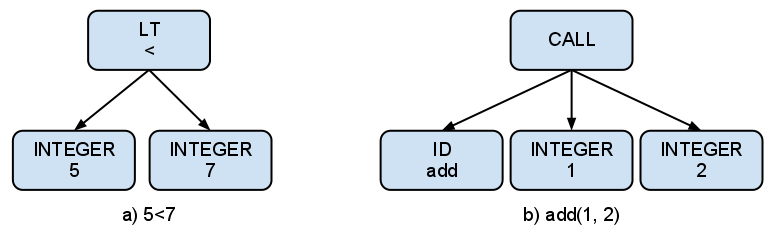
\includegraphics[scale=0.5]{figures/ast_beispiele}
\caption{a) Aufbau des AST bei Inline-Notation. b) Aufbau des AST bei Rewrite-Notation}
\label{abb_ast_beispiele}
\end{figure}

Abbildung \ref{abb_ast_beispiele} Zeigt jeweils ein Beispiel für die zwei Tree-Building Methoden. Die Knoten enthalten jeweils den Tokentyp und den Text des Knotens. In Beispiel a) wird das Kleiner-Zeichen als Wurzelelement verwendet, die anderen Elemente werden als Knoten vom Typ Integer als Kindknoten an\-ge\-hängt. Beispiel b) zeigt den Sonderfall des künstlichen Tokens \texttt{CALL} aus Listing \ref{listing_grammar_tree_function}, der nur zum Umformen des Baumes verwendet wird.


\subsection{Tools}
\label{tools_antlr_tools}

Werkzeuge können den gesamten Entwicklungsprozess effizienter und einfacher gestalten. Sei es durch Tools wie einem Editor oder Debugger bei der Programmierung, oder solche zur Automatisierung des Buildprozesses. Vor allem Integrierte Entwicklungsumgebungen (IDEs) unterstützen den Entwickler beim Design einer Sprache. Im Falle eines Parsergenerators besteht eine IDE aus einem guten Editor für die Grammatik (Syntax Highlighting, Code Completion etc.), visuellen Darstellungen der Grammatik und einzelner Regeln, sowie einer Testumgebung zur Eva\-lu\-ier\-ung der Syntax.

\subsubsection{ANTLRWorks}

ANTLRWorks\footnote{vgl. http://www.antlr.org/works/index.html, 23.3.2012} ist ein Tool zum Entwickeln von Grammatiken für ANTLR. Es ist in vielerlei Hinsicht eine Hilfestellung, da es vor allem visuelle Hilfestellungen, wie Syntaxdiagramme oder Syntaxbäume, bietet. Der Hauptteil von ANTLRWorks besteht aus dem Grammatikeditor und der Auflistung der Grammatikregeln. Der Editor selbst bietet einige Features, die von anderen IDEs bekannt sind wie etwa Syntax Highlighting und Code Completion.

\begin{figure}[h]
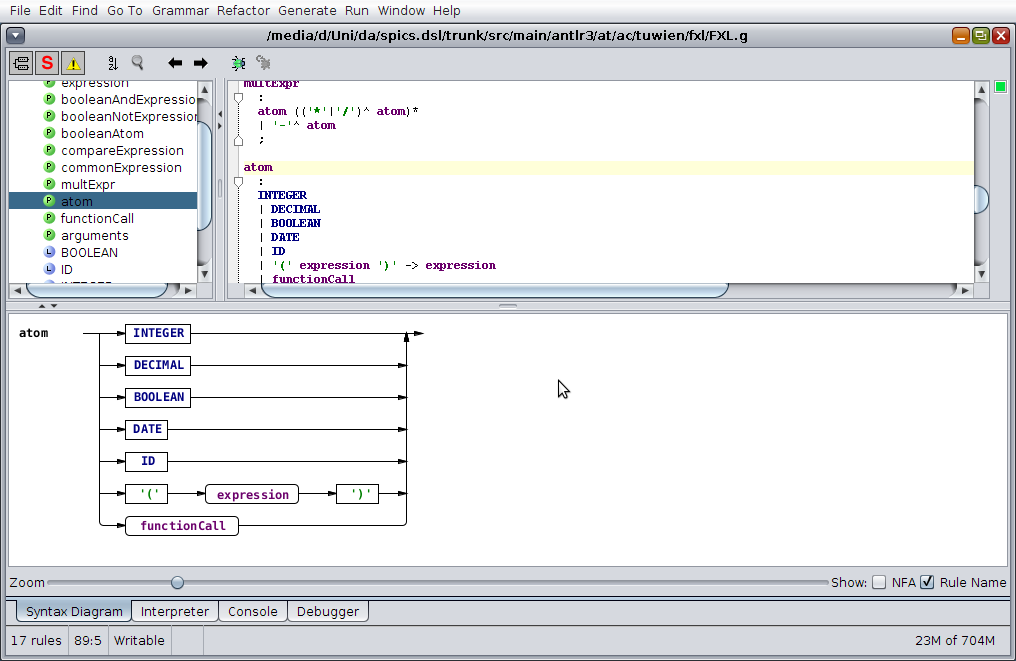
\includegraphics[scale=0.35]{figures/antlrworks_syntax_diagram}
\caption{Syntax Diagram in ANTLRWorks}
\label{abb_antlrworks_syntax_diagram}
\end{figure}

Ein weiteres Feature ist die Darstellung der Regeln in Syntaxdiagrammen (Abbildung \ref{abb_antlrworks_syntax_diagram}). Syntaxdiagramme werden dazu verwendet, Grammatiken graphisch darzustellen. Insbesondere können einzelne Regeln, die textuell durch Verzweigungen und Wiederholungen recht schnell komplex werden, mit Hilfe von Syntaxdiagrammen recht einfach nachvollzogen werden.

\begin{figure}[h]
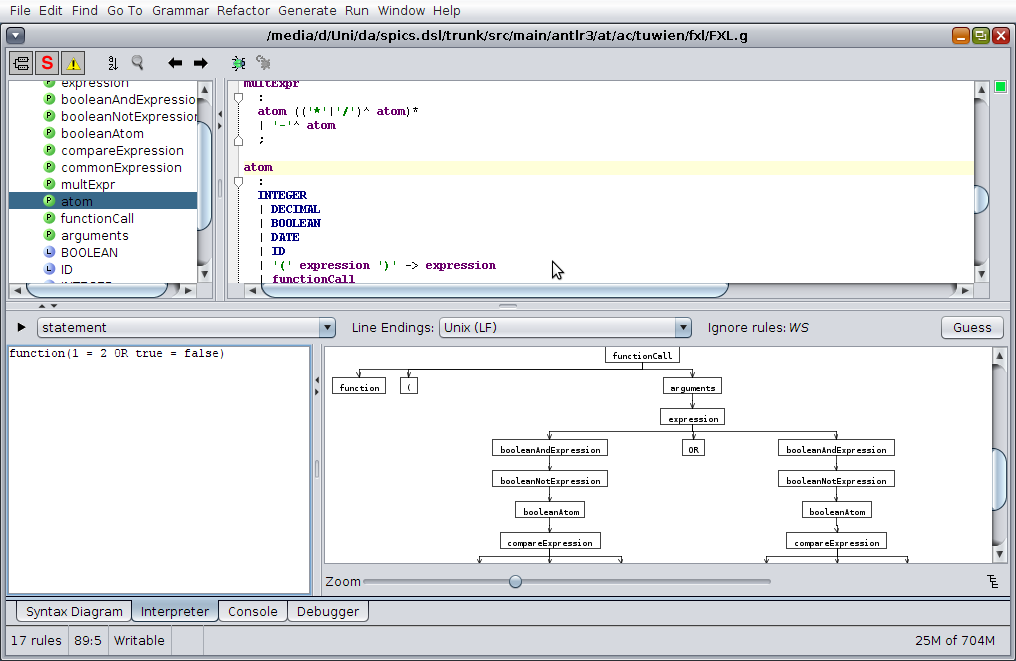
\includegraphics[scale=0.35]{figures/antlrworks_interpreter}
\caption{Interpreter/Concrete Syntax Tree in ANTLRWorks}
\label{abb_antlrworks_interpreter}
\end{figure}

ANTLRWorks kann auch beliebige Eingabestrings parsen und gegen die verschiedenen Ab\-lei\-tungs\-re\-geln testen. Der resultierende Parsebaum wird graphisch dargestellt (Abbildung \ref{abb_antlrworks_interpreter}). Tritt ein Fehler auf, so wird das Parsen unterbrochen und die Stelle im Parsebaum, an der der Parser nicht fortsetzen kann, markiert. Auf diese Art können nicht nur Statements, die von der Startregel ausgehen, getestet werden, sondern auch Eingaben für beliebige Unterregeln.


\begin{figure}[h]
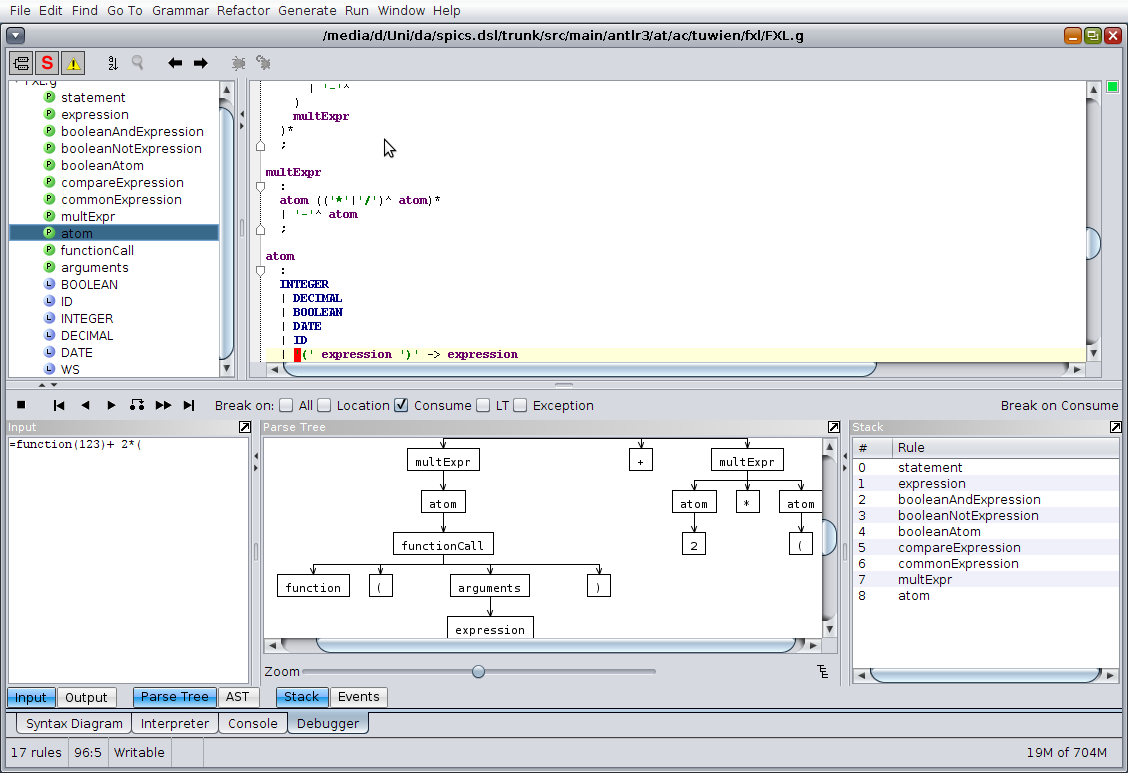
\includegraphics[scale=0.35]{figures/antlrworks_debugger}
\caption{Der Debugger von ANTLRWorks}
\label{abb_antlrworks_debugger}
\end{figure}

Ein Key-Feature von ANTLRWorks ist der Debugger (Abbildung \ref{abb_antlrworks_debugger}). Mit Hilfe des Debuggers lässt sich der Parseprozess Schritt für Schritt nachvollziehen. Während des Parsens wird für jeden Schritt angezeigt, welche Regel gerade angewendet wird. Zu\-sätz\-lich wird der Parsebaum im mittleren Fenster schrittweise aufgebaut.

ANTLRWorks beherrscht sogar das Debuggen von Parsern in anderen Spra\-chen. Dies ist möglich, da ANTLRWorks per Sockets mit dem Parser kommuniziert\footnote{ vgl. http://www.antlr.org/works/index.html, 23.3.2012}.


ANTLRWorks ist ein mächtiges Werkzeug, das den Entwickler effektiv bei der Entwicklung von Grammatiken unterstützt. Der Nachteil ist jedoch, dass es ein eigenständiges Tool ist, dass zusätzlich zu diversen anderen Tools in den Entwicklungsprozess eingebunden werden muss. Für eine bessere Integration in diesen stehen diverse IDE-Plugins zur Verfügung, die im folgenden Abschnitt behandelt werden.
 
\subsubsection{IDE-Plugins}

Mittlerweile existieren diverse Plugins für die wichtigsten Entwicklungsumgebungen\footnote{Eine aktuelle Über\-sicht über die Plugins für diverse IDEs findet sich unter http://www.antlr.org/wiki/display/ANTLR3/Integration+with+Development+Environments}. Für IntelliJ IDEA existiert ein Plugin, das ANTLRWorks direkt in die IDE integriert. Der Funktionsumfang ist dement\-sprech\-end gleich umfangreich wie ANTLRWorks selbst.

Für die weit verbreitete offene IDE Eclipse existieren zwei Plugins. AntlrDT stellt vor allem einen Code-Editor und die Integration in den Eclipse Buildprozess (automatisches Compilieren nach Clean bzw. Speichern) zur Verfügung. Zu\-sätz\-lich bietet das Plugin auch die Visualisierung von ASTs an, die allerdings, im Vergleich zu ANTLRWorks, nicht so ausgereift erscheint. Das zweite Eclipse-Plugin ist ANTLR IDE\footnote{http://antlrv3ide.sourceforge.net/, 23.3.2012}. Es ist sehr ausgereift und wurde auch für die Implementierung der Form Expression Language in der vorliegenden Arbeit verwendet. Es bietet einen Grammatikeditor, eine Ansicht für Syntaxbäume (im Plugin Railroad View genannt) und einen Interpreter, mit dem wie in ANTLRWorks Eingaben auf verschiedene Regeln angewendet werden können. Auch ein Debugger ist vorhanden, der allerdings im Gegensatz zu ANTLRWorks nur mit Java-Parsern arbeiten kann.

\subsubsection{Build Tools} 

Alle oben genannten Plugins integrieren ANTLR in den Buildprozess der Entwicklungsumgebung. Für ANTLR bedeutet dies, dass Lexer und Parser automatisch beim Build der Software aus der Grammatik generiert werden. Oft wird allerdings ein externes Tool zum Build bzw. zur Auslieferung von Software verwendet. Für die zwei verbreitetsten Buildtools auf der Java-Plattform, Apache Ant und Apache Maven, existieren Erweiterungen, die die Codegenerierung übernehmen\footnote{vgl. http://www.antlr.org/wiki/display/ANTLR3/How+to+use+ant+with+ANTLR3 bzw. http://www.antlr.org/antlr3-maven-plugin/index.html}.



\chapter{Related Work}
\label{related_work}

In diesem Kapitel wird eine Über\-sicht über das wissenschaftliche Umfeld dieser Arbeit geboten. Einige der vorgestellten Ansätze und Projekte gaben Anregungen für die Form Expression Language, die in dieser Arbeit entwickelt wurde. Es lassen sich zwei Bereiche identifizieren, die dem Umfeld der Arbeit entsprechen. Einerseits verschiedene Sprachen zur Berechnung und Eva\-lu\-ier\-ung von Werten, andererseits DSLs zur Modellierung von Webformularen. Die Themen Domain Specific Languages und Parser Generatoren wurden bereits weiter oben behandelt.

\section{Sprachen zur Berechnung und Eva\-lu\-ier\-ung von Werten}

Eine Sprache, die sich in wissenschaftlichen Arbeiten oft wiederfindet, ist die Object Constraint Language (OCL)\cite{RiGo98}.Die Object Constraint Language (OCL) ist ein Teil der UML - Spezifikation und wurde ursprünglich für die Modellierung von Klassen- und Sequenzdiagrammen angedacht. Ein weiterer Einsatzort ist die Modellgetriebene Entwicklung. Dort wird OCL etwa im Bereich Transformation von (Meta-) Modellen und Modelchecking verwendet\footnote{vgl. http://www.eclipse.org/modeling/mdt/?project=ocl, 21.3.2012}. Escott et al.\cite{Esco12} setzen die OCL zur Validierung von Webformlaren ein (siehe unten).

Eine weitere Sprache, die einfache Berechnungen und Validierungen er\-mög\-licht, ist die Unified Expression Language (UEL). Diese ist aus den sehr ähnlichen Expression Languages für JavaServer Pages(JSP) und JavaServer Faces(JSF) entstanden. Die UEL kann auf Java-Objekte zugreifen, Werte setzen bzw. abfragen und Methoden aufrufen. Eine freie Implementierung ist JUEL\footnote{http://juel.sourceforge.net/, 21.3.2012}. JUEL hat den Vorteil, dass sie außerhalb des Java Server Kontexts für beliebige Anwendungsgebiete verwendet werden kann.

Auf der Java-Plattform entstanden verschiedene Implementierungen von Skriptsprachen, die innerhalb der Anwendung ausgeführt werden können. Zwei der bekanntesten Projekte sind Mozillas Java\-Script-Engine Rhino\cite{wwwRhino} und die Python und Ruby Portierungen Jython bzw. JRuby. Der Java Specification Request JSR-233 definiert eine standardisierte API\cite{JSR-223}, um Skripte in einer Java Anwendung auszuführen und Java-Objekte an die Engine zu binden\footnote{vgl. Abschnitt \ref{section_java_scripting}}.  Seit Java 1.6 stehen einige Scriptengines out-of-the-box zur Verfügung, u.a. Java\-Script, Groovy und Ruby. Programme in Form von Skripts können zur Runtime erstellt und verändert werden. Es können Variablen an die Engine übergeben und im ausführenden Skript verwendet werden. Zu\-sätz\-lich kann auf die gesamte Java API zugegriffen werden. Nach der Aus\-führ\-ung kann wiederum auf die Variablen zugegriffen werden. 

Zuletzt sollen noch die Formelsprachen von Tabellenkalkulationswerkzeugen wie Microsoft Excel oder LibreOffice Calc Erwähnung finden, da diese ein Vorbild für die Syntax der FXL sind.


\section{DSLs zur Modellierung von Formularen}

Der Wunsch nach erweiterten Möglichkeiten zur Modellierung von Web Formularen ist nicht neu. Dieser Wunsch äußert sich in verschiedenen Ansätzen, Webanwendungen allgemein und Formulare im Speziellen semantisch anzureichern. Die verschiedenen Ansätze weisen unterschiedliche Stärken und Schwächen auf. In diesem Abschnitt wird auf verschiedene Arbeiten in diesem Gebiet eingegangen.

Eine Schwierigkeit besteht darin, dass Web-Applikationen in eine Client- und eine Serverseite aufgeteilt sind, wobei der Client meistens nicht vertrauenswürdig ist. Anwendungen der Clientseite (vor allem mit HTML und Java\-Script) können durch deren offene Natur leicht manipuliert werden. Berechnungen und Validierungen im Client können also nicht als sicher angesehen werden, eine zusätzliche Überprüfung auf dem Server ist also not\-wen\-dig. 

Zwei Ansätze, die auf Kosten der Offenheit versuchen, die Manipulierbarkeit von Anwendungen in den Griff zu bekommen, sind Adobe Flash (bzw. Flex und Air) und Java Applets (bzw. JavaFX). Diese setzen allerdings, im Gegensatz zu den gängigen Technologien HTML und Java\-Script, die mit verschiedenen Clients funktionieren, mehr oder weniger proprietäre Laufzeitumgebungen für die Applikationen voraus.

Ein Ansatz für eine DSL zur Modellierung von Formularen, ist das Projekt Mawl der Bell Laboratories\cite{AtBa99}. Mawl ist eine DSL für ``Form-based services'' mit der aus HTML-Templates und der Programmlogik in der DSL Web\-an\-wen\-dun\-gen entwickelt werden können. Die Applikation wird zu Skripts für die CGI Schnittstelle kompiliert. Als Nachfolger von Mawl gilt das Projekt Bigwig\footnote{http://www.brics.dk/bigwig/, 15.3.2012}, ein Framework zur ``Entwicklung von interaktiven Web Services''. Bigwig-Programme werden in C-Code, HTML und Java\-Script umgewandelt. Das Framework bietet Komponenten für verschiedene Apekte wie dynamische Dokumente, Security, Datenbankanbindung und Validierung von Eingaben, PowerForms genannt. Der Ansatz von Powerforms\cite{BrMo00} ist eine deklarative DSL im XML-Format, um HTML-Formulare durch Constraints zu erweitern. Die Constraints können, wie in dieser Arbeit gefordert, auch andere Formularfelder referenzieren. Der Nachfolger JWIG ist als allgemeines Web-Application Framework zu betrachten, ohne explizite Features einer DSL.

Ein weiterer Ansatz, der erweiterte Modellierungen von Webformularen er\-mög\-licht, ist XFORMS. XFORMS ist ein W3C-Standard\cite{Xfor09}, der die detaillierte Modellierung von Formularen zum Ziel hat. Formulare können clientseitig durch diverse Constraints, Validierungen und Berechnungen erweitert werden. Durch das \texttt{calculate} Attribut werden Berechnungen mit Werten anderer Felder er\-mög\-licht\cite{Chas07}. XFORMS wäre Teil des XHTML 2.0 Standards gewesen, der sich allerdings gegen HTML 5 nicht durchsetzen konnte.

WebEAV\cite{NaPr00} ist ein Framework zur Metadaten-gesteuerten Generierung von Webformularen für Entity-Attribute-Value Datenbanken. Metadaten be\-schrei\-ben, wie einzelne Formulare zusammengesetzt werden sollen. Es ist möglich, Constraints und Abhängigkeiten zu definieren, die auf der Clientseite berechnet werden. WebEAV generiert Scripts, die Abhängigkeiten zwischen den Feldern be\-schrei\-ben. Die Berechnungen im Browser erfolgen mit der Java\-Script Funktion \texttt{eval()}, die Programmcode als Script entgegennimmt und ausführt. Wie in dieser Arbeit können jene Felder, die von einer Berechnung beeinflusst werden, ebenfalls neu berechnet werden.

Escott et al.\cite{Esco12} entwerfen einen Anzatz für die modellgetriebene Entwicklung, in dem UML-Modelle mit zusätzlichen Informationen angereichert werden. Drei Typen von Validierungen werden identifiziert: \emph{Single element}, \emph{Multiple element} und \emph{Entity association}. \emph{Single element} bezeichnet Validierungen, die sich auf das Element selbst beziehen, also beispielsweise Beschränkung der Werte auf minimale oder maximale Schranken. \emph{Multiple element} bezieht sich auf Felder, die von anderen Feldern abhängig sind. Diese Constraints werden dem Modell als OCL-Ausdrücke hinzugefügt. Der dritte Typ, \emph{Entity associations}, validiert die Multiplizitäten des UML-Modells.

WebDSL\cite{Vis08} ist eine DSL für die Entwicklung von Webanwendungen. Die Elemente einer Applikation, etwa Datenmodell, User Interface, Benutzerinteraktionen und Zugriffskontrolle werden in einem sehr hohen Abstraktionsgrad beschrieben. Der DSL-Code wird in eine Java Webanwendung übersetzt und auf dem Servlet Container Tomcat deployed. Ein Teil der WebDSL ist die Integration der Datenvalidierung\cite{GrVi09} auf verschiedenen Ebenen: Überprüfen von Werten und Typen, Constraints des Models, Model-unabhängige Constraints, sowie Constraints beim Bearbeiten eines Formular-Requests. Für die letzten drei Ebenen können boolesche Ausdrücke erstellt werden, die auf Daten des Requests und des Models zugreifen können.




\part{Entwicklung der Form Expression Language - FXL}
\label{part_entwicklung}
Bei der Entwicklung einer neuen DSL gibt es mehrere "Uberlegungen, die getroffen werden m"ussen. 
Der Vorgang wird wie in den meisten Entwicklungsprozessen auf mehrere Schritte verteilt. Mernik et al. legen die Entwicklungsphasen \textit{Entscheidung}, \textit{Analyse}, \textit{Design}, \textit{Implementierung} und \textit{Deployment} fest \cite{MeHe05}, was im Prinzip dem aus der Softwareentwicklung bekannten nichtiterativen Wasserfallmodell entspricht. 
Doch genauso wie im Softwareengineering ist eine tatsächliche strikte Trennung der Phasen unrealistisch. Deshalb gibt es Überschneidungen, weil jede Phase von der nachfolgenden abhängt. Beispielsweise ist es ratsam, in der Entscheidungsphase eine vorgreifende Analyse zu betreiben, um keine falschen Entscheidungen festzuschreiben.



\chapter{Entscheidung}
\label{chapter_entscheidung}

Vor dem Beginn der Entwicklung einer neuen DSL muss evaluiert werden, ob eine eigene DSL einerseits überhaupt machbar und andererseits sinnvoll ist. Die zur Verfügung stehenden Alternativen müssen in Betracht gezogen und ausgearbeitet werden, um abschätzen zu können, ob sich der durch die Entwicklung entstehende Mehraufwand lohnt. 

Im Folgenden werden mögliche Alternativen vorgestellt, wobei jeweils auf deren Vor- und Nachteile eingegangen wird.


\section{Weitere Plugins}

Die Notwendigkeit für eine DSL zur Berechnung und Evaluierung von Formularelementen entstand durch den Wunsch der Anwender nach einem speziellen Formular, welches automatisch Berechnungen über mehrere Felder durchführt. Dieses Formular wurde als eigenes Plugin mit dementsprechendem Aufwand für das Kundensystem realisiert. Dieses Plugin ist allerdings nur für den einen ursprünglichen Zweck geeignet. Für ein Formular mit anderen Berechnungen wäre wiederum ein eigenes Plugin notwendig. Daraus ist die projektinterne Anforderung nach einer generischen Möglichkeit zur Berechnung und Evaluierung von Feldern im Bezug zu anderen Feldern entstanden. 

Die Entwicklung weiterer Plugins für neue dynamische Formulare ist also keine Option, sondern soll durch das Ergebnis dieser Arbeit vermieden werden.


\section{Java Scripting}
\label{section_java_scripting}

Wie in Kapitel \ref{related_work} bereits erwähnt, besteht die Möglichkeit, eine Scriptengine in Java einzubetten. Diese bietet den Vorteil, dass die Entwicklung einer eigenen Sprache obsolet wird, da eine bereits bestehende Sprache die Funktionalität übernehmen kann.

Listing \ref{listing_java_script_engine} enthält ein Beispiel für die Evaluierung eines JavaScript-Statements mit Mitteln des JSR-233. \\



\begin{lstlisting}[caption={Descriptive Caption Text},label=listing_java_script_engine]
// Load JavaScript engine
ScriptEngineManager manager = new ScriptEngineManager();
ScriptEngine engine = manager.getEngineByName("js");

// Pass variables to engine
engine.put("x", 100);
engine.put("result", null);

// Run script
try {
  engine.eval("result = (x+100) * Math.PI;");
} catch (ScriptException e) {
  e.printStackTrace();
}
// Output result
System.out.println(engine.get("result"));
\end{lstlisting}

\subsection{Vor- und Nachteile einer embedded Skriptsprache}

Der größte Vorteil einer eigenen Scriptengine ist die volle Ausdrucksstärke einer "richtigen" Programmiersprache. Dadurch ist es möglich, durch bedingte Anweisungen und Schleifen eine hohe Flexibilität zu erreichen, welche noch durch eigene Funktionen erweitert werden kann. Weiters können Script\-en\-gi\-nes nicht nur auf Java-Objekte zugreifen, die der Engine explizit zu\-ge\-wie\-sen wurden, sondern auch auf alle Klassen der Java API. 

Java Scripting birgt neben den Möglichkeiten und Vorteilen auch gewisse Risiken und Nachteile im Vergleich zu einer eigenen externen DSL (Tabelle \ref{tbl_vergleich_scriptengines}). Viele Eigenschaften, die einerseits als Vorteile erscheinen, können auch als Nachteile angesehen werden. 

Mit der vollen Ausdrucksstärke einer GPL erhält man auch die volle syntaktische und semantische Komplexität. Das heißt, dass Programmierer, die in der Lage sind Skripte in der Programmiersprache zu erstellen, für die Erstellung der Formulare benötigt werden. Dazu kommt eine eingeschränkte Fehlerbehandlung, da die Korrektheit von Syntax und Semantik des Skripts nur durch Ausführung überprüft werden kann. Durch die dynamische Typisierung der Skriptsprache und die uneingeschränkte Komplexität der Statements ist eine statische Analyse nicht möglich.

Auch der uneingeschränkte Zugriff auf die Klassen der Java API können missbräuchlich verwendet werden. So kann beispielsweise unerlaubt auf das Dateisystem oder die Datenbank zugegriffen werden, oder über \texttt{System.exit()} die Applikation beendet werden. Auch das Starten von neuen Threads ist möglich. 

Abgesehen von bösartigen Angriffen können auch unabsichtliche Fehler aufteten, die der Applikation schaden. Ein Beispiel dafür sind Endlosschleifen.


\begin{table}
\begin{tabular}{|p{0.5\textwidth} | p{0.5\textwidth} |}
	\hline
	Vorteile & Nachteile \\
	\hline

	$\bullet$ Volle Ausdrucksstärke einer „echten“ Programmiersprache (if, switch, loops)
		
	$\bullet$ Eigene Funktionen definieren		 
		 
	$\bullet$ Voller Zugriff auf Java-Objekte und API
		 
	$\bullet$ Verschiedene Skript-Sprachen vorhanden ( JavaScript, Groovy, Ruby, ...)	

	$\bullet$ Kein Erlernen einer neuen Sprache notwendig

	&
	
	$\bullet$ Programme statt Statements → Programmierer notwendig
	
	$\bullet$ Eingeschränkte Fehlerbehandlung (Ausführung notwendig)
	
	$\bullet$ Voller Zugriff auf Ressourcen (Dateisystem, Datenbank, statische Klassen, ...)
	
	$\bullet$ Endlosschleifen, z.B. while(true) { ; }
	
	$\bullet$ System.exit()

	\\
	\hline

\end{tabular}
\caption{Vor- und Nachteile von Scriptengines}
\label{tbl_vergleich_scriptengines}
\end{table}


\subsection{Sandboxing}

Eine Möglichkeit, die Scriptengine abzusichern, ist das sogenannte Sandboxing. Das bedeutet, dass man die Laufzeitumgebung, in der das Skript läuft, absichert, um die oben erwähnten Probleme zu vermeiden. Die Standardimplementierung des JSR-223 bietet, wie JavaScript Engine Rhino, verschiedene Möglichkeiten, um die Engine abzusichern. So kann man den Zugriff auf Klassen durch einen eigenen Classloader auf explizit erlaubte Klassen einschränken\cite{wwwSandboxRhino}, die Laufzeit einschränken um Endlosschleifen zu verhindern, etc.


\section{Java Unified Expression Language}

Eine weitere Alternative ist die Einbindung der bereits in Kapitel \ref{related_work} erwähnten Unified Expression Language(UEL)\cite{UEL}. Die UEL ist eine Ausdruckssprache, die vorwiegend für die View-Technologien der Java Enterprise Plattform verwendet wird. Durch die eingeschränkte Syntax kann die UEL selbst als domänenspezifische Sprache gesehen werden.

Die UEL unterstützt die üblichen grundlegenden Operatoren sowie die Klammerung von Ausdrücken. Weiters werden die Verwendung von Variablen und Methoden in den Statements unterstützt. Ein weiteres Feature ist, dass die Sprache Java-Objekte direkt unterstützt und somit auf Attribute von Objekten direkt zugegriffen werden kann.

\subsection{JUEL als offene UEL Implementierung}

Die UEL ist eine Ausdruckssprache, die wie erwähnt vor allem in Applicationservern der Java Enterprise Plattform verwendet wird. Die Spezifikation der Sprache ist Teil der JSP 2.1 Spezifikation, die UEL ist jedoch unabhängig von der restlichen JSP Spezifikation. Die Implementierung ist nicht einheitlich und wird vom Hersteller des jeweiligen Applicationservers übernommen, der den Standard im Server zur Verfügung stellt.

Eine offene Implementierung des Standards ist JUEL\footnote{vgl. http://juel.sourceforge.net/, 11.6.2012}. JUEL implementiert die Interfaces des \texttt{javax.el} Namespaces und die Sprachspezifikation des Standards.

JUEL kann als Library in eigene Java-Applikationen eingebunden werden, um die Funktionalität auch außerhalb eines Servers zu verwenden.\\

\begin{lstlisting}[caption={Descriptive Caption Text},label=listing_juel_example]
 public class TestJuel {
	public double calcuate() throws SecurityException,
			NoSuchMethodException {

		// Context, auf dem das Statement ausgefuehrt wird
		SimpleContext context = new SimpleContext();

		// ExpressionFactory
		ExpressionFactory factory = new ExpressionFactoryImpl();

		// Setzen von Funktionen und Variablen im Context
		context.setFunction("prefix", "sqrt",
				TestJuel.class.getMethod("sqrt", double.class));
		context.setVariable("x", factory.createValueExpression("2", int.class));

		// Erstellen der Expression
		ValueExpression e = factory.createValueExpression(context,
				"${(prefix:sqrt(9)+x)*2}", double.class);

		return (Double) e.getValue(context);
	}

	public static double sqrt(double a) {
		return Math.sqrt(a);
	}
}

\end{lstlisting}

Die zwei zentralen Elemente sind Expressions und der Expression Language Context (Listing \ref{listing_juel_example}). Expressions enthalten im Wesentlichen das Statement als String, sowie dessen Rückgabetyp. Der Context enthält die Variablen und Funktionen, mit denen das Statement evaluiert werden kann. Eine UEL Expression wird also immer in einem Context ausgeführt.

Im Beispiel in Listing \ref{listing_juel_example} wird zuerst der Context und eine ExpressionFactory erstellt. Danach wird die externe Funktion sowie die vatiable \texttt{x} zum Context hinzugefügt. Die Variable selbst ist wiederum eine Expression, allerdings mit fixem Wert. Zuletzt wird die Expression für das eigentliche Statement erstellt und auf dem Context ausgeführt.

\subsection{Vor- und Nachteile der UEL}


Ein großer Vorteil, gegenüber der Einbindung einer Skriptsprache, ist die eingeschränkte Syntax, die verhindert, dass beliebige Programme im Applicationserver zur Ausführung kommen. Stattdessen werden nur definierte Statements evaluiert, was einige Bedenken bezüglich der Stabilität abschwächt. Funktionen der Java API müssen, wie im Beispiel ersichtlich, explizit zur Verfügung gestellt werden. 

Weitere nachteilige Eigenschaften der eingebetteten Scriptengine bleiben jedoch bestehen (Tabelle \ref{tbl_vergleich_uel}). Eine statische Überprüfung ist nicht möglich, das heißt die Funktionsfähigkeit der Statements kann nicht ohne Ausführung überprüft werden. Ein weiterer Nachteil ist die Fehlerbehandlung, die nicht auf den Einsatzzweck zugeschnitten ist. Stattdessen müssten die Fehlermeldungen der Exceptions der UEL-Implementierung auf irgendeine Art geparst und für die Integration übersetzt werden\footnote{Wird z.B. die Variable \texttt{x} in Listing \ref{listing_juel_example} nicht gesetzt, wird eine \texttt{javax.el.PropertyNotFoundException} geworfen. Um herauszufinden, welche Variable fehlt, müsste die Message ``Cannot find property x'' geparst werden, da die Exception keine weiteren Attribute zur Verfügung stellt.}.


\begin{table}
\begin{tabular}{|p{0.5\textwidth} | p{0.5\textwidth} |}
	\hline
	Vorteile & Nachteile \\
	\hline
	
		$\bullet$  Eingeschränkte Syntax (=leichter zu erlernen)
		 
		$\bullet$  Zugriff auf Java-Objekte
		 
		$\bullet$  Vorhandene Implementierung
	&
	
		$\bullet$  Eigenwillige Syntax, die Detailwissen erfordert
	
		$\bullet$  Eingeschränkte Syntax (=geringere Ausdrucksstärke)
		
		$\bullet$  Neue Funktionen erst bei Redeploy
		
		$\bullet$  Dynamische Typisierung
	
	\\
	\hline

\end{tabular}
\caption{Vor- und Nachteile der UEL}
\label{tbl_vergleich_uel}
\end{table}


\section{Eigene DSL}

Eine weitere Möglichkeit ist die Entwicklung einer eigenen DSL, die genau auf den Anwendungsbereich zugeschnitten ist. Dabei wird vor allem auf die Flexibilität einer GPL verzichtet. Stattdessen sollen zwei Typen von Statements definiert werden, die der Aufgabenstellung entsprechen: Formeln und Bedingungen.

\paragraph*{Formeln}

Der Grundgedanke ist, dass es ähnlich zu Tabellenverarbeitungs\-werkzeugen Formeln gibt, die verschiedene Felder in Beziehung setzen. Es ist daher naheliegend, Formeln, die den Wert eines Feldes berechnen,	 wie in diesen Tools mit einem vorgestellten "'="' zu kennzeichnen. Um den Body-Mass-Index zu berechnen, müsste ein Feld also folgende Formel haben:

\begin{verbatim}
=weight / (size * size)
\end{verbatim}

Die Variablen \texttt{weight} und \texttt{size} sind Verweise auf andere Felder, die die Werte von Gewicht und Körpergröße enthalten.

\paragraph*{Bedingungen}

Ein zweiter Typ von Statements sind Bedingungen, die erfüllt sein müssen, damit der Wert eines Feldes als gültig angesehen wird. Beispielsweise könnte eine bestimmte Behandlung die Volljährigkeit einer Person, oder das Einverständnis der Erziehungsberechtigten erfordern. So könnte ein Feld in einem Formular, in dem die Behandlung dokumentiert wird, mit folgender Bedingung versehen werden:

\begin{verbatim}
:ageFromDate(birthday) >= 18 OR parentalAgreement = true
\end{verbatim}

In diesem Beispiel wird der Wert des Feldes, welches das Geburtsdatum enthält, mit der Variable \texttt{birthday} und die Checkbox, welche die Einverständnierklärung der Erziehungsberechtigten darstellt, mit der Variable \texttt{parentalAgreement} referenziert. Die Funktion \texttt{ageFromDate(datum)} gibt das Alter in Jahren zurück. Das Statement liefert einen booleschen Wert, der über die Gültigkeit der Bedingung entscheidet. Je nach Implementierung kann bei einer false-Bedingung eine Fehlermeldung ausgegeben oder das Speichern des Formulars verhindert werden.

\subsection{Vor- und Nachteile einer Eigenentwicklung}


\begin{table}
\begin{tabular}{|p{0.5\textwidth} | p{0.5\textwidth} |}
	\hline
	Vorteile & Nachteile \\
	\hline
	
		$\bullet$  Eingeschränkte Syntax (=leichter zu erlernen)
		
		$\bullet$  Prüfen auf Korrektheit der Statements ohne Ausführung
		
		$\bullet$  Statische Typisierung (Typchecks)
		
		$\bullet$  Genaue Fehlermeldungen
	
	&
	
		$\bullet$  Eingeschränkte Syntax (=geringere Ausdrucksstärke)
		
		$\bullet$  Neue Funktionen erst bei Redeploy

	
	\\
	\hline

\end{tabular}
\caption{Vor- und Nachteile einer eigenen DSL}
\label{tbl_vergleich_eigene_dsl}
\end{table}

Der schwerwiegendste Nachteil einer eigenen DSL ist, dass nicht auf eine Vorhandene Implementierung zurückgegriffen wird, sondern die Sprache neu entworfen und entwickelt werden muss.

Der große Vorteil der Eigenentwicklung ist, ähnlich der UEL, die eingeschränkte Syntax, die genau auf den Anwendungsbereich zugeschnitten ist (Tabelle \ref{tbl_vergleich_eigene_dsl}). Die individuelle Enwicklung des Interpreters bietet weiters einige Möglichkeiten, die der Stabilität der Anwendung entgegenkommen. Durch die statische Typisierung können Statements auch ohne Ausführung derselben überprüft werden. Zusätzlich können dem Benutzer anwendungsspezifische Fehlermeldungen geliefert werden, da die Sprache nicht vom Fehlerhandling einer existierenden Implementierung abhängig ist. Ein weiterer Vorteil ist die einfache Adressierung von Formularfeldern, da diese nicht einer eingebetteten Laufzeitumgebung zur Verfügung gestellt werden müssen, sondern individuell vom Interpreter aus dem Speicher geladen werden. 


\section{Fazit}

Bei der Ausdruckskraft der Sprache sind eingebettete Scriptengines einer eigenen Sprachimplementierung überlegen. Der große Vorteil bei Verwendung einer vorhandenen Ausdruckssprache, wie der UEL, ist die bereits existierende Implementierung. Dem steht die ausführliche Fehlerbehandlung und der geringe Einarbeitungsaufwand für Endbenutzer bei einer Eigenentwicklung gegenüber.

Die Entscheidung für eine eigene DSL für die Aufgabenstellung begründet sich in der statischen Analyse, der einfachen Syntax und der guten Fehlerbehandlung. Gegen die Einbettung einer Script Engine spricht vor allem das Problem, das beliebiger Code in der Anwendung ausgeführt werden kann. Man kann zwar versuchen, die Schwächen durch Sandboxing zu minimieren, das Risiko von fehlerhaften Programmen bleibt trotzdem. Durch fehlende statische Analyse und Möglichkeiten zur individuellen Fehlerbehandlung, stellt auch die Einbindung einer UEL Implementierung keine gute Option dar.

\chapter{Analyse}
\label{chapter_analyse}

\begin{quote}
Ziel der Analyse ist ein Modell, welches eine brauchbare Grundstruktur für einen technischen Entwurf liefert, die alle Anforderungen berücksichtigt und technisch umsetzbar ist. \cite{ZuGr04}
\end{quote}

Das Ziel der Analyse ist es also, Benutzeranforderungen in technische Anforderungen umzuwandeln. Zuerst wird evaluiert, welche Anforderungen vorhanden sind und woher diese kommen. Wenn notwendig wird der Hintergrund der Anforderung erklärt. Auf einige Anforderungen wird im Detail eingegangen.

Am Anfang der Analyse steht die Definition der Domäne. Es ist wichtig zu wissen, in welcher Domäne man sich bewegt bzw. für welche Domäne die DSL entwickelt wird, weil einerseits dementsprechend domänenspezifische Abkürzungen und Notationen verwendet werden, andererseits die Anforderungen im Kontext der Domäne verstanden werden müssen.


\section{Definition der Domäne}

Bei der Domäne handelt es sich in der vorliegenden Arbeit nicht, wie man irrtümlich annehmen könnte, um den Bereich der medizinischen Dokumentation. Dies ist nur die Branche der Software in der die zu entwickelnde DSL in dieser Arbeit integriert wird. 

Als Domäne kann die Modellierung von Abhängigkeiten in Eingabeformularen definiert werden. Somit ist die Domäne einerseits sehr spezifisch in der Hinsicht, dass es sich bei der Modellierung von Formularen um eine gewisse Tätigkeit handelt. Andererseits ist die Domäne sehr allgemein, da diese unabhängig von der Branche und der Art der Formulare ist. Der ``Domain Expert''\cite{MeHe05} ist also derjenige, der die Aufgabe hat, die Eingabemasken und die Abhängigkeiten der Formularfelder untereinander zu modellieren, nicht etwa das medizinische Personal, das im Rahmen einer Studie Daten in das System eingibt.


\section{Anforderungen}

Da die DSL als eigene Komponente - unabhängig vom System, in das sie später integriert werden soll - entwickelt wird, werden in diesem Abschnitt nur jene Anforderungen behandelt, welche die DSL an sich betreffen. Dazu zählen allerdings auch Anforderungen an die Integrationsfähigkeit, insbesondere die Schnittstellen, die eine Integration in unterschiedliche Systeme ermöglichen.

Die endgültigen Anforderungen an die DSL, die als Grundlage dieser Arbeit gesehen werden können, wurden gemeinsam mit Anwendern und Entwicklern erhoben und mit der technischen Projektleitung abgestimmt. Im Folgenden werden die Anforderungen mit einer Erklärung aufgelistet. Eine genaue Spezifikation als technische Anforderung einzelner Requirements folgt in den darauf folgenden Unterkapiteln.


\label{par:ana-anf-formeln}
\paragraph*{Formeln/Berechnungen}
Es soll eine Möglichkeit geschaffen werden, die Werte von Formularfeldern automatisch zu berechnen. Diese Anforderung bedeutet, dass es ermöglicht werden muss, Ausdrücke einzugeben, diese auf syntaktische und semantische Fehler zu prüfen, sie auszuführen und das Resultat auszugeben.

\paragraph*{Bedingungen bzw. Beschränkungen}
Die Werte von Formularfeldern auf logische bzw. gültige Werte einzuschränken, sollen flexible Bedingungen definiert werden können. Diese Bedingungen, in weiterer Folge auch Constraints genannt, sind Ausdrücke, die einen booleschen Wahrheitswert zurück geben, der besagt, ob der eingegebene Wert gültig ist.

\paragraph*{Einfache und konsistente Syntax}
Die Syntax soll einfach gehalten werden. Sie soll den Ausrücken von Taschenrechnern oder Tabellenkalkulationsprogrammen ähnlich sein, um den Einarbeitungsaufwand klein zu halten.

\paragraph*{Referenzen}
Es soll die Möglichkeit geschaffen werden, sich in den Formeln und Bedingungen auf die Werte anderer Formularelemente zu beziehen (wie\-de\-rum ähnlich zu Tabellenkalkulationswerkzeugen). Für die Sprache selbst bedeutet das, dass diese  Variablen verarbeiten kann. Diese Variablen entsprechen den Werten der referenzierten Felder.

\paragraph*{Datentypen}
Da die einzelnen Formularfelder verschiedene Datenformate repräsentieren, muss die DSL mit verschiedenen Datentypen umgehen. Die erforderlichen Typen sind Datumswerte, Ganz- und Kommazahlen und boolesche Werte.

\paragraph*{Funktionsaufrufe}
Um die Möglichkeiten der Sprache zu erweitern, sind Funktionsaufrufe notwendig. Die Funktionen werden nicht in der DSL selbst geschrieben, sondern extern als statische Methoden von Java Klassen erstellt. Die Implementierung der DSL muss eine Schnittstelle bieten, um diese statischen Methoden entgegen zu nehmen.

\paragraph*{Fehlerbehandlung}
Um dem Benutzer Feedback zu geben, ist es wichtig eindeutige und genaue Fehlermeldungen zu erstellen. Die Fehler können bei der Eingabe der DSL, bei der Ausführung, und aufgrund der Einbettung in ein anderes System auftreten (siehe Abschnitt \ref{section_analyse_fehlerbehandlung}).


%\section{Datentypen}
%Die Sprache besitzt 4 verschiedene Datentypen: Ganzzahlen, Fließkommazahlen, Datumswerte und boolesche Aussagenwerte.



\section{Operatoren}
\label{section_analyse_operatoren}
Die Sprache benötigt drei verschiedene Arten von Operatoren: logische Operatoren, Vergleichsoperatoren und arithmetische Operatoren. Zusätzlich zu den drei Typen von Operatoren gibt es noch Funktionsaufrufe, welche insofern als Operatoren zu sehen sind, da sie sich durch Argumente (Operanden) und Rückgabewerte wie solche verhalten.

Für die Berechnung von booleschen Werten werden die aussagenlogischen Grundoperatoren  Negation (NOT), Konjunktion (AND), und Disjunktion (OR) definiert (Tabelle \ref{tbl_logische_operatoren}). Auf weitere mögliche Operatoren wie Implikation oder Exklusiv-Oder wird verzichtet, um die Komplexität der DSL niedrig zu halten. Werden diese benötigt, können äquivalente Berechnungen mit Hilfe der Grundoperatoren durchgeführt werden. Natürlich ist auch eine Erweiterung der Sprache um weitere Operatoren in nachfolgenden Arbeiten denkbar.

\begin{table}
\begin{tabular}[h]{|c l l l|}
  	\hline
  	Operator & Bezeichnung & Beispiel &Ergebnis\\
  	\hline\hline
  	AND & Logisches Und & true AND false & = false\\
  	OR & Logisches Oder & true OR false & = true\\
  	NOT & Negation & NOT false & = true\\
  	\hline
\end{tabular}
\caption{Logische Operatoren}
\label{tbl_logische_operatoren}
\end{table}

Als Vergleichsoperatoren (Tabelle \ref{tbl_vergleichsoperatoren}) werden `ist gleich', `ungleich', `größer als', `größer gleich', `kleiner als' und `kleiner gleich' definiert. Diese zeichnen sich dadurch aus, dass sie für mehrere Datentypen verwendet werden können, allerdings immer einen Wahrheitswert zurückgeben. 

\begin{table}
\begin{tabular}[h]{|c l l l|}
  	\hline
  	Operator & Bezeichnung & Beispiel &Ergebnis\\
  	\hline\hline
  	$ =  $ & ist gleich      & !2011-06-27 = !2011-06-27 & = true \\
  	$ != $ & ungleich        & 1 != 2                    & = true \\
  	$ >  $ & größer als    & !2011-06-27 $ >  $ !1998-06-30 & = false \\
  	$ >= $ & größer gleich & 120.25 $ >=  $ 120.25           & = true \\
  	$ <  $ & kleiner als     & -10 $ < $ 0                   & = true \\
	$ <= $ & kleiner gleich  & 100 $ <= $ 10.5               & = false \\
  	\hline
\end{tabular}
\caption{Vergleichsoperatoren}
\label{tbl_vergleichsoperatoren}
\end{table}



Die arithmetischen Operatoren (Tabelle \ref{tbl_arithmetische_operatoren}) sind die vier Grundrechnungsarten und nur für die numerischen Datentypen Ganz- und Kommazahlen definiert.


\begin{table}[h]
\begin{tabular}{|c l l l|}
  	\hline
  	Operator & Bezeichnung & Beispiel &Ergebnis\\
  	\hline\hline
  	$ + $  & Addition        & 1 + 1       & = 2 \\
  	$ - $  & Subtraktion     & 10-12.5     & = -2.5 \\
  	$ * $  & Multiplikation  & 5*6         & = 30 \\
  	$ / $  &Division         & 10/3        & = 3.33 \\
  	\hline
\end{tabular}
\caption{Arithmetische Operatoren}
\label{tbl_arithmetische_operatoren}
\end{table}

Wie in den Beispielen zu den verschiedenen Operatoren verdeutlicht wird, können die Operatoren auch überladen sein. Das heißt, dass ein Operator Operanden verschiedenen Typs verarbeiten kann, und der Rückgabetyp unter Umständen von den Operanden abhängt  (vgl. auch Tabelle \ref{tbl_semantische_typregeln} mit den semantischen Typregeln).

Ergänzend soll --obwohl es sich nicht um Operatoren in eigentlichen Sinne handelt -- an dieser Stelle angemerkt werden, dass Ausdrücke durch Klammern zusammengefasst werden können. Dadurch kann die Rangfolge der Operatoren aufgehoben werden (siehe auch Abschnitt \ref{design_grammatik}).


\section{Referenzen}

Referenzen auf andere Felder werden aus DSL-Sicht wie Variablen behandelt. Da in der Sprache selbst keine Variablen definiert werden, gibt es auch keine selbst verwaltete Symboltabelle. Dem Interpreter muss allerdings ein Interface zur Verfügung gestellt werden, das Variablennamen auf konkrete Werte abbildet. 

Bei der Referenzierung auf andere Werte können verschiedene Probleme auftreten, die entsprechend behandelt werden müssen. So muss beispielsweie beachtet werden, dass der Wert einer Variable nicht vorhanden sein, oder nicht den erwarteten Typ besitzen könnte. Bei der Integration der Referenzierung muss beachtet werden, dass keine zyklischen Referenzen auftreten.


\section{Funktionsaufrufe}
\label{section_analyse_funktionsaufrufe}

Um die Möglichkeiten der DSL zu erweitern, müssen Funktionsaufrufe er\-mög\-licht werden. Da die Sprache selbst keine Möglichkeit zur Definition von Funktionen enhalten soll, ist es erforderlich, in Java programmierte Funktionen in die DSL einzubinden und aus DSL-Statements aufzurufen. Dabei müssen insbesondere die Anzahl der Parameter, deren Datentypen und der Rückgabewert der Funktion beachtet werden, um die statische Analyse zu ermöglichen.


\section{Fehlerbehandlung}
\label{section_analyse_fehlerbehandlung}

Die Fehlerbehandlung ist ein wichtiger Teil einer Sprache, weil sie dazu dient dem User Feedback zu geben, wenn etwas nicht so funktioniert wie erwartet. Dabei ist es wichtig, die Quelle des Fehlers zu identifizieren, um diesen adäquat behandeln zu können. Im Fall der hier zu entwickelnden DSL können die Fehler in drei Bereichen auftreten: in der Syntax eines Statements, in der Semantik oder zur Laufzeit. 

\paragraph*{Syntaxfehler}
Syntaxfehler treten auf, wenn die eingegebenen Statements der DSL nicht der korrekten Syntax entsprechen. 

\paragraph*{Semantische Fehler}

Semantische Fehler treten vor allem als Typfehler in ungültigen Statements auf, die nicht den Regeln der Syntax widersprechen. Dazu zählt etwa, wenn ein Operator nicht für einen bestimmten Typ definiert ist, oder ein Operator mit unterschiedlichen, inkompatiblen Operanden verwendet wird (etwa Vergleich eines Datums mit einer Zahl). Weiters könnten die angegebenen Parameter von Funktionen in Anzahl und Typ von der Methodensignatur abweichen.

\paragraph*{Laufzeitfehler}

Laufzeitfehler treten während der Ausführung eines Statements auf und sind unerwartete Fehler, die nicht durch statische oder semantische Analyse gefunden werden können. Ein klassisches Beispiel ist die Division durch null. Weiters können Laufzeitfehler auch durch ungültige Rückgabewerte, Überschreitung der Wertgrenzen von Typen oder API-Änderungen (Veränderung einer Methode) entstehen.



\chapter{Entwurf}
\label{chapter_entwurf}

In diesem Kapitel werden die technischen Eigenschaften festgelegt, also die Syntax und Semantik der einzelnen Sprachelemente definiert. Die abstrakten Anforderungen der Analyse werden in konkrete technische Spezifikationen umgewandelt.

Weiters wird auch das Typsystem der Sprache definiert. Wie in Abschnitt \ref{theorie_language_applications} erläutert, setzt sich das Typsystem zusammen aus der Definition der vorhandenen Datentypen und den Regeln zur Zuweisung der Typen zu Operatoren. Das Typsystem der FXL kann nicht durch die Syntax alleine spezifiziert werden, weshalb ein Typchecker, quasi als Implementierung des Typsystems, notwendig ist.

\section{Datentypen}

Die FXL ist statisch typisiert\footnote{Von statischer Typisierung (im Gegensatz zur dynamischen Typisierung) spricht man, wenn die Typüberprüfung bereits beim Übersetzen vorgenommen werden kann. Es kann also ohne Ausführung eines Programms entschieden werden, an welcher Stelle welcher Typ vorkommt.} und definiert vier verschiedene Datentypen:

\paragraph{Integer}

Ganzzahlwerte werden intern als Long-Objekt gehandhabt, da der Wertebereich von Integer zu klein für verschiedene Anwendungen ist\footnote{So ist jenes Datum, das durch den  Unix-Timestamp 2147483647 (der Maximalwert für Integer) repräsentiert wird, der 19. Jänner 2038. Das Datum, das den Timestamp für den Maximalwert von Long räpresentiert, ist der 17. August im Jahre 292278994. }.
Ganzzahlwerte können ein negatives oder kein Vorzeichen haben. Ein positives Vorzeichen als unärer Operator ist nicht erlaubt.

Beispiele für gültige Werte: 0, 1, 67432, -100, -23412, -0, ...


\paragraph{Decimal}

Für den Typ Decimal verwendet der Interpreter den Java-Gleit\-kom\-ma\-typ BigDecimal. Zu beachten ist, dass alle Operatoren und Funktionen, die den Datentyp Decimal verlangen, auch Zahlen vom Typ Integer verarbeiten können.

Decimal-Werte haben einen Punkt nach der Ganzzahl, auch wenn keine Nachkommastellen vorhanden sind. Wie Integer Werte können sie ein negatives, aber kein positives Vorzeichen haben.

Beispiele für gültige Werte: 0., 1.5, 2.432, -3.100, -23412., -0.001, ...


\paragraph*{Date}

Da sich die mit der Java-API mitgelieferten Klassen nicht gut für Datumsberechnungen eignen, wird die Klasse DateTime der Library Joda-Time\cite{wwwJodaTime} verwendet. Diese Bibliothek hat sich als Quasi-Standard in der Java-Welt etabliert.

Datumswerte werden meistens aus den entsprechenden Feldern eines Formulars ausgelesen oder als Rückgabewert einer Funktion verarbeitet, da ein Hardcoding von Datumswerten wenig sinnvoll erscheint. Die DSL bietet natürlich trotzdem eine entsprechende Möglichkeit. Das Format ist \texttt{!YYYY-MM-DD}, wahlweise kann auch die Uhrzeit im Format \texttt{!YYYY-MM-DD-hh:mm:ss} angegeben werden, wobei die Angabe der Sekunden wiederum optional ist.

Beispiele für gültige Werte: !1984-12-18, !2011-09-05-11:08, ...


\paragraph*{Boolean}

Boolesche Wahrheitswerte werden vor allem in Constraints eingesetzt um die Werte von Feldern zu überprüfen. Aber auch Formeln können den Rückgabetyp Boolean verwenden, etwa um den Wert einer Checkbox zu setzen. Intern verwendet die DSL den Java-Typ Boolean.

Gültige Werte: \texttt{true}, \texttt{false}.



\section{Operatoren \& semantische Typregeln}

In Abschnitt \ref{section_analyse_operatoren} wurde festgelegt, welche Operatoren für die FXL notwendig sind. Da die Sprache statisch typisiert ist, können Statements ohne Ausführung auf Typsicherheit überprüft werden. Um diese Überprüfung zu ermöglichen, müssen die semantischen Typregeln für alle Operatoren definiert werden (siehe Tabelle \ref{tbl_semantische_typregeln}).

Wie in Tabelle \ref{tbl_semantische_typregeln} ersichtlich, sind die meisten Operatoren überladen. Das bedeutet, dass ein Operator für verschiedene Datentypen definiert sein kann. Auch der aus der Operation resultierende Datentyp hängt von den Typen der Operanden ab. 

\begin{table}
\begin{tabular}[ht]{|c l c c|}
  	\hline
  	Operatoren  & erster Operand & zweiter Operand & Rückgabewert\\
  	\hline\hline
  	AND, OR  & Boolean & Boolean & Boolean \\
  	\hline
  	NOT      & Boolean & -       & Boolean \\
  	\hline
  	$ = $, $ != $   & Boolean & Boolean & Boolean \\
  	  	     & Datum   & Datum   & Boolean \\
  	  	     & Integer & Integer & Boolean \\
  	  	     & Decimal & Decimal & Boolean \\
  	  	     & Integer & Decimal & Boolean \\
  	  	     & Decimal & Integer & Boolean \\
	\hline
  	$ > $, $ >= $, $ < $, $ <= $ & Datum   & Datum   & Boolean \\
  	  	     & Integer & Integer & Boolean \\
  	  	     & Decimal & Decimal & Boolean \\
  	  	     & Integer & Decimal & Boolean \\
  	  	     & Decimal & Integer & Boolean \\
	\hline
	$ - $ (un"ar)   & Integer & - & Integer \\
  	  	     & Decimal & - & Decimal \\
	\hline
	$ + $, $ - $, $ * $   & Integer & Integer & Integer \\
  	  	     & Decimal & Decimal & Decimal \\
  	  	     & Integer & Decimal & Decimal \\
  	  	     & Decimal & Integer & Decimal \\
  	\hline
  	$ / $   & Integer & Integer & Decimal \\
  	  	     & Decimal & Decimal & Decimal \\
  	  	     & Integer & Decimal & Decimal \\
  	  	     & Decimal & Integer & Decimal \\
  	\hline
\end{tabular}
\caption{Semantische Typregeln: Operatoren mit Datentypen der Operanden und Rückgabewerte}
\label{tbl_semantische_typregeln}
\end{table}

Bei Funktionsaufrufen sind die Typen im Gegensatz zu den syntaktisch definierten Operatoren vordefiniert. Das betrifft sowohl die Operanden, also die Parameter einer Funktion, als auch den Rückgabewert, der fix vorgegeben ist und in keinem Fall von den Eingabewerten abhängt.


\section{Funktionen}
\label{section_design_funktionen}

Um die Möglichkeiten der Sprache zu erweitern, können Funktionen definiert werden. 

\paragraph{Funktionsdefinition}Funktionen haben beliebig viele Parameter und einen Rückgabewert. Mathematisch betrachtet ist eine Funktion eine Abbildung von einer Definitionsmenge auf eine Zielmenge. In Programmiersprachen können Funktionen analog als Abbildung einer Menge von Definititionstypen auf einen Zieltyp gesehen werden.

In der FXL werden Funktionen als Methoden von Container-Klassen definiert, die vom Interpreter aufgerufen werden (Listing \ref{listing_funktion_beispiel}). Die Methoden müssen als \texttt{static} deklariert werden, da diese beim Aufruf unabhängig vom Zustand des beinhaltenden Objekts ausgeführt werden müssen. Der  Name einer Funktion wird durch den tatsächlichen Methodennamen oder per Annotation definiert und darf nur einmal vorkommen, da aus Gründen der Benutzerfreundlichkeit kein dynamisches Binden und keine Polymorphie in Hinsicht auf Funktionen unterstützt wird.

\begin{lstlisting}[float = htbp,caption={Beispiel einer Funktionsimplementierung},label=listing_funktion_beispiel]
@Function(toTimestamp")
public static Long dateToTimestamp(DateTime c) \{
  return c.getMillis() / 1000L;
\}
\end{lstlisting}




\paragraph{Implizite Typumwandlung} Obwohl die Typen der Parameter in der Funktionsdefinition festgelegt werden, können unter bestimmten Umständen auch Werte anderer Typen an die Funktion übergeben werden. Dies ist nur dann möglich, wenn bei der Typumwandlung keine Information verloren geht. In FXL betrifft das die implizite Umwandlung von Integer in Decimal-Werte. Eine Umgekehrte Umwandlung ist nicht möglich, da die Information der Nachkommastelle verloren gehen würde\footnote{Nach der obigen Definition wäre die Funktion Quadratwurzel eine Abbildung $ sqrt: \mathbb{R} \mapsto \mathbb{R} $, also eine Funktion die einen Operand des Typs Fließkommazahl verlangt und auch eine Fließkommazahl zurückgibt.  Allerdings können alle Werte der Menge $ \mathbb{N} $ als Operand verwendet werden, da  $\mathbb{N} \in \mathbb{R} $ gilt.}.
Bei einer Erweiterung der Sprache um den Typ String wäre auch eine Typumwandlung von numerischen oder booleschen Werten in Zeichenketten und umgekehrt denkbar.


\paragraph{Funktionsaufruf}

Wie oben erwähnt, können dem Interpreter Container-Klassen übergeben werden, die statische Methoden enthalten, welche mit einer Annotation als FXL-Funktion markiert werden. Mit Hilfe von Reflection\footnote{vgl. http://java.sun.com/developer/technicalArticles/ALT/Reflection/, 5.6.2012} werden die betreffenden Methoden extrahiert und in eine Map gespeichert, die vom Methodennamen auf die tatsächlie Funktion zeigt. 

Beim Aufruf einer Funktion aus der DSL (aber auch bei der semantischen Analyse) wird die entsprechende Methode in der Map gesucht. Ist die Methode vorhanden, werden Anzahl und Typ der etwaigen Parameter überprüft. Stimmt die Signatur der Methode mit den Parametern der DSL überein wird die Methode aufgerufen und der Rückgabewert zurückgegeben.


\section{Fehlerbehandlung}
\label{section_design_fehlerbehandlung}

Eine gute Fehlerbehandlung ist ein entscheidender Teil einer Sprachdefinition. Im Abschnitt \ref{section_analyse_fehlerbehandlung} im Kapitel Analyse wurden drei Typen von Fehlern identifiziert: syntaktische Fehler, semantische Fehler und Ausführungsfehler. Zusätzlich zu diesen Fehlern muss noch eine vierte Kategorie von Fehlern betrachtet werden: Fehler, die durch die Integration der DSL in ein anderes System auftreten. Diese Kategorie wird Implementierungsfehler benannt.

Um die Fehler identifizieren zu können, werden die Fehler  mit einem Code und einer Liste von Parametern versehen. Der Code gibt den Typ und den genauen Fehler an, die Parameter können zusätzliche Informationen liefern. Wird beispielsweise eine Variable nicht gefunden, wird eine Exception mit dem Fehlercode 211 geworfen. Als zusätzliche Information wird der Name der Variable mitgeliefert, um dem Benutzer mitzuteilen, welche Variable in dem Statement nicht gefunden wurde.

\paragraph{Syntaxfehler}

Syntaxfehler treten entweder bei der lexikalischen Analyse, wenn eine Folge von Terminalsymbolen nicht in ein Token umgewandelt werden kann, oder bei der syntaktischen Analyse, wenn eine Folge von Token auf keine grammatikalische Regel zutrifft, auf.

Syntaxfehler haben in FXL allgemein das Format 1xx, wobei nur ein einziger Fehlertyp mit dem Code 100 vordefiniert wird (`allgemeiner Syntaxfehler'), um den Anwender nicht mit Details zu verwirren. 

\begin{center}
\begin{tabular}[hb]{|c | p{6cm} | p{2cm}| p{3cm} |}
	\hline
	\textbf{Code} & \textbf{Beschreibung} & \textbf{Beispiel} & \textbf{Argumente}\\
	\hline
  	\hline
  	1xx  & \multicolumn{3}{|l|}{\textsc{Syntaxfehler}} \\
  	\hline
  	100  & Allgemeiner Syntaxfehler & & \\
  	\hline
\end{tabular} 
\captionof{table}{Syntaxfehler}
\label{tbl_syntaxfehler}
\end{center} 	


\paragraph{Semantische Fehler}

Semantische Fehler treten, wie der Name vermuten lässt, bei der semantischen Analyse auf. Diese wird in der FXL im Typechecker vorgenommen. Zusätzlich zu den Typfehlern zählen auch Fehler, die die Variablen und Funktionen betreffen zu den semantischen Fehlern.

Es gäbe auch die Möglichkeit, manche Fehler bei der semantischen Analyse nur als Warning zu verwenden, z.b. wenn eine Variable noch nicht definiert ist. Bei der nochmaligen Überprüfung vor der Ausführung müsste die Variable dann vorhanden sein. Diese Möglichkeit ist aber zu unsicher, der Anwender soll gezwungen sein, nur gültige Formeln in das System einzugeben.

\begin{center}
\begin{tabular}[ht]{|c | p{6cm} | p{2cm}| p{3cm} |}
	\hline
	\textbf{Code} & \textbf{Beschreibung} & \textbf{Beispiel} & \textbf{Argumente}\\
	\hline
  	\hline
  	2xx  & \multicolumn{3}{|l|}{\textsc{Semantische Fehler}} \\
  	\hline
  	201  & Ungültiger Typ für Operator & true * false & \parbox{3cm}{Operatorname \\ falscher Typ} \\
  	\hline
  	202  & Ungültige Kombination  von Typen & true $ < $ 5 & \parbox{3cm}{Operatorname \\ erster Typ \\zweiter typ} \\  	
  	\hline
  	211  & Variable nicht vorhanden & & \parbox{3cm}{Variablenname} \\
  	\hline
  	212  & Variable mehrfach definiert & & \parbox{3cm}{Variablenname} \\
  	\hline
  	213  & Variable Provider nicht gefunden & & - \\
  	\hline
  	221  & Funktion nicht gefunden &  & \parbox{3cm}{Funktionsname} \\
  	\hline
  	222  & Funktion mehrfach definiert &  & \parbox{3cm}{Funktionsname} \\
  	\hline
  	223  & Falsche Anzahl an Argumenten & isEven(5, 6) & \parbox{3cm}{Anzahl geforderter Argumente \\ Anz. übergebener Argumente} \\
  	\hline
  	224  & Falscher Datentyp für Argument & add(5, true) & \parbox{3cm}{Methodenname\\Erwarteter Typ\\Übergebener Typ} \\
  	\hline
\end{tabular}
\captionof{table}{Semantische Fehler}
\label{tbl_semantische_fehler}
\end{center}


\paragraph{Ausführungsfehler}

Ausführungsfehler sind jene Fehler, die zur Laufzeit der DSL im Interpreter auftreten. Da der Typechecker unabhängig vom Interpreter arbeitet, muss auf verschiedene Fehler auch während der Ausführung Rücksicht genommen werden. So sind manche Fehler doppelt definiert, allerdings kann durch den Typ der Exception und dem Fehlercode genau festgestellt werden wann bzw. wo der Fehler auftritt.

\begin{table}
\begin{tabular}[ht]{|c | p{6cm} | p{2cm}| p{3cm} |}
	\hline
	\textbf{Code} & \textbf{Beschreibung} & \textbf{Beispiel} & \textbf{Argumente}\\
	\hline
  	\hline
  	3xx  & \multicolumn{3}{|l|}{\textsc{Ausführungsfehler}} \\
  	\hline
  	300  & Allgemeiner/unbekannter Ausführungsfehler &  & \\
  	\hline
 	301  & Division durch null & 4.5/0 & Der betreffende Ausdruck \\
  	\hline
 	302  & Ungültiges Datumsformat etc. & 2010-10-99 & Der ungültige String \\
  	\hline
  	311  & Variable Provider nicht gefunden/gesetzt & & \\
  	\hline
  	312  & Variable nicht gefunden & 3 + x //x undefiniert & Variablenname \\
  	\hline
  	321  & Funktion nicht gefunden & & Funktionsname \\
  	\hline
  	322  & Fehler bei Funktionsaufruf &  & Funktionsname \\
  	\hline
\end{tabular}
\caption{Ausführungsfehler}
\label{tbl_ausfuhrungsfehler}
\end{table}

Die Codes der Ausführungsfehler (Tabelle \ref{tbl_ausfuhrungsfehler}) haben das Format 3xx, wobei die Codes 30x Fehler bei der Auswertung betreffen, 31x Fehler mit dem Variable Provider und 32x Fehler beim Funktionsaufruf.

\paragraph{Implementierungsfehler}

Zusätzlich zu den obigen Fehlern, kann es auch Fehler in der Applikation geben, die die Integration der DSL betreffen. Diese Fehler fallen nicht in die Zuständigkeit der DSL, deshalb werden auch hier keine konkreten Fehler genannt. Es soll nur eine eigene Exceptionklasse zur Verfügung gestellt werden, die allerdings von der Software, in die die DSL im Endeffekt integriert wird nicht, verwendet werden muss. 

Diese Fehler betreffen beispielsweise zyklische Abhängigkeiten, Fehler bei der Eingabe etc. (vgl. Abschnitt \ref{integration_fehlerbehandlung} \nameref{integration_fehlerbehandlung}).




  	





\section{Grammatik}
\label{design_grammatik}

Ein essentieller Bestandteil der Sprachdefinition ist die dahinterstehende Grammatik. Die Grammatik gibt die Struktur und Syntax der Sprache vor und bestimmt in weiterer Folge den Aufbau des AST, der vom Parser erstellt und vom Interpreter abgearbeitet wird.

Die Grammatik bestimmt auch die Auswertungsreihenfolge in Ausdrücken. Um Klammerausdrücke zu sparen wird eine Rangfolge der Operatoren festgelegt (Tabelle \ref{tbl_operatoren_rangfolge}).

\begin{center}
\label{tbl_operatoren_rangfolge}
\begin{tabular}[ht]{|c | c | c | c | c | c | c |}
\hline
1 & 2 & 3 & 4 & 5 & 6 & 7 \\
\hline
- (unär) & * / & + - (binär) & $< \ > \ >= \ <= \ =  !=$ & NOT & AND & OR\\
\hline
\end{tabular}
\captionof{table}{Rangfolge der Operatoren}
\end{center}

Die ersten drei Klassen betreffen nur die numerischen Tyen Integer und Decimal. Zuerst wird der unäre Minusoperator ausgewertet, dann folgt die bekannte Regel ``Punkt- vor Strichrechnung''. Danach folgen die Vergleichsoperatoren, die auch für den Datumstyp definiert sind (bzw. = und != sind auch für boolesche Werte gültig). Für Date, Integer und Decimal ist wichtig, dass die Ausdrücke links und rechts des Vergleichsoperators zuerst ausgewertet werden. Für die folgenden booleschen Operatoren verhält sich dies genau umgekehrt\footnote{z.B. sollen in der Formel \texttt{= 1+3 $<=$ 2+2} zuerst die Teilformeln neben dem Vergleichsoperator \texttt{(1+3)} bzw. \texttt{(2+2)} ausgewertet werden, danach soll das Ergebnis dieser Formeln verglichen werden: \texttt{1+3} $\rightarrow$ \texttt{4}, \texttt{2+2} $\rightarrow$ \texttt{4}, \texttt{4 $<=$ 4} $\rightarrow$ \texttt{true} . Für boolesche Operatoren dreht sich dies genau um: so soll bei der Formel \texttt{= true=true AND false=false} zuerst die Ausdrücke um den Vergleichsoperator ausgeführt werden: \texttt{true = true} $\rightarrow$ \texttt{true}, \texttt{false = false} $\rightarrow$ \texttt{true}, \texttt{true AND true} $\rightarrow$ \texttt{true}. Möchte man dies verhindern, wäre eine entsprechende Klammerung notwendig: \texttt{= true = (( true AND false) = false)}}. Die Ausführungsreihenfolge hängt also nicht nur von den Operatoren, sondern auch vom Datentyp ab.

In der Grammatik werden nicht nur die syntaktischen Regeln für den Parser festgelegt, sondern auch die lexikalischen Regeln. Diese werden in einer den regulären Ausdrücken ähnlichen Notation angegeben.

\begin{lstlisting}[float = htbp,caption={Lexikalische Regel für Token INTEGER und DECIMAL},label=listing_lexikalische_regel]
INTEGER
  :
  ('0'..'9')+ 
  ;

DECIMAL
  :
  ('0'..'9')+ ('.' ('0'..'9')*)
  ;
\end{lstlisting}

Listing \ref{listing_lexikalische_regel} enthält die lexikalischen Regeln für die Typen Decimal und Integer. Der zu der Definition des Datentyps Decimal äquivalente Ausdruck in der Notation der Requlären Ausdrücke wäre \texttt{[0-9]+\textbackslash .[0-9]*}.


\chapter{Implementierung}
\label{chapter_implementierung}

Im folgenden Kapitel wird beschrieben, wie die DSL schließlich entwickelt wurde. Da die tatsächlichen Quellcodes zu umfangreich sind, wird die Implementierung der Sprache so detailiert wie möglich und mithilfe von Diagrammen beschrieben. Die theoretischen Grundlagen, die in Kapitel \ref{chapter_theoretische_grundlagen} aufbereitet wurden, werden nun praktisch angewandt.

Das Endprodukt der Implementierungsphase ist der Interpreter, der in der Lage ist, Ausdrücke gemäß der Spezifikation der Sprache zu evaluieren.


\section{Lexer \& Parser}

Aus der definierten Grammatik kann mittels ANTLR automatisch der Lexer, der den Eingabestring in einen Tokenstream umwandelt und der Parser, der aus diesem Tokenstream einen AST aufbaut, generiert werden\footnote{Die Generierung von Lexer und Parser erfolgt in der Implementierung mit dem Maven-Plugin ANTLRv3, vgl. http://mojo.codehaus.org/antlr3-maven-plugin/}. In der Grammatik können die Token explizit benannt werden, um diese in späterer Folge beim Abarbeiten des AST identifizieren zu können. Die Knoten im AST bestehen aus einem Tokentyp und dem Inhalt des Knotens als Text (Listing \ref{listing_grammatik_call})\footnote{vgl. auch Abschnitt \ref{tools_antlr}}. 


\begin{lstlisting}[float = htbp,caption={Beschreibung des Funktionsaufrufes für den Aufbau im AST},label=listing_grammatik_call]
functionCall
  :
  ID '(' arguments ')' -> ^(CALL ID arguments?)
  ;
\end{lstlisting}

\begin{table}
\begin{tabular}[ht]{|c | c | c | p{5cm} |}
	\hline
	\textbf{Token} & \textbf{Eingabestring} & \textbf{Kinder} & \textbf{Beschreibung}\\  
	\hline
	\hline	
	OR  		& 'OR' 	& 2 & Logisches Oder \\
  	AND 		& 'AND' & 2 & Logisches Und \\
  	NOT 		& 'NOT' & 1 & Logische Negation \\
  	\hline
 	GT  		& '>' 	& 2 & Größer als\\ 
 	GE			& '>='	& 2 & Größer gleich \\
  	LT  		& '<' 	& 2 & Kleiner als\\ 
  	LE  		& '<' 	& 2 & Kleiner gleich \\ 
  	EQ  		& '=' 	& 2 & Ist-gleich \\
  	NEQ 		& '!=' 	& 2 & Ungleich \\
  	\hline
  	PLUS 		& '+' 	& 2 & Plus \\
  	MINUS 		& '-' 	& 1 / 2 & (Unäres) Minus, je nach Anzahl der Operatoren. \\
  	MULTIPLY 	& '*' 	& 2 & Multiplikation \\
  	DIVISION 	& '/' 	& 2 & Division \\
  	\hline
  	CALL  		&		&\multicolumn{2}{p{7cm} |}{ Funktionsaufruf; Anzahl der Kinder abhängig von der Anzahl der Argumente.}\\
  	\hline
\end{tabular}
\caption{Übersicht über die Token für die Operatoren der FXL. Die Token ordnen jedem Operator-Knoten im AST einen Typ zu, der bestimmt, wie der Subtree des Knotens abgearbeitet wird.}
\label{tbl_token}
\end{table}




\section{Typüberprüfung}

Da die DSL statisch typisiert ist, ist es möglich, die Typechecks ohne Ausführung eines Statements zu implementieren. In der Implementierung der DSL zeigt sich, das es so möglich ist, die Statements der DSL bei der Eingabe zu analysieren und, falls Fehler auftreten, entsprechend Feedback zu geben\footnote{vgl. Abschnitt \ref{implementierung_dsl_eingabe}}. Die Typüberprüfung tritt in diesem Fall an die Stelle der semantischen Analyse (vgl. Abbildung \ref{abb_language_application_klassisch}). Es findet also neben der reinen Typüberprüfung noch andere semantische Überprüfungen statt (Analyse der Variablen bzw. Funktionen, vgl. Abschnitt \ref{section_implementierung_variablen_und_funktionen}).

\subsection{Typen im Interpreter}

Intern arbeitet der Interpreter mit Wrapper-Objekten (Abbildung \ref{figure_result_wrapper}), die das Ergebnis einer Operation oder eines Ausdrucks beinhalten. Die Wrapper bestehen aus einem Typ und dem Wert des Ergebnisses. Der Typ ist als Java Aufzählungstyp \texttt{enum} definiert und enthält die Werte \texttt{DECIMAL}, \texttt{INTEGER}, \texttt{DATE} und \texttt{BOOLEAN}.

\begin{figure}[h]
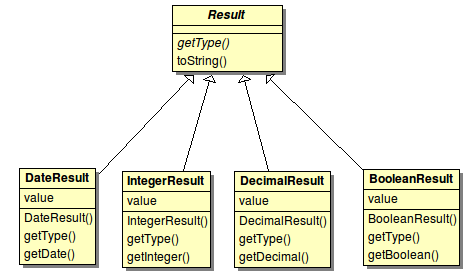
\includegraphics[scale=0.7]{figures/uml_result_classes}
\caption{Wrapping der Rückgabewerte}
\label{figure_result_wrapper}
\end{figure}

Für die Type-Checks wird nur der Rückgabetyp benötigt, da nur der Typ der Statements, aber nicht deren Wert evaluiert wird.


\subsection{Aufbau}

Der Typüberprüfer arbeitet den AST mit einem rekursiven depth-first Ansatz ab und überprüft die Gültigkeit der Datentypen für die Operatoren analog zu den semantischen Typregeln in Tabelle \ref{tbl_semantische_typregeln}. Im Gegensatz zum Interpreter können die Regeln für mehrere Operatoren zusammengefasst werden, da die Rückgabetypen für bestimmte Operatoren den gleichen Regeln unterliegen. 

Beispielsweise können die binären booleschen Operatoren AND und OR nur Operanden des Typs BOOLEAN verarbeiten(Funktion \texttt{checkBinaryBoolean} in Listing \ref{listing_check_binary_boolean}). Liefert einer der Kindknoten einen anderen Typ zurück, wird eine Exception geworfen. Wenn beide Kindknoten gültige Werte liefern, wird wie erwartet der Datentyp BOOLEAN zurückgegeben.

\begin{lstlisting}[float = htbp,caption={Typüberprüfung der binären booleschen Operatoren},label=listing_check_binary_boolean]
private ResultType checkBinaryBoolean(Tree node)
                                 throws FXLException {
	ResultType leftType = check(node.getChild(0));
	ResultType rightType = check(node.getChild(1));
	if (!leftType.equals(ResultType.BOOLEAN)) {
		throw ExceptionFactory.getException(201,
				FXLParser.tokenNames[node.getType()],
				leftType.name());
	} else if (!rightType.equals(ResultType.BOOLEAN)) {
		throw ExceptionFactory.getException(201,
				FXLParser.tokenNames[node.getType()],
				rightType.name());
	}
	return ResultType.BOOLEAN;
}
\end{lstlisting}	

Wie in Tabelle \ref{tbl_semantische_typregeln} ersichtlich, kann der Typ des Rückgabewertes auch von den Typen der Operanden abhängen. Auch die Typen von Variablen und Funktionen werden vom Typüberprüfer evaluiert. Variablenprovider und der Functionmanager bieten dafür entsprechende Methoden an (Abschnitt \ref{section_implementierung_variablen_und_funktionen}).

Normalerweise wäre es von Vorteil, wenn der Typüberprüfer die Überprüfung nach einem gefundenen Fehler fortsetzt, um mehrere Fehler in einem Durchgang melden zu können. In diesem Fall wird darauf verzichtet, da davon ausgegangen wird, das der Anwender kein geübter Programmierer ist, der mit mehreren Fehlermeldungen gleichzeitig umgehen kann.

\section{Variablen und Funktionen}
\label{section_implementierung_variablen_und_funktionen}

Variablen und Funktionen sind in FXL Konzepte, die nicht innerhalb der Sprache definiert werden, sondern in eigenen Komponenten, auf die der Interpreter bzw. Typüberprüfer zugreifen kann (Abbildung \ref{figure_dsl_overview}). 

\begin{figure}[h]
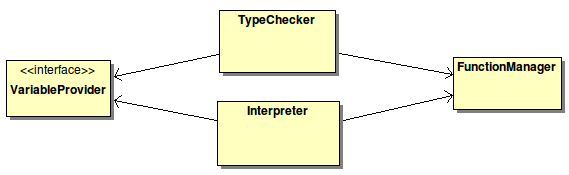
\includegraphics[scale=0.7]{figures/uml_dsl_overview}
\caption{Abhängigkeiten der DSL Implementierung}
\label{figure_dsl_overview}
\end{figure}



\subsection{Variable Provider}

Der Variable Provider ist eine optionale Komponente, der nur dann notwendig ist, wenn der Interpreter versucht, Ausdrücke mit Variablen zu evaluieren. Wie der Name nahelegt, ist dieser für das Lookup der Variablen bzw. deren Typ zuständig. Der Variable Provider ist als einfaches Interface mit zwei Methoden definiert, das abhängig von tatsächlichen Einsatzzweck der DSL implementiert werden kann.

Das Interface definiert zwei Methoden:

\begin{itemize}

	\item \texttt{ResultType lookupType(String name)}: Diese Methode wird vom Typ\-über\-prü\-fer verwendet und überprüft, ob die Variable vorhanden ist, und gibt, falls dies der Fall ist, den Datentyp derselben zurück.
	
	\item \texttt{Result lookup(String name)}: Die lookup-Methode überprüft ebenfalls, ob die Variable vorhanden ist und gibt den Wert der Variable in einer vom Datentyp abhängigen Wrapperklasse (siehe Abbildung \ref{figure_result_wrapper}) zurück.
		
\end{itemize}

Je nach Einsatzgebiet und Implementierung kann das Interface dazu verwendet werden Klassen zu erstellen, die Variablen aus einer simplen Hashmap, einer Datenbank, oder aus anderen Formularfeldern auslesen und an den Interpreter bzw. Typüberprüfer weitergeben.

\subsection{Functionmanager}

Der Functionmanager ist im Gegensatz zum Variable Provider fest in FXL integriert. Um Funktionen hinzuzufügen, können Java-Klassen, die entsprechend annotierte Methoden enthalten, erstellt werden. Der Interpreter enthält Methoden zum Hinzufügen und Entfernen socher Containerklassen. 

Beim ersten Methodenaufruf oder Typcheck werden alle Functioncontainer auf entsprechend annotierte Methoden gescannt, die dann in einer Hashmap gespeichert werden.

\subsubsection{Typüberprüfung}

Bei der Typüberprüfung während der semantischen Analyse muss überprüft werden, ob der Rückgabetyp sowie die Typen der Argumente im DSL-Statement auch den tatsächlich definierten Typen entsprechen oder mit diesen Kompatibel sind. Um dies im Typüberprüfer erledigen zu können, wird die Signatur der Methode abgefragt. Die Signatur einer Funktion besteht aus dem Namen, dem Rückgabetyp und den Typen der Argumente in der korrekten Reihenfolge\footnote{vgl. auch die Problemstellung der Impliziten Typumwandlung, Abschnitt \ref{section_design_funktionen} }.


\subsubsection{Methodenaufruf}

Beim Aufruf einer Funktion in der FXL wird deren Name sowie, wenn vorhanden, die Argumente an den Functionmanager übergeben. Dieser liest die tatsächlichen Werte aus den übergebenen Wrapper-Objekten aus und versucht, die Java-Methode, die der FXL-Funktion zugeordnet ist, mit den ausgelesenen Wertenaufzurufen.

Wenn der Methodenaufruf erfolgreich war, wird der Rückgabewert wieder in einen \texttt{Result}-Untertyp gewrappt und an den Interpreter zurückgegeben. Wenn der Methodenaufruf nicht erfolgreich war, wird eine entsprechende Exception geworfen\footnote{vgl. Fehlercodes in Tabelle \ref{tbl_ausfuhrungsfehler} \nameref{tbl_ausfuhrungsfehler}}.

\section{Interpreter}
\label{design_interpreter}

Wie der Typüberprüfer muss der Interpreter den AST abarbeiten um Statements zu evaluieren. Dazu wird ein depth-first Ansatz gewählt, der rekursiv zuerst den jeweiligen Unterausdruck eines AST-Knotens auswertet.

Eine Besonderheit sind null-Werte. Diese treten auf, wenn ein referenziertes Formularelement noch nicht ausgefüllt wurde. Wenn der Interpreter beim abarbeiten eines AST auf ein \texttt{Result}-Objekt mit Wert \texttt{null} trifft, wird das gesamte Statement mit \texttt{null} evaluiert. Eine detaillierte Erklärung über den Ablauf der Evaluierung im Zusammenhang mit Formularen wird in Abschnitt \ref{implementierung_daten_eingabe} gegeben.

\section{Fehlerbehandlung}

Die Fehlerbehandlung erfolgt wie in Java üblich über Exceptions. Als Grundtyp wird die abstrakte Klasse FXLException definiert. Von ihr leiten sich die konkreten Exceptionklassen \texttt{FXLSyntaxException}, \texttt{FXLSemanticException}, \texttt{FXLRuntimeException} und \texttt{FXLImplementationException} ab, die den in Abschnitt \ref{section_design_fehlerbehandlung} definierten Arten von Fehlern entsprechen. Die Fehlerklassen sind, im Gegensatz zu den anderen Klassen der DSL, mit dem Prefix `FXL' versehen, um eine Verwechslung mit vorhandenen Java-Klassen (z.B. \texttt{java.\-lang.\-Runtime\-Exception}) zu verhindern. Eine Exception enthält einen Fehlercode, eine textuelle Fehlermessage und optional ein oder mehrere Objekte, die zusätzliche Informationen zum Fehler beinhalten (vgl. Abbildung \ref{abb_exception_hierarchie}).

\begin{figure}[ht]
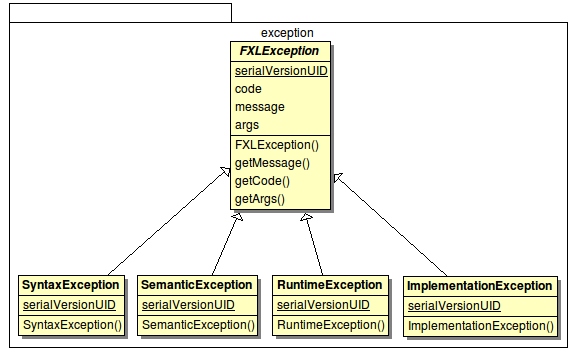
\includegraphics[scale=0.7]{figures/uml_exception_hierarchy}
\caption{Exception Hierarchie}
\label{abb_exception_hierarchie}
\end{figure}


\chapter{Test}
\label{chapter_test}

Auch wenn die Phase Test in dieser Arbeit am Ende des Entwicklungsprozesses angeführt wird, ist sie keineswegs als letzte Phase während der Entwicklung selbst zu sehen. Vielmehr ist das Erstellen und wiederholte Durchführen von Testfällen integrativer Bestandteil des Entwicklungsprozesses.

In diesem Kapitel werden zuerst die theoretischen und methodischen Grundlagen aufgearbeitet und eine Übersicht geboten. In weiterer Folge wird das Vorgehen bei der Entwicklung der FXL erläutert.



\section{Grundlagen}

Das Testen von Software ist genau wie die entstehenden Produkte sehr facettenreich. Spillner und Linz definieren den Begriff Testen wie folgt:

\begin{myquote}
Unter dem Test von Software verstehen wir die stichprobenartige Ausführung eines Testobjekts, die zu dessen Überprüfung dienen soll. Dazu müssen die Randbedingungen für die Ausführung des tests festgelegt sein. Über einen Vergleich zwischen Soll- und Istverhalten wird bestimmt, ob das testobjekt die geforderten Eigenschaften erfüllt.\cite{SpLi10}
\end{myquote}

\subsection{Grundsätzliche Einteilung von Tests}

Softwaretests lassen sich nach diversen Kriterien einteilen. In diesem Abschnitt erfolgt eine Übersicht über verschiedene Arten und Vorgehensweisen von Softwaretests.

\subsubsection{Granularität von Tests}

Tests können auf verschiedenen Ebenen durchgeführt werden. Je nach Literatur werden meistens die folgenden drei Levels unterschieden\footnote{vgl. \cite{ISTQB1}}:

\begin{itemize}
  \item Komponententest: Testet einen kleineren Teil (Klasse, Modul, Programm etc.) eines Softwaresystems, der seperat testbar ist.
  \item Integrationstest: Testet die Integration und Interaktionen zwischen verschiedenen Teilen eines Systems.
  \item Systemtest: Testet das Verhalten eines kompletten Systems und sollte deshalb auch in einer dem Produktivsystem ähnlichen oder gleichen Umgebung durchgeführt werden.
\end{itemize}

Zusätzlich können noch weitere Arten wie Akzeptanztests, Abnahmetests, Regressionstests etc. identifiziert werden.

In diesem Teil der Arbeit ist vor allem der Komponententest von Bedeutung. Komponententests können wiederum in White- und Blackbox Tests eingeteilt werden. Bei Whitebox-Tests werden die Tests aufgrund der bekannten inneren Struktur einer Komponente designt. Blackbox-Tests testen eine Komponente auf ein spezifiziertes Verhalten.


\subsubsection{Arten von Tests}

Softwaretests können nach diversen Kriterien eingeteilt werden. Eine grundsätzliche Einteilung ist jene in \emph{Funktionale} und \emph{Nichtfunktionale Tests}. Funktionale Tests überprüfen ``was'' die Software macht. Das heißt, ob die Funktionen den spezifizierten Anforderungen entsprechen. Nichtfunktionale Tests untersuchen ``wie'' die Software arbeitet. Das beinhaltet diverse Qualitätskriterien wie Performance, Wartbarkeit, Portierbarkeit, Sicherheit, Usability etc.

Tests können auch nach dem Grad der Automatisierung eingeteilt werden. Hier wird zwischen manuellen und automatisierten Tests unterschieden. Manuelles Testing ist vor allem für graphische User Interfaces und Software auf mobilen Endgeräten relevant.

Weiters können Tests auch durch die Ausführung der Software unterschieden werden. Tests, bei denen die Software nicht zur Ausführung kommt, werden \emph{statische Tests} genannt. Statische Methoden sind vor allem Code Reviews, die manuell von Entwicklern durchgeführt werden, und Tools zur Codeanalyse. Wenn die Software beim Testing zur Ausführung kommt, spricht man von \emph{dynamischen Tests}.




\section{Test der DSL}

Die FXL ist eine Abgeschlossene Library und wird daher auf Komponentenebene getestet. Der entwickelte Interpreter hat ein sehr genau spezifiziertes Verhalten. Die Evaluierung von Formeln ist deterministisch und damit sehr gut testbar, da für eine Formel ein, von den Eingabewerten abhängiges, eindeutiges Ergebnis erwartet werden kann. Die Tests sind als Blackbox Tests konzipiert, da die Implementierung nicht für das Ergebnis relevant ist.

\subsection{Testfälle}

Das Erstellen von Testfällen für die FXL erweist sich als sehr umfangreich, weil der Funktionsumfang relativ groß ist. Die Testfälle müssen

\begin{itemize}

 \item Operatoren,

 \item Datentypen,

 \item Variablen,

 \item Funktionen,

 \item und Kombinationen der obigen mit Klammerausdrücken
\end{itemize}

abdecken. Zusätzlich muss beachtet werden, dass einige Operatoren überladen sind und daher mit verschiedenen Kombinationen von Datentypen getestet werden (siehe Beispiel in Listing \ref{listing_example_test_case}). Auch verschiedene Eigenschaften der Sprache wie Kommutativ- oder Assoziativgesetz sowie die Rangfolge der Operatoren werden getestet.

Weiters müssen Testfälle mit fehlerhaften Statements erstellt werden, um das korrekte Verhalten der Sprache in Hinsicht auf Fehlermeldungen zu prüfen.

\begin{lstlisting}[caption={Beispielhafter Testfall für den Multiplikations-Operator \texttt{*}. Zuerst wird ein Statement mit Ganzzahlen ausgeführt, dann eine Multiplikation mit 0, eine Multiplikation zweier Gleitkommazahlen und dann zwei Multiplikationen mit je einer Gleitkomma- bzw. Ganzzahl.},label=listing_example_test_case]
@Test
public void testSimpleMult() throws FXLException {

	expr = "=1*1";
	interpreter.setExpression(expr);
	result = interpreter.evaluate();
	assertEquals(new Long(1),((IntegerResult)result).getInteger());

	expr = "=1*0";
	interpreter.setExpression(expr);
	result = interpreter.evaluate();
	assertEquals(new Long(0), ((IntegerResult)result).getInteger());

	expr = "=0.5*0.5";
	interpreter.setExpression(expr);
	result = interpreter.evaluate();
	assertEquals(new BigDecimal(0.25).setScale(4), ((DecimalResult)result).getDecimal());

	expr = "=0.5*50";
	interpreter.setExpression(expr);
	result = interpreter.evaluate();
	assertEquals((new BigDecimal(25.0)).setScale(4), ((DecimalResult)result).getDecimal());

	expr = "=50*0.5";
	interpreter.setExpression(expr);
	result = interpreter.evaluate();
	assertEquals((new BigDecimal(25.0)).setScale(4), ((DecimalResult)result).getDecimal());
	}
\end{lstlisting}

\subsection{Testdaten}

Um sinvolle Tests zu erstellen, ist es notwendig gute Testdaten zu finden, mit denen die Tests ausgeführt werden. Es gibt verschiedene Verfahren, um Testdaten für Testfälle zu bestimen.

Für System-, Integrations- und Abnahmetests eignen sich definierte Anwendungsfälle, die im Test in Hinsicht auf funktionale und nichtfunktionale Kriterien ausgeführt werden können.

Auf Komponentenebene sind die klassischen Verfahren die Äquivalenzklassenbildung und Grenzwertanalyse. Die Äquivalenzklassenbildung versucht, Klassen von Testwerten zu bestimmen, die ein bestimmtes Verhalten hervorrufen. Mit Hilfe der Grenzwertanalyse werden Werte ermittelt, die die Fallunterscheidungen an den Grenzen der Äquivalenzklassen untersuchen sollen. Die Grenzwertanalyse kann also als Erweiterung der Äquivalenzklassenbildung gesehen werden.



\subsection{Testdriven Development}

Die Technik des Testdriven Development (TDD) erfordert vom Entwickler, automatisierte Tests bereits vor der Implementierung zu erstellen. Dies führt dazu, dass manche Aspekte, die während der Programmierung unter Umständen nicht beachtet werden, bereits durch Testfälle abgedeckt werden. Ein weiterer Vorteil ist, dass die Software von vorn herein ein testbares Design erhält, das umständliche Änderungen für Tests im Nachhinein vermeidet.

Die Aufgabenstellung der DSL eignet sich hervorragend für die Testgetriebene Entwicklung durch Unit-Tests. Die Statements, die vom Interpreter verarbeitet werden sollen, liegen von vornhinein fest. Die Statements bestehen aus diversen Kombinationen von Operatoren mit Werten verschiedener Datentypen. Diese Kombinationen sollen teilweise durch Klammerung verändert werden und in ihrer Länge variieren.









\part{Integration in ein existierendes System}
\label{part_integration}
Im dritten Teil der Arbeit wird die im zweiten Teil entwickelte DSL in eine bestehende medizinische Dokumentationssoftware eingebunden.

Die Implementierung der FXL ist eine eigenständige Java-Bibliothek und damit unabhängig vom Zielsystem. Um die Bibliothek zu verwenden, muss evaluiert werden, wie und wo die Schnittstellen integriert werden können und wie die Interaktion mit dem Endbenutzer des Systems gestaltet wird.  

Zuerst wird das Studiensystem SPICS beschrieben, um dem Leser der Arbeit eine Übersicht über das System zu bieten. Es soll helfen, das not\-wen\-dige Verständnis für den Nutzen der FXL zu erzeugen. Danach werden die einzelnen Aspekte und Überlegungen bei der Integration vorgestellt.

\chapter{Systembeschreibung}
\label{chapter_systembeschreibung}

Dieses Kapitel erläutert den Aufbau der Dokumentationssoftware SPICS, um ein Verständnis für die Anwendung der Form Expression Language in der Implementierung herzustellen. Neben der Beschreibung des technischen Aufbaus werden auch die konkreten Anwendungsfälle der FXL erklärt, um nachvollziehen zu können, an welchen Stellen in den Workflow eingegriffen wird.


\section{SPICS}

SPICS (Secure Platform for Integrating Clinical Services) ist ein Projekt der  Forschungsgruppe Industrial Software der TU Wien. Die Software ist eine Webanwendung, die Krankenhäusern, Ärzten und anderen Spezialisten -- unter Berücksichtigung des Datenschutzgesetzes -- den gemeinsamen Zugriff auf Daten für medizinische Studien er\-mög\-licht. 

Die SPICS Plattform bietet die Möglichkeit, für verschiedene medizinische Fachbereiche bzw. Anforderungen individuelle Eingabemasken zu erstellen. Dafür können aus unterschiedlichen Formularfeldern flexibel benutzerdefinierte Formulare erstellt werden. Weitere Features sind der Import und Export der gesammelten Studiendaten, um diese mit externen Statistik-Tools auszuwerten. Dabei ist zu beachten, dass die Anonymität der Patienten und Studienteilnehmer gesichert ist, da die medizinischen Daten nur pseudonymisiert abgelegt werden.


\section{Workflow}
\label{section_systembeschreibung_workflow}

Um die Integration in das Dokumentationssystem zu verstehen, werden zuerst die wichtigsten Anwendungsfälle erörtert, um zu veranschaulichen, wo die DSL die Arbeit mit den Daten erleichtern kann. Zuerst wird der typische Ablauf anhand eines Beispiels durchgespielt, um danach zu erläutern, wo die FXL den Workflow verbessern kann.

SPICS enthält ein umfassendes Rollen- und Berechtigungssystem. Die für diese Arbeit essentiellen Rollen sind jene des Administrators und des Contributors. Administratoren sind berechtigt, Formulare zu erstellen und zu bearbeiten. Contributoren sind hingegen jene Benutzer, die Daten in die Formulare eingeben.

\subsection{Workflow anhand eines Beispiels}
\label{subsection_workflow_beispiel}


Um den typischen Ablauf zu verdeutlichen, werden die maßgeblichen Anwendungsfälle für ein beispielhaftes Formular angeführt. Im darauf folgenden Abschnitt wird eruiert, wo die FXL in diesen Ablauf eingreift, um den Endanwender bei der Eingabe der medizinischen Daten zu unterstützen.

Natürlich enthält ein so aufwändiges System wie SPICS neben dem \mbox{hier} vorgestellten auch zahlreiche weitere Workflows, etwa für Datenexport und -import, Benutzerverwaltung, Konfiguration und Terminverwaltung. Auf diese soll hier jedoch nicht eingegangen werden, um den Focus auf das Thema der Arbeit nicht zu verlieren.

Der Workflow soll am Beispiel eines Formulars gurchgegangen werden, in dem die Veränderung des Body-Mass-Index (BMI) eines Patienten dokumentiert wird. Ein Arzt (bzw. aus Software-Sicht: der Endanwender) soll also in der Lage sein, den BMI eines Patienten an verschiedenen Tagen zu dokumentieren. Abbildung \ref{abb_workflow_formular_ausfuellen} auf Seite \pageref{abb_workflow_formular_ausfuellen} zeigt das fertige Formular, in das die Daten eingegeben werden können.

Das in den folgenden Schritten erstellte Formular soll im gesamten zweiten Teil der Arbeit als Beispiel dienen, da es einerseits einfach nachzuvollziehen ist und andererseits einige grund\-sätz\-liche Konzepte und Überlegungen beinhaltet, die im weiteren Verlauf der Arbeit erläutert werden\footnote{vgl. Abschnitt \ref{implementierung_dsl_eingabe}  \nameref{implementierung_dsl_eingabe} sowie Abschnitt \ref{implementierung_daten_eingabe} \nameref{implementierung_daten_eingabe}}.

\subsection{Use Cases}

\subsubsection{Erstellen eines neuen Formulars}

Der erste Schritt im Workflow ist das Erstellen eines neuen Formulars. Es ist zuerst ein Titel zu vergeben, sowie einzustellen, ob das Formular pro Patient einmal oder mehrmals ausfüllbar ist. Diese Unterscheidung ist not\-wen\-dig, da manche Daten nur einmal zu erheben sind (z.B. Stammdaten, oder Daten zur Geburt eines Patienten). Oft ist es allerdings auch not\-wen\-dig (wie im oben beschriebenen Beispiel), ein Formular für einen Patienten mehrmals auszufüllen, etwa um einen zeitlichen Verlauf zu dokumentieren.
 
\begin{figure}[h]
\begin{center}
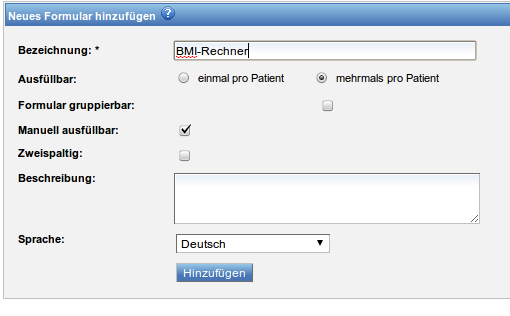
\includegraphics[scale=0.5]{figures/workflow_neues_formular}
\caption{Erstellen eines neuen Formulars}

\label{abb_workflow_neues_formular}
\end{center}
\end{figure}

Zu\-sätz\-lich können auch weitere Parameter angegeben werden (Abbildung \ref{abb_workflow_neues_formular}), die beispielsweise das Layout oder die Sprache betreffen. Diese Einstellungen haben allerdings für das Beispielformular keine Relevanz.

Das Ergebnis dieses Schrittes ist ein leeres Formular, das nun mit einer beliebigen Anzahl und Anordnung von Formularelementen gefüllt werden kann.

\subsubsection{Editieren eines Formulars}

Wenn ein Formular neu erstellt wurde (bzw. wenn es bereits existiert oder importiert wurde) kann es editiert werden. Darunter wird das Anlegen, Verändern und Löschen von Formularelementen verstanden. Zu\-sätz\-lich werden Formularelemente in Gruppen zusammengefasst, um eine übersichtliche Struktur zu schaffen.

Manche Formularelemente können mit einfachen Constraints belegt werden. So kann bei einem Datumsfeld der Datumsbereich (von-bis) ausgewählt werden. Bei Textfeldern kann der Datentyp insofern festgelegt werden, als dass zwischen \emph{Text}, \emph{Ganzzahl} und \emph{Kommazahl} unterschieden wird. Bei den beiden lezteren ist wiederum ein Constraint möglich, der den Wertebereich einschränkt. Außerdem kann für jedes Formularelement festgelegt werden, ob es ein Pflichtfeld ist.

Für das Beispielformular wird zuerst eine Gruppe mit dem Namen `BMI-Rechner` erstellt. In dieser Gruppe werden nun drei Textfelder
für das Kör\-per\-ge\-wicht, die Kör\-per\-grö\-ße und den BMI angelegt. Zu\-sätz\-lich wird noch eine Checkbox mit dem Titel `Adipositas` hinzugefügt.

\subsubsection{Auswählen eines Patienten}

Der nächste Schritt ist die Auswahl eines Patienten, für den das Formular ausgefüllt werden soll. Hier findet ein Wechsel der Rolle des Benutzers vom Administrator zum Contributor statt. Waren für die bisherigen Schritte Berechtigungen zum Erstellen und Editieren von Formularen not\-wen\-dig, so ist ab nun lediglich die Berechtigung zum Ausfüllen der Formulare erforderlich. 

Zunächst wird ein Patient anhand seines Synonyms aus der Liste aller Patienten ausgewählt. Auf der Übersichtsseite für einen Patienten sind alle bereits ausgefüllten Formulare aufgelistet. Soll ein neues Formular hinzugefügt werden, muss der Name des Formulars ausgewählt werden. 

\subsubsection{Ausfüllen eines Formulars}

\begin{figure}[h]
\begin{center}
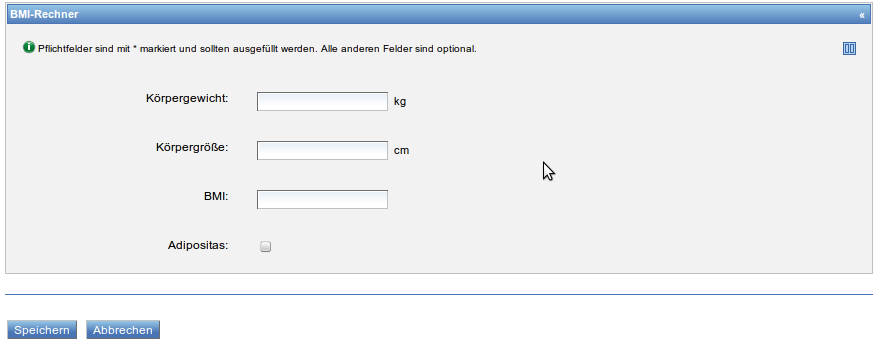
\includegraphics[scale=0.5]{figures/workflow_formular_ausfuellen}
\caption{Ausfüllen des neuen Formulars}

\label{abb_workflow_formular_ausfuellen}
\end{center}
\end{figure}

Wurde auf der Übersichtsseite eines Patienten das Formular `BMI-Rechner` ausgewählt, erscheint nun das in den vorigen Schritten erstellte Formular (Abbildung \ref{abb_workflow_formular_ausfuellen}). Der Endanwender kann nun die ent\-sprech\-enden Daten in die dafür vorgesehenen Felder eingeben. Der BMI muss hier mithilfe eines Taschenrechners oder Tools berechnet werden. Ist sein Wert größer 30, so handelt es sich laut WHO um Fettleibigkeit (Adipositas)\footnote{ vgl. \cite{Who00} }. In diesem Fall sollte die Checkbox `Adipositas` angeklickt werden.



\section{Architektur und Technologien}

Dieser Abschnitt enthält einen Überblick über die Softwarearchitektur und die verwendeten Technologien, um die Integration der Form Expression Language aus technischer Sicht nachvollziehen zu können.


\subsection{Architektur}

Die Architektur von SPICS ist als klassische 3-Tier Applikation mit gra\-phisch\-er Benutzeroberfläche, Programmlogik und Datenzugriffsschicht ausgeführt (Abbildung \ref{abb_spics_architektur}). 

\begin{figure}[h]
\begin{center}
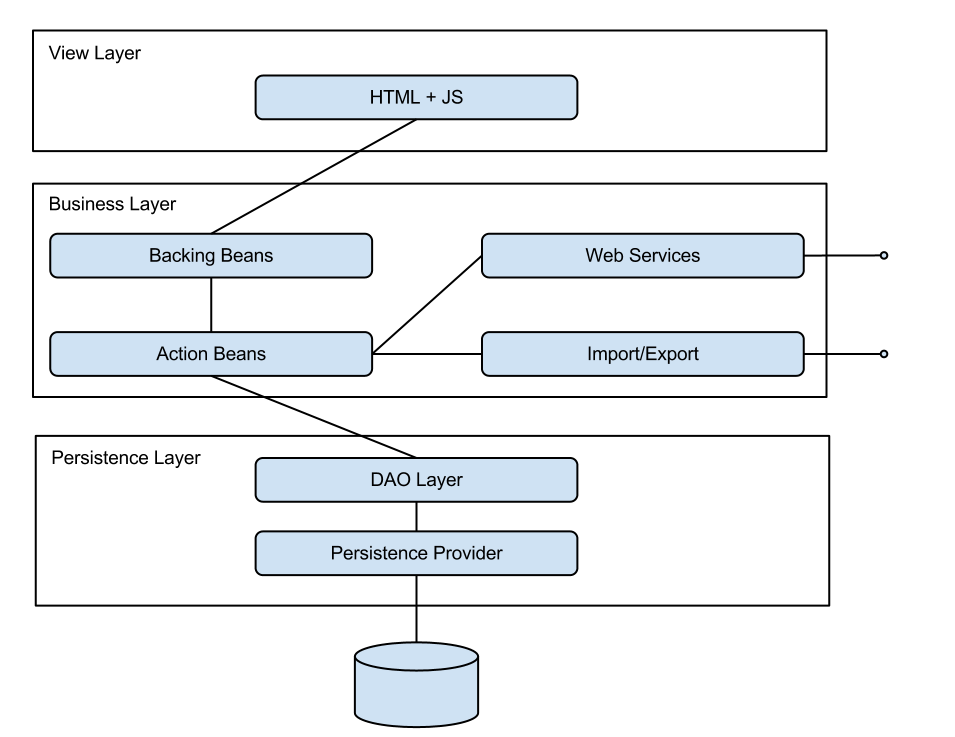
\includegraphics[scale=0.4]{figures/spics_architektur_neu}
\caption{Übersicht über die 3-Tier Architektur}

\label{abb_spics_architektur}
\end{center}
\end{figure}

Die Benutzerschnittstelle ist eine Webapplikation, die auf die Backing Beans der Logikschicht zugreift. Unterstützt wird die GUI durch Java\-Script-basierte Widgets wie z.B. Date Picker. Wo möglich bzw. sinnvoll werden AJAX-Calls verwendet, um den Workflow flüssiger zu gestalten.

Der Kern der Software besteht aus Komponenten, die die Programmlogik enthalten. Diese sind einerseits Backing Beans, deren Attribute an die Benutzerschnittstelle gebunden werden, andererseits Action Beans, in denen Daten verarbeitet werden. Zu\-sätz\-lich bietet die Software auch noch eine Webservice-Schnittstelle und Komponenten zum Import und Export von Formularen und medizinischen Daten.

Die Komponenten der Logik-Schicht greifen auf die darunter liegende Datenbank über Data Access Objects (DAOs). Das Datenmodell des Systems wird über objektrelationales Mapping auf die Tabellen der relationalen Datenbank abgebildet.



Eine zusätzliche Besonderheit von SPICS ist die Trennung der persönlichen Patientendaten von den Behandlungsdaten. Diese örtliche Trennung ist not\-wen\-dig, um den Datenschutz der Patienten zu gewährleisten. Das Zusammenführen der perönlichen Daten mit den medizinischen Daten erfolgt erst im Browser des Benutzers. Auf diese Eigenschaft wird hier nicht weiter eingegangen, da sie für die Aufgabenstellung nicht relevant ist. Sie soll aber trotzdem erwähnt werden, da dies ein Key-Feature von SPICS darstellt.

\subsection{Technology Mapping}

Der Kern der Dokumentationssoftware SPICS ist als Java Enterprise Applikation, basierend auf dem Framework Seam ausgeführt. Als Applicationserver wird der JBoss AS verwendet. Auf die darunterliegende PostgreSQL Datenbank wird mittels Hibernate als ORM Mapper zugegriffen.

Verwendete Technologien des Systems:

\begin{itemize}
	\item Java 6
	\item PostgreSQL
	\item JBoss AS 5.1.0.GA
	\item Seam 2.2
	\item JSF 1.2
\end{itemize}



\chapter{Integration}


Im folgenden Kapitel werden die einzelnen Themen der Integration der Form Expression Language in das Studiensystem SPICS präsentiert. Zuerst werden die Anwendungsfälle der FXL in SPICS beschrieben und dargestellt, wo diese die Anwendung und in weiterer Folge das Datenmodell beeinflussen. Danach werden die verschiedenen Aspekte bei der Modellierung von Formularen mit Hilfe der FXL, sowie die Eingabe der Daten in das Studiensystem beschrieben. Zuletzt wird noch auf die Implementierung der Fehlerbehandlung eingegangen, die dem Benutzer Feedback über Probleme und deren Ursachen durch genaue Fehlermeldungen bereitstellt.


\section{Die FXL in SPICS}

Wie der Titel der Arbeit aussagt, soll die Modellierung der Formulare durch die entwickelte domänenspezifische Sprache unterstützt werden. Das zu\-sätz\-li\-che Feature in Hinsicht auf die Modellierung ist, dass die Integration der FXL er\-mög\-licht, die Formularelemente eines individuellen Formulars miteinander in Beziehung zu setzen.

\subsection{Anwendungsfälle}

In der aktuellen Version sind die einzelnen Eingabefelder eines For\-mu\-lars unabhängig voneinander. Eine Eingabe in einem Feld kann den Wert eines anderen Feldes nicht beeinflussen. Der Endanwender muss dafür Sorge tragen, dass die Felder zueinander sinnvolle Werte beinhalten. Wenn der berechnete BMI im Beispielformular größer als 30 ist, sollte der Bearbeiter des Formulars die Adipositas-Checkbox anckecken. Es gibt allerdings in der aktuellen Version des Systems, abgesehen von speziellen Plugins, keine Möglichkeit zu überprüfen, ob die Checkbox korrekt gesetzt wurde.

Es kristallieren sich die folgenden zwei Anwendungsfälle heraus:

\begin{itemize}
  \item Berechnen von Formularfeldern mit \textbf{Formeln}.
  \item Überprüfen von Formularfeldern durch Bedingungen (\textbf{Constraints})\footnote{Die Begriffe Bedingung, Einschränkung und Constraint werden in weiterer Folge für diesem Context synonym verwendet.}
\end{itemize}

\paragraph{Formeln} 

Im BMI-Formular des Beispiels bieten sich zwei Felder für die automatische Berechnung durch eine Formel an. Einerseits natürlich der BMI, der sich aus den Feldern Körpergewicht und Kör\-per\-grö\-ße mit der Formel

\begin{center}
 BMI = Körpergewicht in kg / ( Kör\-per\-grö\-ße in m )$ ^2 $
\end{center}

berechnen lässt. Anderererseits lässt sich aber auch der Wert der Adipositas-Checkbox durch die Formel

\begin{center}
 Adipositas = BMI $ > $ 30
\end{center}

berechnen. Eine Checkbox kann nur zwei Zustände haben: ausgewählt und nicht ausgewählt. Diese Zustände stehen implizit für die booleschen Werte wahr und falsch. Wie in Tabelle \ref{tbl_semantische_typregeln} ersichtlich, geben Vergleichsoperatoren allgemein einen booleschen Wahrheitswert zurück. Der Rückgabewert der Adipositas-Formel kann also verwendet werden, um den Wert der Checkbox ent\-sprech\-end zu setzen.

Allgemein kann also gesagt werden, dass Formeln verwendet werden, um den Wert eines Formularelements (in Abhängigkeit zu anderen Formularelementen) zu verändern.

\paragraph{Constraints}

Im Beispielformular gibt es auch Einschränkungen, was die Gültigkeit bzw. Sinnhaftigkeit der Eingabegrößen betrifft. Sowohl die Kör\-per\-grö\-ße, als auch das Körpergewicht muss größer als null sein, da negative Werte natürlich nicht sinnvoll sind. Ein weiterer Constraint kann sein, dass ein Feld ausgefüllt sein muss und daher als Pflichtfeld definiert wird. Diese Einschränkungen hängen allerdings nicht von anderen Formularelementen ab und werden auch, wie in Abschnitt \ref{subsection_workflow_beispiel} erwähnt, vom momentanen System unterstützt.

Eine Erweiterung der Überprüfung wäre, wenn andere Formularfelder in die Überprüfung mit einbezogen werden könnten. Angenommen eine Studie möchte die Nachbehandlung einer Operation dokumentieren und erstellt ein Formular, in das zusätzlich zu den medizinischen Daten der Operationstermin, sowie der Termin der Nachbehandlung eingetragen wird. In diesem Fall ist es not\-wen\-dig, dass der Termin der Nachbehandlung erst nach dem Operationstermin stattfindet. Es handelt sich also um eine Bedingung, die vom Wert eines anderen Formularfeldes abhängig ist. 

Es muss also eine Formel definiert werden, die den Constraint beschreibt. zusätzlich muss diese Formel einen booleschen Wahrheitswert als Rückgabetyp haben, da ja überprüft werden soll, ob der Wert eines Feldes gültig ist (true) oder nicht (false). Für das obige Beispiel könnte die Formel wie folgt aussehen:

\begin{center}
 Constraint = Nachbehandlung $ > $ Operationstermin
\end{center}

Allgemein kann also gesagt werden, dass Constraints verwendet werden, um den Wert eines Formularelements (in Abhängigkeit zu anderen Formularelementen) zu überprüfen.

Ob ein Formular trotz fehlgeschlagenem Constraint abgespeichert werden darf, liegt nicht im Einfluss dieser Arbeit. SPICS bietet eine Kon\-fi\-gu\-ra\-tions\-op\-tion, die bestimmt, ob Formulare abgespeichert werden dürfen, wenn die Validierung fehlschlägt. Je nach Einsatzzweck können Constraints also das Speichern verhindern, oder nur als Warnung dienen.


\subsection{Anknüpfungspunkte}

Da nun der Zweck der Form Expression Language in der konkreten Anwendung klar ist, stellt sich die Frage, wo nun im oben angeführten Workflow Än\-der\-ung\-en vorgenommen werden müssen, um die Funktionalität der DSL in die Anwendung zu integrieren. Es ist klar, dass die Statements der DSL einerseits eingegeben\footnote{vgl. Abschnitt \ref{implementierung_dsl_eingabe}  \nameref{implementierung_dsl_eingabe}} und andererseits ausgeführt\footnote{vgl. Abschnitt \ref{implementierung_daten_eingabe} \nameref{implementierung_daten_eingabe}} werden müssen. 

Die Statements der FXL werden bei der Modellierung des Formulars eingegeben. Hier erfolgt in erster Linie die Syntaxüberprüfung und die semantische Analyse mit der ent\-sprech\-enden Fehlerbehandlung. Weiters müssen auch andere Dinge wie zyklische Abhängigkeiten überprüft werden (siehe Abschnitt \ref{implementierung_zyklenueberpruefung}). Die Aus\-führ\-ung der Statements erfolgt beim Ausfüllen der Daten in ein Formular, wenn es Berechnungen durch Formeln enthält. Hier ist vor allem die Reihenfolge der Berechnungen interessant, da natürlich Felder, von denen ein anderes Feld abhängt, zuerst berechnet werden müssen (siehe Abschnitt \ref{implementierung_integration_reihenfolge}).


\section{Sicherheit und Stabilität}

In diesem Abschnitt soll auf einige Fragen der Sicherheit und Stabilität der FXL, sowie deren Integration in SPICS eingegangen werden. Unter Stabilität wird die Fähigkeit des Systems verstanden, auf unvorhergesehene Eingaben angemessen, also nicht durch Systemabsturz sondern entsprechende Fehlermeldungen, zu reagieren. 

Beim Entwurf der FXL wurde darauf geachtet, die Stabilität der Anwendung, in der diese integriert wird, nicht zu beeinflussen. Fehlerhafte Scripts, die z.B. Endlosschleifen enthalten, können durch das Design der Sprache ausgeschlossen werden, da der Interpreter nur einzelne, in der Syntax der Sprache definierte, Ausdrücke verwerten kann (vgl. Abschnitt \ref{section_java_scripting}). Da jedoch Funktionen über den Functionmanager Java-Methoden aufrufen\footnote{vgl. Abschnitt \ref{design_implementierung_functionmanager}}, be\-steht die Möglichkeit von Fehlern im Java Code. Diese Java-Methoden müssen jedoch der FXL explizit zur Verfügung gestellt werden, beliebige Methodenaufrufe sind nicht möglich. Da es keine angemessene Möglichkeit zur absoluten Absicherung von Methodenaufrufen, etwa in Hinblick auf Endlosschleifen, gibt\footnote{Methodenufrufe in einer Art ``Sandbox'' auszuführen, ist innerhalb einer Java Virtual Machine (JVM) nicht möglich, da man das Schließern von Threads nicht sauber erzwingen kann. Eine Möglichkeit, diese Einschränkung zu umgehen, könnte das Starten einer zusätzlichen JVM in einem separaten Prozess darstellen.}, muss den Methoden, die dem Functionmanager zur Verfügung gestellt werden, vertraut werden. Viele Fehler, wie etwa Endlosrekursion, können mit in der FXL Implementierung abgefangen und auf entsprechende \texttt{FXLException}s gemappt werden.


Um die Stabilität der Ausführung gewährleisten, müssen die voneinander abhängigen Formeln eines Formulars auf Zyklenfreiheit überprüft werden um ``Endlosevaluierungen'' zu vermeiden. Diese Überprüfung wird in Abschnitt \ref{implementierung_zyklenueberpruefung} beschrieben. Um die Integrität der Daten zu sichern, müssen voneinander abhängige Felder in der korrekten Reihenfolge ausgeführt werden (Abschnitt \ref{implementierung_integration_reihenfolge}).

Eine weitere Möglichkeit, die Sicherheit und Stabilität zu gefährden, ist das direkte Editieren der Scripts in der Datenbank. Wie in Abschnitt \ref{implementierung_datenmodell} erläutert, werden die Formeln und Constraints in der Datenbank zu dem jeweiligen Formularelement gespeichert. Wer Zugriff auf die Datenbak hat, kann demnach auch fehlerhafte Statements in ein Formular einschleusen. Eine weitere Fehlerquelle kann der Import von Formularen darstellen. Beim Import wird das Formular deshalb auf Zyklenfreiheit und inkorrekte Statements überprüft. In beiden Fällen muss allerdings den Benutzern mit entsprechenden Rechten, vertraut werden.


Vor jeder Ausführung eines Statements im Interpreter durchläuft dieses alle Analyseschritte einer Language Application (siehe \ref{theorie_language_applications}). Zuerst wird der Abstract Syntax Tree erstellt. Dieser Vorgang impliziert die lexikalische und syntaktischen Analyse. Danach wird ein Typecheck auf dem AST ausgeführt, was der semantischen Analyse entspricht. Erst danach wird das Statement interpretiert. Treten in einer Phase Fehler auf, wird eine entsprechende Fehlermeldung zurückgegeben (siehe Abschnitt \ref{section_design_fehlerbehandlung}). Die ersten zwei Schritte werden natürlich für jedes Statement nur einmal ausgeführt, bei jedem weiteren Aufruf wird der bereits bestehende und überprüfte AST abgearbeitet. 




\section{Än\-der\-ung\-en im Datenmodell}
\label{implementierung_datenmodell}

Die individuell zusammengestllten Formulare werden durch drei Klassen abgebildet, die per JPA in der Datenbank persistiert werden. Wie in Abbildung \ref{abb_uml_datenmodell} ersichtlich, besteht ein Formular aus einer oder mehreren Gruppen von Formelementen. Eine Gruppe wiederum besteht aus den Klassen der einzelnen Formelemente (Textfield, Checkbox etc.). Da die Variablen, Formeln und Constraints für die einzelnen Formularelemente ebenfalls ge\-spei\-chert werden müssen, wurde eine neue Klasse \texttt{DslAttribute} hinzugefügt.

\begin{figure}[ht]
\begin{center}
 
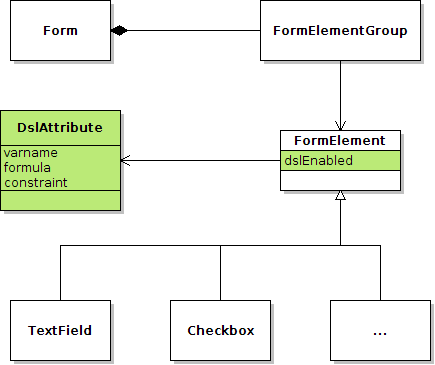
\includegraphics[scale=0.7]{figures/uml_datenmodell_neu}
\end{center}

\caption{Datenmodell der Formulare. Die grün gefärbten Bereiche sind jene, die im Zuge der Integration verändert wurden.}
\label{abb_uml_datenmodell}
\end{figure}

Jedes Formelement enthält eine boolesche Variable namens dslEnabled. Dieses Flag bestimmt, ob der Untertyp der Klasse Formelement zum Berechnen durch die FXL geeignet ist. Wenn ja, bekommt jedes Objekt dieses Formelements einen Verweis auf ein Objekt vom Typ DslAttribute. Die Klasse DslAttribute selbst enthält alle Informationen, die ein DSL-enabled Feld benötigt: den Variablennamen, eine Formel und einen Constraint. 

Es gibt zwei Möglichkeiten, die neue Klasse in das Datenmodell einzubinden: Als One-to-one Relation mit einem Foreign Key in einer der Klassen, oder als Embedded Object in der Klasse \texttt{Formelement}. In der ersten Variante wird eine eigene Tabelle für die Klasse \texttt{DslAttribute} erstellt. Über ein Id-Feld, welches zur Klasse hinzugefügt werden muss, wird die neue Tabelle über ein Foreign-Key Feld mit einem Formelement verbunden.

Die zweite Variante, die auch in der Implementierung verwendet wird, verändert lediglich die bestehende Tabelle der Formelemente. Es werden drei Spalten hinzugefügt, die die Attribute der Klasse \texttt{DslAttribute} repräsentieren. Der Vorteil dieser Methode ist, dass eine Tabelle weniger erstellt wird und somit ein Join bei der Abfrage eingespart wird.

\begin{lstlisting}[float = htbp,caption={Embedded DslAttribute },label=listing_dslattribute]
@Embeddable
public class DslAttribute {

  private FormElement formElement;
  
  @Column
  private String variableName;

  @Column
  private String formula;

  @Column
  private String constraintFormula;

  ...
}
\end{lstlisting}


Listing \ref{listing_dslattribute} enthält einen Auszug aus der neu erstellten Klasse, ohne Getter bzw. Setter und den Methoden toString(), hashCode() und equals().

\section{DSL Eingabe}
\label{implementierung_dsl_eingabe}

Die Eingabe des Variablennamens, der Formel und des Constraints erfolgt in der Eingabemaske des jeweiligen Formelements (siehe Abbildung \ref{abb_screenshot_spics_eingabe}). Dazu werden, wenn die DSL für den Typ des Formelements aktiviert ist, dem Eingabeformular drei Textfelder hinzugefügt, die per JSF an die Attribute der Klasse DslAttribute gebunden werden.


\begin{figure}[h]
\begin{center}
 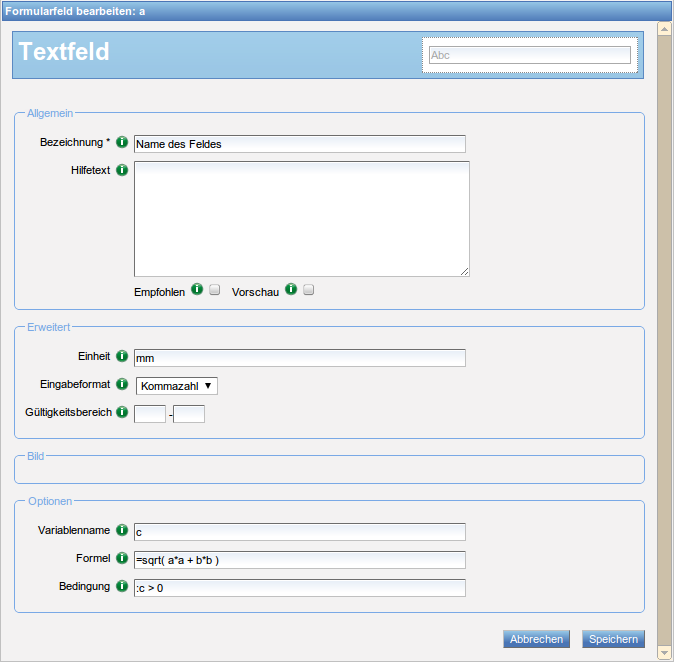
\includegraphics[scale=0.5]{figures/screenshot_spics_eingabe_neu}
\end{center}
\caption{Eingabe der DSL im Formulareditor}
\label{abb_screenshot_spics_eingabe}
\end{figure}

Hier wirft sich die Frage auf, ob es sinnvoll ist, die Angabe eines Constraints zu einem Feld, das durch eine Formel berechnet wird, zuzulassen. Meistens ist der Wert eines durch eine Formel berechneten Feldes ohnehin von anderen Feldern abhängig. Es erscheint also sinnvoll, die Validierung durch Constraints dort durchzuführen, um der Formel gültige Werte zu liefern. Andererseits muss eine Formel nicht von anderen Feldern abhängig sein\footnote{{Es kann durch Funktionen beispielsweise eine Formel erstellt werden, die einen Datumswert aus dem aktuellen Datum berechnet. Hier könnte ein Constraint der, z.B. vom Datum eines anderen Feldes abhängt, durchaus Sinn machen.}}. In der ersten Implementierung, die im Zuge dieser Arbeit durchgeführt wird, soll die Möglichkeit, ein Feld mit einer Formel und einem Constraint geichzeitig zu belegen, bestehen bleiben. Es bleibt zu evaluieren, inwieweit so eine Einschränkung, auch in Hinsicht auf eine Vereinfachung des User Interfaces und der damit eingehenden Verbesserung der Usability, sinvoll ist.

Beim Speichern wird ein Validator aufgerufen, der jedes der drei Felder gesondert validiert. Im Validator findet die Zyklenüberprüfung und die Überprüfung von Abhängigkeiten statt. Beim Speichern eines Formularelements sind mehrere Aspekte betreffend der DSL zu beachten:

\paragraph{Variablenname}
\begin{itemize}
	\item Der Variablenname darf nur einmal in dem Formular vorkommen.
	\item Der Variablenname darf nur aus Buchstaben und Ziffern bestehen, wobei das erste Zeichen ein Buchstabe sein muss.
	\item Um die Formeln nicht unübersichtlich werden zu lassen, wird die Länge der Variablen auf 15 Zeichen begrenzt.
\end{itemize}

\paragraph{Formel}
\begin{itemize}
	\item Alle Variablen, die in einer Formel verwendet werden, müssen bereits angelegt worden sein. Ein Anlegen der Variablen im Nachhinein soll nicht erlaubt werden, um die Konsistenz zu gewährleisten.
	\item Die Formeln eines Formulars dürfen keine zyklischen Abhängigkeiten enthalten (siehe Abschnitt \ref{implementierung_zyklenueberpruefung}).
	\item Die Formel darf sich nicht selbst referenzieren (also ein Verweis auf den Variablennamen des eigenen Feldes), da dies wiederum einer zyklischen Abhängigkeit entsprechen würde.
	\item Der Rückgabetyp der Formel muss dem Datentyp des Formelements entsprechen, da das Ergebnis der Formel sonst nicht zugewiesen werden kann.
\end{itemize}

\paragraph{Constraint}
\begin{itemize}
	\item Ein Constraint muss als Rückgabetyp Boolean haben, da er über die Gültigkeit der Eingaben entscheidet.
	\item Im Gegensatz zur Formel, darf sich ein Constraint auf den Wert des eigenen Feldes, sprich den eigenen Variablennamen beziehen. Dies ist not\-wen\-dig, um das eigene Feld zu validieren.
	
\end{itemize}

\section{Zyklenüberprüfung}
\label{implementierung_zyklenueberpruefung}

Ein essentieller Bestandteil der Validierung ist die Überprüfung auf zyklische Abhängigkeiten innerhalb eines Formulars. Diese Abhängigkeiten können als gerichteter Graph interpretiert werden: Enthält ein Formelement eine Formel mit Variablen, so sind alle Formelemente, die durch diese Variablen repräsentiert werden Nachfolger des Formularelements. Ist umgekehrt ein Formelement durch einen Variablennamen markiert, sind alle Formelemente, die eine Formel mit diesem Variablennamen enthalten, Vorgänger des Formelements. Abbildung \ref{abb_cycle_bmi_tree} zeigt den Graphen für das Beispielformular zur BMI-Berechnung.

\begin{figure}[ht]
\begin{center}
 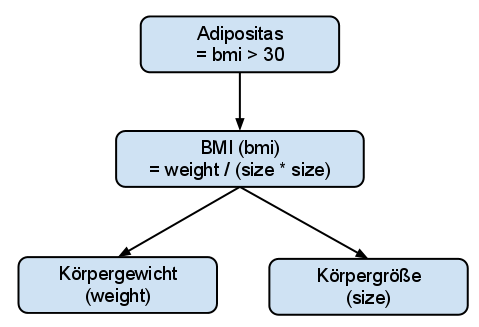
\includegraphics[scale=0.5]{figures/cycle_bmi_tree}
\end{center}
\caption{Baum der Abhängigkeiten im BMI-Formular}
\label{abb_cycle_bmi_tree}
\end{figure}

Die Interpretation der Abhängigkeiten als gerichteter Graph hilft bei der Überprüfung auf Zyklen. Ein Zyklus (oder Kreis) ist ein Weg von einem Knoten zu sich selbst \cite{Schl08}. Es gibt zwei grund\-sätz\-liche Algorithmen, die sich für die Überprüfung eignen: die Überprüfung durch Tiefensuche oder Breit\-en\-su\-che.

Die Tiefensuche ist ein Algorithmus, bei dem der Graph rekursiv abgearbeitet wird. Die bereits besuchten Knoten werden in einer globalen Liste abge\-spei\-chert. Wird ein Knoten besucht, der sich bereits in der Liste befindet, so liegt ein Zyklus vor. Durch Erweiterungen (Merken der Wege) können so alle Zyklen eines Graphen identifiziert werden.

Ein weniger mächtiger Algorithmus ist die Breitensuche. Diese ist ausreichend, wenn nur festgestellt werden soll, ob sich ein Knoten in einem Zyklus befindet oder nicht. Im Folgenden wird der Algorithmus zur Zyklenüberprüfung in der Implementierung (mittels Breitensuche) erläutert.

Die Eingabe ist das aktuelle Feld, das überprüft werden soll. Wenn keine Zyklen vorliegen, terminiert der Algorithmus. Wenn ein Zyklus gefunden wird, wird eine Exception geworfen. Ein Feld ist von einem anderen abhängig, wenn der Variablenname des Feldes in der Formel des anderen Feldes vorkommt.

\begin{enumerate}
  \item Überprüfe das aktuelle Feld, ob ein Variablenname und eine Formel vorhanden ist. Ist dies nicht der Fall, kann es nicht Teil eines Zyklus sein und die Überprüfung wird ohne Fehler beendet.
  
  \item Initialisiere die Menge \texttt{visited}. Sie enthält jene Felder, die bereits besucht wurden. 

  \item Füge den Variablennamen des aktuellen Feldes hinzu.

  \item Initialisiere die Menge \texttt{next}. Sie enthält jene Felder, die von den aktuell überprüften Feldern abhängen.

  \item Füge alle Variablen der Formel des aktuellen Feldes hinzu.

  \item Solange \texttt{next} nicht leer ist:

    \begin{enumerate}
      \item Wenn \texttt{visited} $\cup$ \texttt{next} $\neq$ \{\} : Es liegt ein Zyklus vor. Wirf Exception.
      \item Füge alle Elemente aus \texttt{next} zu \texttt{visited} hinzu.
      \item \texttt{next} = alle Nachfolger der Felder aus \texttt{next}.
    \end{enumerate}
\end{enumerate}


\section{Dateneingabe}
\label{implementierung_daten_eingabe}

Die Eingabe der medizinischen Daten in die Dokumentationssoftware ist der eigentliche Einsatzort der DSL. Hier werden die Formeln anhand der eingegebenen Daten berechnet und die Constraints überprüft. Vor der Implementierung werden allerdings einige Überlegungen benötigt, wie die Berechnung und Validierung der Werte durch die Aus\-führ\-ung der Formeln und Constraints am Besten umgesetzt wird.


\subsection{Aus\-führ\-ungszeitpunkt}

Ein Aspekt der Dateneingabe ist die Frage, wann die Formeln des Formulars ausgeführt werden. Im Beispiel des BMI-Rechners muss der BMI aus den Werten der Felder Kör\-per\-grö\-ße und Körpergewicht ausgerechnet werden. Es gibt mehrere Optionen, wann die Berechnung ausgelöst werden soll.

\begin{itemize}
	\item Beim Abspeichern eines Formulars: Die Felder, die durch Formeln berechnet werden, bleiben leer. Erst beim Speichern eines Formulars werden die abhängigen Felder berechnet. Wenn ein Fehler auftritt, wird der Benutzer zum Formular zurückgeleitet und aufgefordert, die Fehler zu beheben. Dies ist die ``sicherste'' Lösung, weil die asynchrone Kommunikation mit dem Server wegfällt. Diese Lösung ist allerdings nicht akzeptabel, da die Felder schon während des Ausfüllens berechnet werden sollen.

	\item In `Echtzeit' bei der Dateneingabe: Die Formeln werden nach der Eingabe eines Werts in ein Formularelement über einen Ajax-Validator berechnet. Der Eingabewert des Feldes wird nach der Eingabe\footnote{In der Implementierung wird, abhängig vom Typ des Eingabefeldes, entweder das \texttt{onblur}- oder \texttt{onchange}-Event des Formelements verwendet.} an den Server gesendet. Dort werden jene Felder, die vom eingegebenen Wert abhängen, berechnet und an den Client zurückgegeben, der die berechneten Werte in die ent\-sprech\-enden Felder einfügt.

	Die Möglichkeit der zusätzlichen wiederholten Berechnung nach dem Speichern bleibt allerdings bestehen.

	\item Auf Knopfdruck/Wunsch des Users: Die Werte der Felder werden nicht automatisch nach der Eingabe, sondern nur auf expliziten Wunsch des Users an den Server gesendet und dort berechnet. Zu\-sätz\-lich werden die Felder beim Speichern berechnet. Diese Lösung hätte den Vorteil, dass der Benutzer mehr Kontrolle über das Formular hat. Zu\-sätz\-lich werden etwaige Verzögerungen, die bei der `Echtzeit'-Lösung aufteten könnten vermieden.
\end{itemize}

In der Implementierung wurde der zweite Weg gewählt. Die Daten werden in Echtzeit an den Server gesendet und dort ausgewertet. Zu\-sätz\-lich werden die Felder noch einmal beim Speichern berechnet.

Die Frage der Auswertung stellt sich auch bei jenen Feldern, die mit Constraints belegt sind. Entweder werden die Constraints bereits beim Ausfüllen, oder erst beim Abspeichern evaluiert. Auch hier wurde eine Lösung aus beiden Möglichkeiten implementiert. 


\subsection{Aus\-führ\-ungsort}
\label{integration_ausfuehrungsort}

Webanwendungen bieten heutzutage dank Java\-Script die Möglichkeit, Berechnungen entweder clientseitig durchzuführen, oder das Ergebnis einer Berechnung mittels Ajax-Calls vom Server abzufragen und dann clientseitig weiter zu verarbeiten. Die Frage der client- oder serverseitigen Evaluierung der FXL stellt sich auch bei der Integration in SPICS.

\subsubsection{Clientseitige Evaluierung}

\begin{figure}[th]
\begin{center}
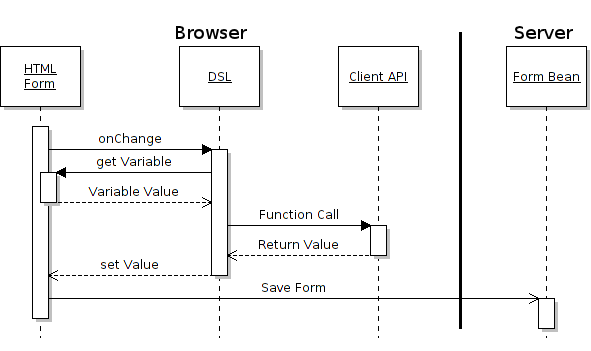
\includegraphics[scale=0.55]{figures/uml_seq_client_neu}
\end{center}

\caption{Clientseitige Lösung}
\label{abb_uml_seq_client}
\end{figure}


Grundsätzlich wäre eine clientseitige Evaluierung der Formeln möglich, indem man die DSL-Statements in Java\-Script übersetzt und im Browser ausführt. Die Übersetzung von FXL in Java\-Script ist möglich, da Java\-Script alle Sprachkonzepte, die FXL verwendet unterstützt\footnote{Tatsächlich das gleiche Verhalten wie Java\-Script zu erzeugen, ist nicht ganz so einfach, da Java\-Script bei manchen Operatoren ein anderes Verhalten an den Tag legt.}. Wenn eine Formel den Wert eines Feldes verändert, so wird dieser neue Wert im ent\-sprech\-enden Formularfeld gesetzt. Erst beim Speichern eines Formulars werden die berechneten und eingegebenen Werte an den Server gesendet, wo diese validiert und persistiert werden (Abbildung \ref{abb_uml_seq_client}).

Ein Schwachpunkt dieser Lösung ist, dass die in Java programmierten Funktionen, die in FXL verwendet werden können, nicht so einfach in Java\-Script übersetzt werden können wie die DSL-Statements selbst. Es ist also eine eigens für den Browser entwickelte API not\-wen\-dig, die alle Funktionen enthält, die der DSL auch am Server zur Verfügung stehen. Die Variablen können einfach aus den betreffenden Formularfeldern ausgelesen werden.

Eine Möglichkeit, den Overhead einer zusätzlichen clientseitigen Implementierung der Funktionen zu beseitigen, wäre die Weiterleitung der Funktionsaufrufe an den Server per Ajax-Call (Abbildung \ref{abb_uml_seq_client_hybrid}). Ein Bean am Applicationserver ruft die Methode in der Java-Implementierung auf und sendet den Rückgabewert zurück an den Browser. Der Nachteil ist, dass der Performance-Vorteil der clientseitigen Implementierung bei mehreren Funktionsaufrufen verloren geht.

\begin{figure}[h]
\begin{center}
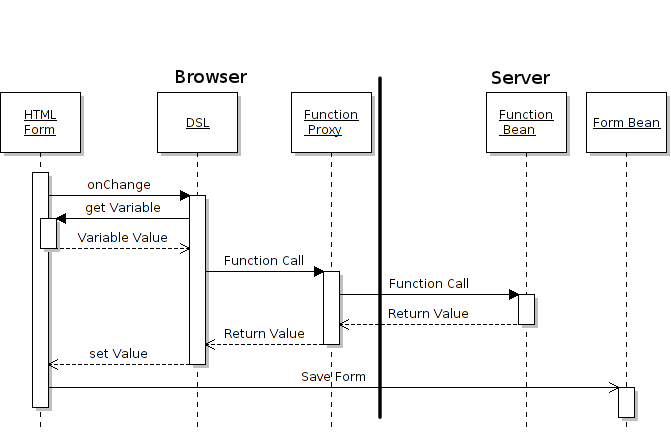
\includegraphics[scale=0.55]{figures/uml_seq_client_hybrid_neu}
\end{center}

\caption{Client- und serverseitige Hybridlösung}
\label{abb_uml_seq_client_hybrid}
\end{figure}

Ein weiterer Schwachpunkt der clientseitigen Lösung ist die Manipulierbarkeit von Skripten im Browser. Durch ent\-sprech\-ende Tools wie Firebug\footnote{http://getfirebug.com/}, können Nutzer das DOM und die Skripte manipulieren, und so eine korrekte Aus\-führ\-ung der DSL verhindern. Ein weiteres Defizit ist, dass die präzisen Fehlermeldungen, die für FXL definiert wurden, nun nicht nutzbar sind, da diese nicht in Java\-Script transferiert werden können.

\subsubsection{Serverseitige Evaluierung}

Die Alternative zur Evaluierung der Statements im Browser ist die Aus\-führ\-ung am Server (Abbildung \ref{abb_uml_seq_server}).

\begin{figure}[ht]
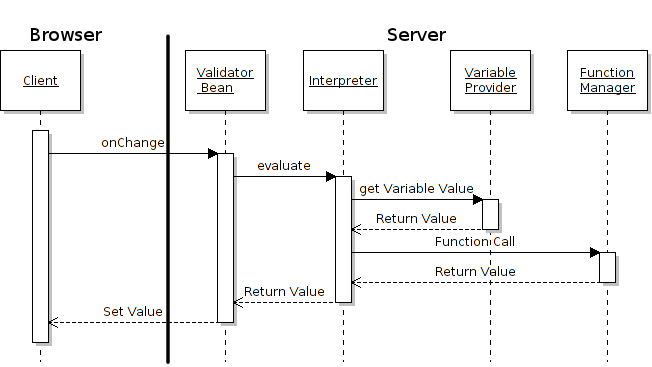
\includegraphics[scale=0.55]{figures/uml_seq_server_neu}
\caption{Aus\-führ\-ung am Server}
\label{abb_uml_seq_server}
\end{figure}

Das \texttt{onblur}- bzw. \texttt{onchange}-Event des Formularelements löst per JSF Ajax\-Support die Validierung des Formularelements am Applicationserver aus. Der eigens für die DSL implementierte DslValidator ruft die Komponente DslExecuter auf, die die DSL-Statements in korrekter hierarchischer Reihenfolge der Abhängigkeiten ausführt (vgl. Algorithmus in Abschnitt \ref{implementierung_integration_reihenfolge}). Für jede FXL-Formel wird ein Interpreter erstellt, der die Formel evaluiert und dabei auf die Implementierung des \texttt{VariableProvider} Interfaces und den Functionmanager zugreift. Zu\-sätz\-lich zu dem Feld, das das Event ausgelöst hat, werden auch die abhängigen Formularelemente neu gerendert.

Tritt bei der Aus\-führ\-ung der DSL-Statements ein Fehler auf, so wird eine ent\-sprech\-ende \texttt{FXLException} geworfen und über die Komponenten bis zum DslValidator weitergeleitet, wo diese abgefangen wird. Mithilfe des Fehlercodes wird eine FacesMessage erstellt und an den Context der Applikation übergeben. Diese Fehlermeldung wird im Browser beim betreffenden Formelement angezeigt.

Die serverseitige Lösung ist die einfachere Lösung, da die Aus\-führ\-ung einfach mittels FXL vorgenommen werden kann. Auch das Fehlerhandling erfolgt über die dafür vorgesehenen Exceptions, die dem Benutzer detailliertes Feedback geben. Bei der Integration im Zuge der praktischen Arbeit hat sich herausgestellt, dass die Antwortzeiten bei dieser Methode sehr gering sind. Ob die Verzögerung durch den Ajax-Call bei sehr komplexen Formularen eine unangenehme Verzögerung für den Benutzer darstellt, kann in einer weiteren Arbeit evaluiert werden. 


\subsection{Aus\-führ\-ungsreihenfolge}
\label{implementierung_integration_reihenfolge}

Die Aus\-führ\-ungsreihenfolge ist essentiell für die korrekte Auswertung der Formeln eines Formulars. Bevor ein Feld zur Berechnung herangezogen wird, muss sichergestellt werden, dass dieses selbst bereits berechnet wurde, wenn es eine Formel enthält. Wie bereits in Abschnitt \ref{implementierung_zyklenueberpruefung} erläutert, können die Abhängigkeiten in einem Formular als gerichteter zyklenfreier Graph gesehen werden. Wird ein Formularelement in der Formel eines anderen Elements verwendet, so kann dies als eine gerichtete Kante gedeutet werden.

Der folgende Algorithmus geht davon aus, dass keine Zyklen vorliegen. Die Zyklenfreiheit muss bereits beim Erstellen des Formulars sichergestellt werden (Abschnitt \ref{implementierung_zyklenueberpruefung}).

\begin{enumerate}
	\item Suche alle Felder, die einen Variablennamen, aber keine Formel beinhalten. Schreibe alle Werte der Felder in die Map \texttt{calculated<String, 			Result>}, wobei der Key der Variablenname ist und der Value der Wert des Feldes in einem \texttt{Result} Objekt.
	\item Erstelle eine Liste \texttt{formulas} aller Felder, die Formeln besitzen, sprich berechnet werden müssen.
	\item Solange \texttt{formulas} nicht leer ist, für jede Formel:
	
	\begin{enumerate}
		\item Hole alle Variablen aus der Tokenfolge der Formel.
		\item Wenn alle Variablen im KeySet von \texttt{calculated} sind:
		\begin{enumerate}
			\item Berechne die Formel.
			\item Wenn das Formelement der Formel einen Variablennamen hat, schreibe diesen mit dem berechneten Wert in \texttt{calculated}.
			\item Lösche die Formel aus \texttt{formulas}.
		\end{enumerate}	
		\item Wenn nicht alle Variablen bereits berechnet sind, ignoriere die Formel.
	\end{enumerate}	
	
\end{enumerate}

Der Algorithmus ist recht einfach: Zuerst werden alle Felder als berechnet angesehen, die selbst keine Formel beinhalten. Danach werden jene Felder berechnet, deren Formeln nur Variablen beinhalten, die auf bereits berechnete Felder verweisen. Durch die zugesicherte Zyklenfreiheit kann dieser Vorgang wiederholt werden, bis alle Felder berechnet sind.

Im Beispiel des BMI-Rechners (Abbildung \ref{abb_cycle_bmi_tree}) werden zuerst die Felder \emph{Körpergröße} und \emph{Körpergewicht} als berechnet markiert, da diese nicht von anderen Feldern abhängig sind. Danach werden die Felder mit Formeln, hier \emph{Adipositas} bzw. \emph{BMI}, in eine Liste ge\-spei\-chert, die in einer Schleife abgearbeitet wird. Wird zuerst versucht, das \emph{Adipositas}-Feld zu berechnen, wird festgestellt, dass das Feld \emph{BMI} noch nicht berechnet wurde und der Versuch verworfen. Danach wird das Feld \emph{BMI} aus den Feldern \emph{Körpergröße} und \emph{Körpergewicht} berechnet und aus der Liste entfernt. Beim nächsten Schleifendurchlauf kann nun die Formel der \emph{Adipositas}-Checkbox ausgewertet und aus der Liste gelöscht werden.

Bei der Aus\-führ\-ung wirft sich die Frage auf, wie vorgegangen werden soll, wenn ein Eingabefeld mit Variablenname noch nicht ausgefüllt wurde. In diesem Fall liefert die \texttt{lookup()}-Methode des \texttt{VariableProvider} ein \texttt{Result}-Objekt vom richtigen Datentyp, aber mit Wert \texttt{null} zurück. Die ganze Formel wird, wie im Abschnitt \ref{design_interpreter} beschrieben, zu einem \texttt{Result}-Objekt mit Wert \texttt{null} ausgewertet. Ist ein Feld also noch leer, werden auch die abhängigen Felder nicht mit einem Wert belegt. Wichtig ist jedoch, dass die Aus\-führ\-ung nicht unterbrochen wird und alle Felder, die nicht von einem nicht ausgewerteten Feld abhängen können, berechnet werden.



\section{Fehlerbehandlung}
\label{integration_fehlerbehandlung}

Durch die sehr detaillierten Fehlermeldungen der DSL-Implementierung ist es möglich, dem Benutzer ein genaues Feedback zu geben, wenn Probleme auftreten. Zu\-sätz\-lich zu den vorgegebenen Fehlern ist es sinnvoll, auch implementierungsspezifische Fehlermeldungen zu definieren.

Wenn Exceptions bei der statischen Analyse oder der Aus\-führ\-ung eines Statements auftreten, so müssen diese intelligent weitergeleitet und an der richtigen Stelle im System abgefangen werden, um einen reibungslosen Ablauf des Workflows zu ermöglichen, aber vor allem um den ordnungsgemäßen Betrieb des Systems nicht zu gefährden.

\subsection{Implementierungsfehler}

In der Dokumentationssoftware können Fehler an zwei Stellen auftreten: Bei der Modellierung eines Formulars und bei der Aus\-führ\-ung der Formeln und Constraints beim Ausfüllen eines Formulars. Jene Fehler, die beim Ausfüllen auftreten, wie etwa eine Division durch null, werden bereits von den in Abschnitt \ref{section_design_fehlerbehandlung} definierten Implementierungsfehlern abgedeckt. Wenn eine ent\-sprech\-ende \texttt{FXLException} geworfen wird, wird diese am Server abgefangen. Anhand des Fehlercodes wird die ent\-sprech\-ende internationalisierte Nachricht erstellt (siehe unten). 


\begin{table}
\begin{tabular}[ht]{|c | p{11cm}|}
	\hline
	\textbf{Code} & \textbf{Beschreibung}\\
	\hline
  	\hline
  	4xx  & \multicolumn{1}{|l|}{\textsc{Implementierungsfehler}} \\
  	\hline
  	400  & Allgemeiner/unbekannter Implementierungsfehler    \\
  	\hline
  	411  & Ungültiger Variablenname    \\
  	\hline
  	412  & Variablenname zu lang    \\
  	\hline
  	413  & Variablenname bereits vorhanden   \\
  	\hline
  	414  & Die Formel erzeugt zyklische Abhängigkeiten    \\
  	\hline
  	415  & Die Formel enthält unbekannte Variablen    \\
  	\hline
  	416  & Rückgabetyp der Formel stimmt nicht mit Datentyp des Formelements überein    \\
  	\hline
  	417  & Rückgabetype eines Constraints ist nicht Boolean    \\
  	\hline
\end{tabular}
\caption{Fehlercodes für Implementierungsfehler}
\end{table}

Neu und spezifisch für den Einsatzbereich der DSL sind jene Fehler, die beim Erstellen der Formulare auftreten. Diese decken vor allem Fehler des Formats von Variablen, der logischen Struktur der Abhängigkeiten und der Rückgabetypen ab.



\subsection{Internationalisierung}

Die Internationalisierung der Fehlermeldungen erfolgt mit ``Boardmitteln'' von Seam\footnote{ vgl. http://docs.jboss.org/seam/latest/reference/en-US/html/i18n.html, 21.12.2011}. Die Labels werden in Properties-Files für alle unterstützten Sprachen ge\-spei\-chert (Listing \ref{listing_error_de} bzw. \ref{listing_error_en}).

\begin{lstlisting}[float = htbp,caption={Deutsche Fehlermeldungen },label=listing_error_de]
error.dsl.202=Ungueltige Kombination von Typen fuer Operator {0}: {1}, {2}
error.dsl.211=Variable nicht gefunden: {0}
error.dsl.212=Variable mehrfach definiert: {0}
\end{lstlisting}

\begin{lstlisting}[float = htbp,caption={Englische Fehlermeldungen},label=listing_error_en]
error.dsl.202=Invalid type combination for operator {0}: {1}, {2}
error.dsl.211=Variable not found: {0}
error.dsl.212=Variable defined more than once: {0}
\end{lstlisting}

Zur Identifizierung der Labels wird der Fehlercode der Exception verwendet. Um das Feedback duch fehlerspezifische Informationen anzureichern, werden die Argumente der Fehlermeldungen, wie in Listing \ref{listing_error_de} bzw. \ref{listing_error_en} ersichtlich verwendet.






\part{Ergebnis}
\label{part_ergebnis}

\chapter{Ergebnis}
\label{chapter_ergebnis}

Im Zuge der vorliegenden Arbeit wurde eine Domain Specific Language (DSL) entwickelt und in ein existierendes Studiensystem integriert.

Die entwickelte DSL, die Form Expression Language (FXL), wurde als eigenständige Java-Bibliothek entworfen. Als solche ist diese unabhängig vom konkreten Einsatzsystem. Über die entwickelten Schnittstellen ist die Bibliothek somit in beliebige Java-Anwenundgen integrierbar.

Beim Entwurf der FXL wurde auf eine einfache Syntax, die sich an bekannten Anwendungen wie Tabellenkalkulationssoftware oder Taschenrechner orientiert, Wert gelegt. Die Sprache definiert einzelne Statements, die durch logische Operatoren, arithmetische Operatoren und Vergleichsoperatoren, sowie Klammerungen, definiert werden. Ferner enthält die Syntax auch Variablen, die als Referenzen auf Werte  in die Statements eingebunden werden können. Über eine Schnittstelle kann eine externe Implementierung einer Symboltabelle eingebunden werden, die Variablennamen in konkrete Werte auflöst. Zusätzlich können in Java entwickelte, wohldefinierte Funktionen in die Sprache integriert werden. Die FXL unterstützt vier Datentypen: Ganzzahlen, Gleitkommazahlen, Datumswerte und boolesche Werte.

Um dem Benutzer Feedback über die eingegebenen Statements geben zu können, existiert eine detaillierte Fehlerbehandlung über eine Hierarchie von eigens definierten Exceptions. Diese Exceptions bilden Fehler in den Phasen syntaktische Analyse, semantische Analyse, sowie Laufzeit ab. Jede dieser Fehlerkategorien definiert wiederum detaillierte Fehlercodes und Parameter, um die Ursache eines Fehlers einfach nachvollziehbar darzustellen.

Bei der Entwicklung der FXL wurde auf einen testgetriebenen Entwicklungsablauf achtgegeben. Für jedes neue Feature (diverse Operatoren, Variablen, Funktionen, Fehler etc.) wurden vor der Implementierung Testfälle definiert, die das korrekte Verhalten der Sprache abbilden. Dadurch konnte eine effiziente Entwicklung und ein testbares Design erreicht werden.

Bei der Integration der FXL in eine bestehende Anwendung sind unterschiedliche Aspekte zu beachten. Als Integrationsbeispiel wird die Einbettung der DSL in die medizinische Studiensoftware SPICS vorgenommen.

Zuerst muss der Workflow des Zielsystems analysiert werden. Dies ist notwendig, um die Anknüpfungspunkte für die Eingabe der Ausdrücke sowie die Ausführung des Interpreters zu ermitteln. Der nächste Schritt sind die Änderungen im Datenmodell, um die Statements im System zu persistieren.

Bei der Integration in eine Webanwendung wie SPICS, sind Gedanken über den Ort und die Zeit der Ausführung unerlässlich. Durch die Trennung in Client und Server, bieten sich mehrere Möglichkeiten mit unterschiedlichen Stärken und Schwächen. Für die Integration in diese Arbeit wurde eine serverseitige Lösung gewählt. Die Statements werden allerdings in Echtzeit, bereits bei der Eingabe der Daten, per Ajax-Calls an den Server übertragen und dort ausgewertet.

Da Variablen in den FXL-Statements im Studiensystem auf andere Formularfelder im selben Formular zeigen, muss gewährleistet werden, dass sich diese in abhängigen Formularfeldern nicht gegenseitig referenzieren. Dazu wird ein Baum von Abhängigkeiten der Formularfelder gebildet, der auf Zyklenfreiheit untersucht wird. Dieser Baum gibt auch die Ausführungsreihenfolge der Statements vor. Vor der Auswertung eines Statements, müssen zuerst die von diesem referenzierten Felder ausgewertet werden.

Zuletzt müssen auch die Fehler, die bei Eingabe der Statements bzw. bei deren Ausführung auftreten können, behandelt werden. Da die semantische Analyse und die Ausführung am Server vorgenommen wird, können die in der FXL definierten Fehler abgefangen, und an den Client zurückgegeben werden. Dabei erfolgt über die Fehlercodes eine Umwandlung der Fehler in applikationsabhängige, internationalisierte Fehlermeldungen.



\chapter{Ausblick}
\label{chapter_ausblick}

Im Verlauf der Arbeit haben sich einige Gedanken herauskristallisiert, die sich für weitere Arbeiten, über den Umfang dieser Diplomarbeit hinaus, anbieten. Diese  Themen werden im Folgenden kurz beschrieben. 

In der Implementierung wurde die Integration der Form Expression Language in SPICS nur für drei verschiedene Formelemente vorgenommen, die ausreichen, um die vier unterstützten Datentypen zu repräsentieren: Textfelder für die numerischen Typen, sowie Checkboxen für boolesche Werte und Datepicker für Datumswerte. Für die Verwendung von weiteren Formelementen wie Listen, Drop-Downs und Radiobuttons können Überlegungen angestellt werden, wie Werte dieser Elemente mit der FXL verarbeitet werden können.

Referenzierungen in den Formeln der FXL lassen sich momentan nur auf Formularfelder innerhalb eines Formulars vornehmen. Da für einen Patienten in SPICS unterschiedliche Formulare angelegt werden können, kann die Referenzierung von Feldern aus anderen Formularen eine weitere Anforderung darstellen. Dafür kann die Implementierung der Variable Provider dahingehend geändert werden, dass ein Lookup von Variablen auch Werte bereits persistierter Formulare berücksichtigt. 

Eine weitere Form von Abhängigkeiten zwischen Formularfeldern könnten eingabeabhängige Berechnungen darstellen. Damit sind Abhängigkeiten zwischen Feldern gemeint, die Werte je nach vorhandener Eingabe berechnen. Im Beispiel des Body Mass Index (BMI) Rechners, der aus Körpergröße und Körpergewicht den BMI berechnet, könnte eine solche eingabeabhängige Berechnungwie folgt aussehen. Aus zwei beliebigen Feldern wird der dritte Wert automatisch berechnet. Werden also zuerst das Gewicht und der BMI eingegeben, wird automatisch die Körpergröße ermittelt. Inwieweit das durch Umformen von Statements der FXL möglich ist, ist zu evaluieren.

Auch die Form Expression Language selbst lässt Raum für Erweiterungen in mancherlei Hinsicht. Für eine formularübergreifende Referenzierung könnte etwa die Syntax für Variablennamen modifiziert werden. Eine weitere mögliche Erweiterung stellt die Einführung eines Datentyps für Zeichenketten, mit entsprechen Auswirkungen auf die Syntax der Sprache sowie die Semantik der Operatoren, dar. Eine zusätzliche Möglichkeit stellt die Definition weiterer Operatoren dar. In der Implementierung dieser Arbeit kann der ganzzahlige Rest einer Division (Modulo) nur durch eine eigene Funktion berechnet werden. Für diese Berechnung könnte, wie in anderen Sprachen üblich, der Operater \texttt{\%} eingeführt werden. Auch eigene logische Operatoren für exklusives Oder und Implikation sind denkbar. Diese logischen Operatoren müssen momentan durch die vorhandenen Grundoperatoren ausgedrückt werden.

Ein weiteres Thema sind die nichtfunktionalen Eigenschaften der Integration im Studiensystem. Vor allem in Hinsicht Usability kann die Implementierung einer Evaluierung unterzogen werden. Die Akzeptanz beim Endanwender kann durch User-Tests bestätigt oder widerlegt werden. Auch die Eingabe der Statements lässt Raum für Verbesserungen im User Interface. Eine Möglichkeit wäre beispielsweise Syntax Highlighting oder Code Completion anzubieten, um die Eingabe angenehmer zu gestalten und Fehler zu vermeiden. Auch in Hinblick auf die Performance der Sprache, sowie die Integration in das Studiensystem, können Untersuchungen vorgenommen werden. Vor allem die Möglichkeiten einer teilweisen clientseitigen Berechnung, wie in Abschnitt \ref{integration_ausfuehrungsort} dargelegt, können Thema einer weiteren Untersuchung sein.

\chapter{Zusammenfassung}
\label{chapter_zusammenfassung}

Das Thema dieser Arbeit entstand aus der Anforderung, Formulare in einer Webanwendung semantisch dahingehend anzureichern, dass flexible Berechnungen und Validierungen formelementübergreifend vorgenommen werden können. Im Rahmen der Arbeit wurde eine einfache Ausdruckssprache entwickelt und in ein medizinisches Studiensystem integriert.

Der erste Teil der Arbeit beschäftigt sich mit den technischen und theoretischen Grundlagen, die zum Verständnis des Textes notwendig sind. Zunächst wurde der Begriff der Domain Specific Language (DSL) diskutiert, eine Einteilung vorgenommen und Beispiele für bekannte DSLs vorgestellt. Danach wurden die theoretischen Grundlagen erarbeitet und eine Übersicht über Werkzeuge zum Entwurf von Sprachen geboten. Den Abschluss des ersten Teils bildet eine Übersicht über wissenschaftliche Arbeiten im Bereich der Modellierung von Webformularen.

Im zweiten Teil wird der Entwicklungsprozess der Form Expression Language (FXL), der sich in die Phasen Entscheidung, Analyse, Entwurf, Implementierung und Test gliedert, beschrieben. Zuerst wurde eine Entscheidung für eine eigene externe DSL getroffen und begründet. Danach wurden die Anforderungen an die Sprache analysiert und das Design der Sprache in Hinsicht auf die notwendigen Features wie Datentypen, Operatoren, Funktionen und Fehlerbehandlung, sowie Syntax und Semantik entwickelt. Danach wurden die Implementierungsdetails der FXL dargelegt. Den Abschluss des Teils bildet eine Abhandlung über das Testen der erstellten Software.

Der dritte Teil behandelt die Integration der Sprache in ein existierendes medizinisches Studiensystem. Zuerst wurde das Studiensystem SPICS kurz vorgestellt und die Architektur sowie die verwendeten Technologien beschrieben. Danach wurden die verschiedenen Aspekte der Integration der Sprache in SPICS veranschaulicht.

Der vierte Teil gibt einen Ausblick auf weitere Themen und Möglichkeiten, die sich im Zuge der Arbeit aufgetan haben und bietet eine zusammenfassende Übersicht über die Themen der Arbeit.

Ein Schwerpunkt der Arbeit war die praktische Implementierung der FXL, sowie die Integration in das medizinische Studiensystem. Die Arbeitsschritte entsprechen im Grunde den in der Arbeit dargestellten Schritten, mit dem Unterschied, dass die praktische Umsetzung natürlich ein iterativer Prozess war. Zuerst wurden die Anforderungen und das Zielsystem analysiert und eine Übersicht über das wissenschaftliche Feld erstellt. Danach wurden diverse Tools und Möglichkeiten zur Umsetzung der Sprache in Hinsicht auf die Anforderungen evaluiert. Im nächsten Schritt erfolgte die testgetriebene Implementierung der FXL, in der die Anforderungen iterativ überarbeitet und immer detaillierter spezifiziert wurden. Eine besondere Herausforderung war die Integration in das vorhandene Studiensystem, da auf die Besonderheiten des Systems, wie die Technologien oder das Datenmodell, eingegangen werden musste. Das Ergebnis der praktischen Arbeit ist eine funktionierende Implementierung gemäß der Problemstellung der schriftlichen Arbeit.







%\chapter{Terms and abbreviations}
%


AST - Abstract Sysntax Tree, CST Concrete Syntax Tree, GPL - General Purpose Language , Syntax, Semantik, Statement

Constraint - Bedingung



\begin{flushleft}
\bibliographystyle{plain}
\bibliography{biblio}
\end{flushleft}


\listoftables
\listoffigures
\lstlistoflistings

\appendix
% include appendexes here
\chapter{Grammatik}

\begin{lstlisting}[caption={Grammatik der FXL},label=listing_fxl_grammar]
grammar FXL;

options {
  language = Java;
  output   = AST;
}

tokens {
  OR  = 'OR';
  AND = 'AND';
  NOT = 'NOT';
  GT  = '>'; //greater then
  GE  = '>='; //greater then or equal
  LT  = '<'; //lower then
  LE  = '<='; //lower then or equal
  EQ  = '=';
  NEQ = '!='; //Not equal
  PLUS = '+';
  MINUS = '-';
  MULTIPLY = '*';
  DIVISION = '/';
  CALL;
}

@header {
package at.ac.tuwien.fxl;
}

@members {
    public void displayRecognitionError(String[] tokenNames,
                                        RecognitionException e) {
        String hdr = getErrorHeader(e);
        String msg = getErrorMessage(e, tokenNames);
        throw new RuntimeException(+e.index+"");
    }
}


@lexer::header {
package at.ac.tuwien.fxl;
}

statement 
  :  ('='|':')! expression 
  ;

expression
	: booleanAndExpression ('OR'^ booleanAndExpression)*
	;

booleanAndExpression
  :
  booleanNotExpression ('AND'^ booleanNotExpression)*
  ;

booleanNotExpression
  :
  ('NOT'^)? booleanAtom
  ;

booleanAtom
  :
  | compareExpression
  ;

compareExpression
  	:
  	commonExpression (('<' | '>' | '=' | '<=' | '>=' | '!=' )^ commonExpression)?
  	;

commonExpression
  :
  multExpr (( '+'^ | '-'^ ) multExpr)*
  ;

multExpr
  :
  atom (('*'|'/')^ atom)*
  | '-'^ atom
  ;

atom
  :
  INTEGER
  | DECIMAL
  | BOOLEAN
  | DATE
  | ID
  | '(' expression ')' -> expression
  | functionCall
  ;

functionCall
  :
  ID '(' arguments ')' -> ^(CALL ID arguments?)
  ;
  
arguments
  :
  (expression) (','! expression)*
  |  WS
  ;

BOOLEAN
  :
  'true'
  | 'false'
  ;

ID
  :
  ('a'..'z' | 'A'..'Z')+ ('a'..'z' | 'A'..'Z' | '0'..'9')*
  ;

INTEGER
  :
  ('0'..'9')+ 
  ;

DECIMAL
  :
  ('0'..'9')+ ('.' ('0'..'9')*)
  ;

DATE
  :
  '!' '0'..'9' '0'..'9' '0'..'9' '0'..'9' '-' '0'..'9' '0'..'9' '-' '0'..'9' '0'..'9'( '-' '0'..'9' '0'..'9' ':''0'..'9' '0'..'9' (':''0'..'9' '0'..'9')?)?
  ;

WS
  :  (' '|'\t' | '\n' | '\r' | '\f')+ { $channel = HIDDEN; };

\end{lstlisting}




\end{document}


